\documentclass[a4paper, 10pt]{article}
\usepackage[english]{babel}
\usepackage[T1]{fontenc}
\usepackage[utf8]{inputenc}
\usepackage[left=1.5cm, right=2cm]{geometry}
\usepackage{fancyhdr}
\usepackage{graphicx}
\usepackage{lastpage}
\usepackage{ragged2e}
\usepackage[yyyymmdd]{datetime}
\usepackage[acronym,nonumberlist]{glossaries}
\usepackage{iftex}
\usepackage{afterpage}
\usepackage{lscape}
\usepackage[table]{xcolor}
\usepackage{tcolorbox}

\DeclareUnicodeCharacter{200B}{{\hskip 0pt}}

% Glossary

\makeglossaries
\newglossaryentry{node}
{
        name=node,
        description={TODO! A fundamental entity in the Golem p2p network.}
}

\newglossaryentry{comp}
{
        name=computational resources,
        description={TODO! Any resources which allow to run a program. 
					In practice a single traditional computer or a cluster of computers.}
}

\newglossaryentry{requestor}
{
        name=requestor,
        description={TODO! A node which needs computational power. It defines the payload descriptor 
					and sends out demand order to find requestors.}
}

\newglossaryentry{provider}
{
        name=provider,
        description={TODO! A node that has computation resources to offer. It creates and sends out the offers. 
					One provider might be managing many computers (e.g. in case of a datacenter)}
}

\newglossaryentry{payload}
{
        name=payload,
        description={TODO! The computer program code, Docker or VM image, as well as the
					configuration and/or input data, which the requestor intends to have deployed
					and executed by the provider node(s)}
}

\newglossaryentry{plane}
{
        name=plane,
        description={}
}

\newglossaryentry{layer}
{
        name=layer,
        description={}
}

\newglossaryentry{namespace}
{
        name=namespace,
        description={}
}

\newglossaryentry{aspDim}
{
        name=aspect dimension,
        description={}
}

\newglossaryentry{service}
{
        name=service,
        description={}
}

\newglossaryentry{resource}
{
        name=resource,
        description={}
}

\newglossaryentry{demand}
{
        name=demand,
        description={TODO! Demand is created by Requestors and contains description of the
					payload, including properties telling what capabilities the payload might
					require (e.g. specific hardware architecture or features) and optionally other
					conditions which ought to be satisfied by the provider nodes (e.g. asking only
					for nodes which are located within specific country). Most of the content of the
					Demand is opaque for the Golem network}
}

\newglossaryentry{offer}
{
        name=offer,
        description={TODO! Offer is created by Provider nodes and contains the description of the
					computing resources the node has to offer, as well as any optional conditions
					for their use (e.g. limiting their availability only to certain requestor
					nodes).}
}

\newglossaryentry{proposal}
{
        name=proposal,
        description={TODO! The object which includes all the Demand/Offer/Proposal properties. 
					This is a JSON object in "flat convention" - where keys are full property names and 
					their values indicate properties.}
}

\newglossaryentry{agreement}
{
        name=agreement,
        description={TODO! The object which includes all the Demand/Offer/Proposal properties. 
					This is a JSON object in "flat convention" - where keys are full property names and 
					their values indicate properties.}
}

\newglossaryentry{invoice}
{
        name=invoice,
        description={TODO! An Invoice is an artifact issued by the Provider to the Requestor, 
					in the context of a specific Agreement. It indicates the total Amount owed by 
					the Requestor in this Agreement. 
					No further Debit Notes shall be issued after the Invoice is issued. 
					The issue of Invoice signals the Termination of the Agreement. 
					No Activity execution is allowed after the Invoice is issued.}
}

\newglossaryentry{property}
{
        name=property,
        description={}
}

\newglossaryentry{debit}
{
        name=debit note,
        description={A Debit Note is an artifact issued by the Provider to the Requestor, in the context of a specific Activity. 
					It is a notification of Total Amount Due incurred by the Activity until the moment the Debit Note is issued. 
					This is expected to be used as trigger for payment in upfront-payment or pay-as-you-go scenarios.}
}

\newacronym{gn}{GN}{Golem Node}
\newacronym{ga}{GA}{Golem Agent}
\newacronym{gc}{GC}{Golem Client}
\newacronym{gad}{GAD}{Golem Agent Daemon}
\newacronym{gac}{GAC}{Golem Agent Console}
\newacronym{gm}{GM}{Golem Manager}
\newacronym{gsm}{GSM}{Golem Schedule Manager}
\newacronym{gpg}{GPG}{Golem Payment Gateway}
\newacronym{gtk}{GTK}{Golem Toolkit}
\newacronym{gms}{GMS}{Golem Market Service}
\newacronym{gas}{GAS}{Golem Activity Service}
\newacronym{gps}{GPS}{Golem Payment Service}
\newacronym{gns}{GNS}{Golem Net Service}
\newacronym{gsb}{GSB}{Golem Service Bus}
\newacronym{gmsapi}{GMS API}{Golem Market Service API}
\newacronym{gasapi}{GAS API}{Golem Activity Service API}
\newacronym{gpsapi}{GPS API}{Golem Payment Service API}
\newacronym{gar}{GAR}{Golem Abstraction Resource}
\newacronym{res}{RES}{Resource}
\newacronym{up}{UP}{User Plane}
\newacronym{epp}{EPP}{External Provider Plane}
\newacronym{gp}{GP}{Golem Plane}
\newacronym{gacp}{Gacp}{Golem agent console point}
\newacronym{grp}{GRp}{Golem REST point}
\newacronym{gmp}{Gmp}{Golem market point}
\newacronym{gap}{Gap}{Golem activity point}
\newacronym{gpp}{Gpp}{Golem payment point}
\newacronym{gnp}{Gnp}{Golem net point}
\newacronym{Grp}{Grp}{Golem resource point}
\newacronym{Gsp}{Gsp}{Golem service point}
\newacronym{gntw}{Gntw}{Golem network}
\newacronym{pl}{PL}{Platform Layer}
\newacronym{il}{IL}{Integration Layer}
\newacronym{bl}{BL}{Business Layer}


% ToC Env

\pagenumbering{arabic}
\setcounter{secnumdepth}{5}
\setcounter{tocdepth}{5}

\makeatletter
\newcommand\subsubsubsection{\@startsection{paragraph}{4}{\z@}{-2.5ex\@plus -1ex \@minus -.25ex}{1.25ex \@plus .25ex}{\normalfont\normalsize\bfseries}}
\newcommand\subsubsubsubsection{\@startsection{subparagraph}{5}{\z@}{-2.5ex\@plus -1ex \@minus -.25ex}{1.25ex \@plus .25ex}{\normalfont\normalsize\bfseries}}
\makeatother

\renewcommand{\dateseparator}{--}

% Header and Footer Definition

\pagestyle{fancy}
\renewcommand{\headrulewidth}{0.4pt}
\renewcommand{\footrulewidth}{0.4pt}
\fancyhf{}
\fancyhead[R]{\bfseries Golem Network Architecture Overview}
\fancyfoot[L]{
    \raggedright{Author: P. Rekucki, M. Rakowski \\ Company: Golem Factory}
    }
\fancyfoot[C]{
    \centering{Draft \\ Propertiary}
    }
\fancyfoot[R]{
    \raggedleft{Date: \today \\ Page: \thepage\ of \pageref{LastPage}}
    }

\begin{document}

% Title Page

\thispagestyle{empty}
\begin{flushright}
    
\includegraphics[width=100bp]{Golem.png}
\end{flushright}

\vskip4cm

\begin{flushleft}
    \huge Functional and System Architecture Document
\end{flushleft}
\hrule
\begin{flushleft}
    \LARGE Golem Network Architecture Overview
\end{flushleft}

\vskip8cm
\hrule

\begin{center}
    \Large Warsaw 2024
\end{center}

\break

% ToC

\tableofcontents

\newpage

% Sections Files

%\section{Scope}
\section{Scope}

%\section{Reference}
\section{Reference}

%\section{Definition of terms and Abbreviations}
\glsaddall

\section{Definition of terms and Abbreviations}

\subsection{Terms}

For the purposes of the present document, the following terms apply:

\printglossary[title={}]

%\subsection{Symbols}

\subsection{Abbreviations}

For the purposes of the present document, the following abbreviations apply:

\printglossary[type=\acronymtype,title={}]






%\section{Framework Concept}
\section{Framework Concept}

\subsection{Introduction}

The Golem System is a framework for trading computing power in the Peer2Peer (P2P) model.
Settlement of computing power usage takes place in the Etherium network and its derivatives.

The framework consists of a set of basic components and dependencies between them, 
as well as programming elements that allow for the creation of decentralized and distributed
applications and services using the Golem trading model.

These are:

\begin{itemize}

\item protocols
\item libraries
\item API
\item implementation of sample components

\end{itemize}

The goal of the Golem System is to provide

\begin{itemize}

\item portability
\item ease of installation
\item flexibility

\end{itemize}

In this chapter, the general concept of the Golem network architecture will be presented. 
Both the assumptions and elements of the network, applications, services, protocols will be 
described in the most abstract way possible, so as not to lose the idea of ​​solving the system 
due to the complexity of the processes taking place in it.

A detailed description of the components will be described later in the document.

%\subsection{Definitions}
%\begin{description}
%\item[Plane] This is a set of elements (physical, virtual or their abstractions),
%applications, services, protocols, functions that allow for internal
%and external communication, their configuration and monitoring at all layers.
%\end{description}

\newpage

\subsection{Abstract Architecture}

The architecture of the Golem System will be presented on three planes 

(Please see Figure ~\ref{fig:BDC} on page ~\pageref{fig:BDC}):

\begin{enumerate}
	\item Golem Plane (GP)
	\item User Plane (UP)
	\item External Provider Plane (EPP)
\end{enumerate}

\begin{figure}[H]
    \centering
    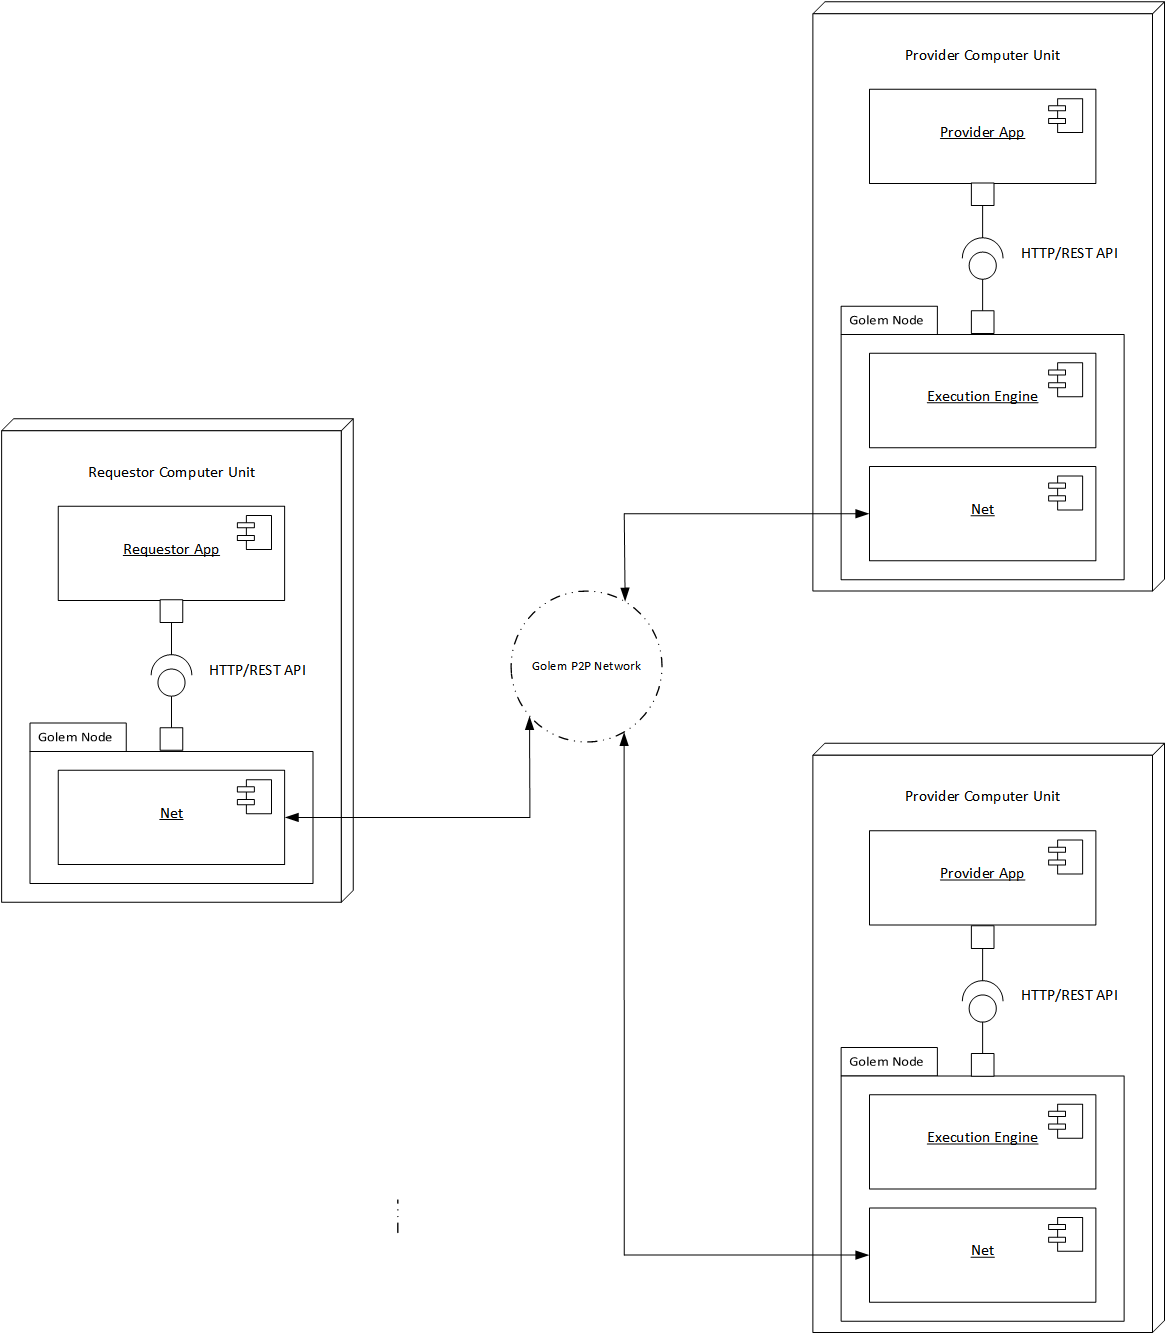
\includegraphics[width=12cm,angle=0]{./diag/Abstract/BasicDeployment-Abstract.png}
    \caption{Basic Deployment Concept}
	\label{fig:BDC}
\end{figure}

The Golem Plane is the basis on which nodes called Golem Nodes are defined, which build the Golem Network 

(Please see Figure ~\ref{fig:BPC} on page ~\pageref{fig:BPC}).

\begin{figure}[H]
    \centering
    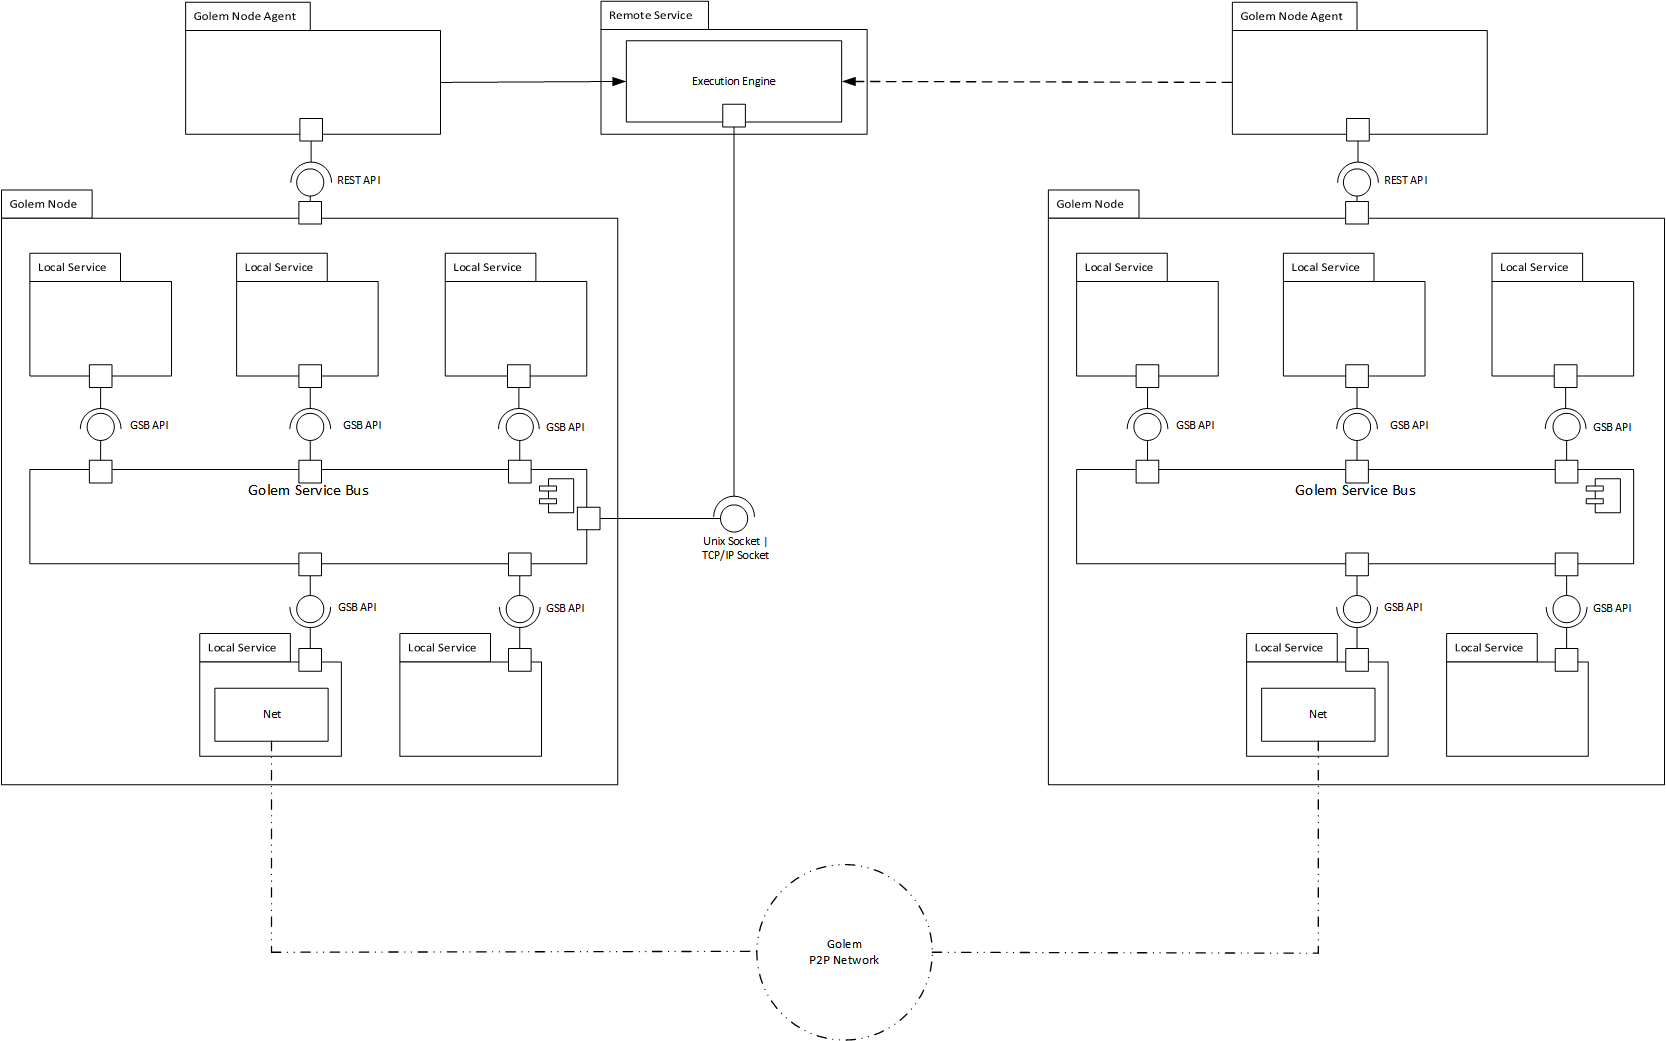
\includegraphics[width=18cm,angle=0]{./diag/Abstract/BasicPackages-Abstract.png}
	\caption{Basic Packages Concept}
    \label{fig:BPC}
\end{figure}

Each node consists of a set of core applications, core services
and core protocols enabling communication, configuration and monitoring 
on all layers of decentralized and distributed business processes.
Business processes are implemented on the User Plane using functions of 
core components of applications, services and protocols through their API.
The External Operator Plane is used for specific functions implemented
outside the Golem Network but used by this network. An example is the availability of
payments in cryptocurrencies.

The above Planes with their component elements distributed over three main layers 
are shown in the figure :

\begin{enumerate}
	\item Platform Layer (PL)
	\item Integration Layer (IL)
	\item Buisness Layer (BL)
\end{enumerate}

In the Platform Layer (PL) there is the Golem Agent (GA) element,
which allows you to create a Golem Node (GN) from a computer unit.
Golem Node is a member of the Golem Network (Gntw).

In the Integration Layer (IL) there is the Golem Agent console (GAC) and Golem Toolkit (GTK).
The Golem Agent console consists of tools for configuring and monitoring the created applications and services
and managing the Golem Agent element, which is a daemon of the created node (GN).
The Golem Toolkit is a set of tools, APIs that allow you to create decentralized and distributed applications and services
on the Golem network infrastructure and using the Golem commercial model.

In the Business Layer (BL) there is the user plane (UP) and the external provider plane (EPP).

In the user plane (UP), decentralized applications and services of the Golem network are implemented.
Users can use service and application templates created in the form of the "standards - change the name" framework specification.

This layer defines user roles that can be assigned to Golem nodes depending on the aspect of the node's computational resources and/or the service it provides.

The external provider layer (EPP) is used to handle payments that take place on the Etherium network and its derivatives.
This layer can be used to define and implement connections to other application and service networks.

%\afterpage{
%\begin{landscape}
%	\begin{figure}[htbp]
%		\centering
%		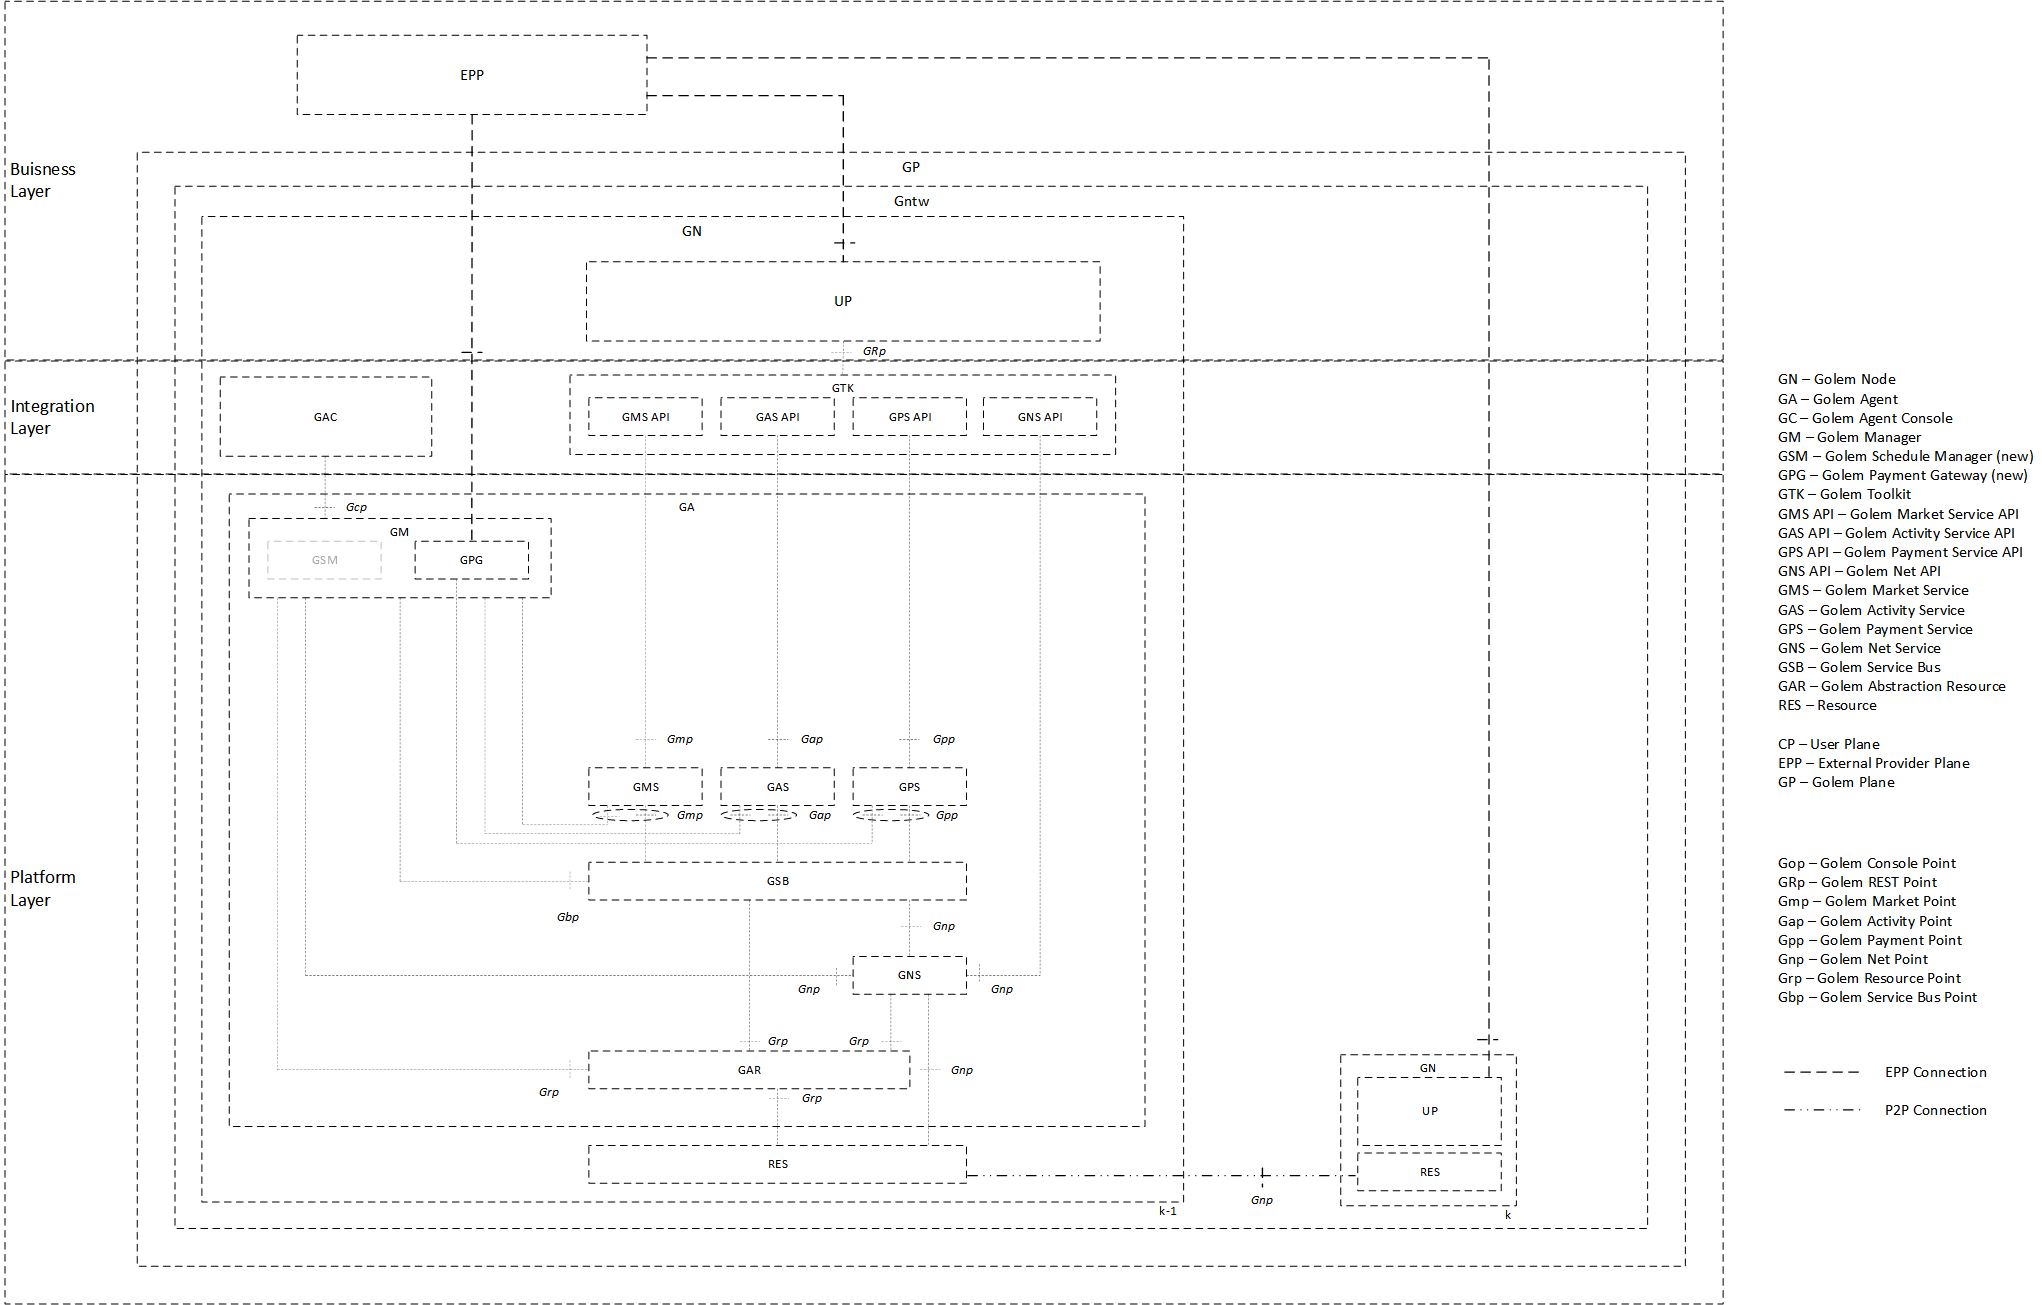
\includegraphics[width=\hsize]{./diag/Abstract/GolemSystemLayers-Abstract.png}
%		\caption{Abstraction Architecture Diagram}
%		\label{fig:Arch}
%	\end{figure}
%\end{landscape}
%}


(Please see Figure ~\ref{fig:DPC} on page ~\pageref{fig:DPC})

\begin{figure}[H]
    \centering
    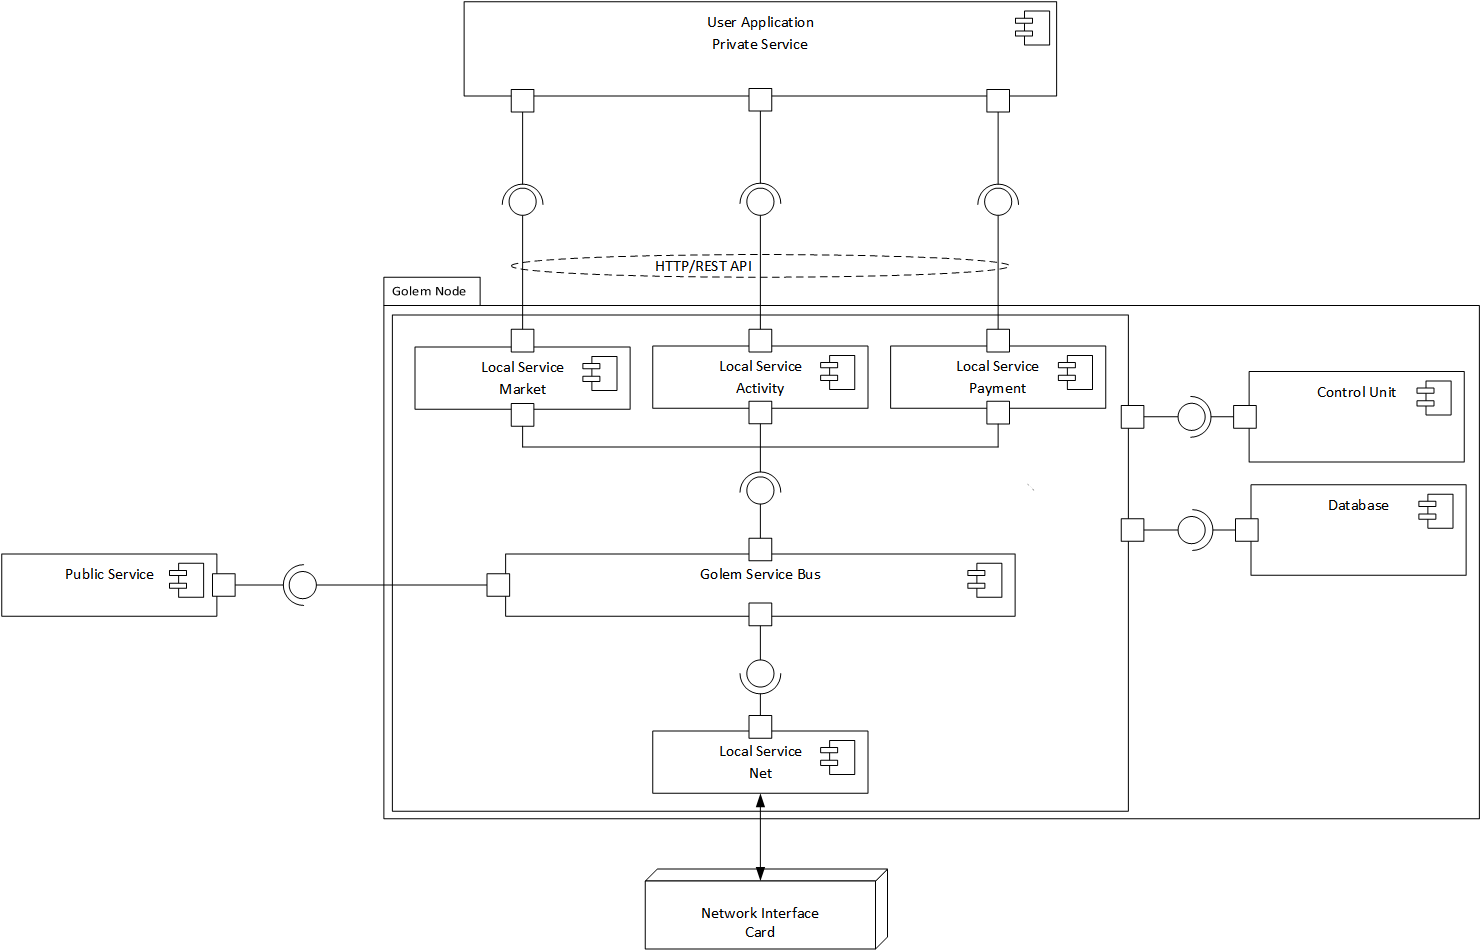
\includegraphics[width=18cm,angle=0]{./diag/Abstract/DetailPackage-Abstract.png}
	\caption{Detail Packages Concept}
    \label{fig:DPC}
\end{figure}


\newpage

The subject of the trade (purchase-sale of the service of using computing resources)
is described using the service model description language (Golem SMDL).
This language is based on a simple definition of resource parameters (the list is available) and their constraints, which are expressed using filters.
The filter syntax is based on the LDAP filter syntax.

The general description of the service should include:

\begin{itemize}
\item {\bf Resource vector R} describes the infrastructure environment using qualitative and quantitative parameters as a service being traded
\item {\bf Usage vector B} defines the factors influencing the measurement of the consumption of the service of using computing resources. These factors are expressed in arbitrary counters
\item {\bf Context vector C} includes important factors that affect the price
\item {\bf Pricing function} indicates the service parameters and cumulative usage counters that affect the cost of the service
\end{itemize}

The following parties participate in the trading process

\begin{itemize}
\item {\bf requestor :} a role of a P2P network node that wants to use the computing resources of other nodes.
\item {\bf provider :} a role of a P2P network node that wants to sell its resources to other nodes
\item {\bf user :} an end user who represents the requestor node and/or the provider
\item {\bf developer :} an application developer
\end{itemize}

A user as a provider prepares an offer in the form of an Offer object using the service model description language.
A user as a requestor prepares a demand in the form of a Demand object using the service model description language.
Both the Offer and Demand objects consist of two elements:

\begin{itemize}
\item properties
\item constraints
\end{itemize}

The formal language of resource description and settlement conditions is intended to automatically or semi-automatically associate demands with offers.
The specification of the service model description language is presented later in the document.

\newpage

%A single aspect of a resource and/or service defines a dimension of the namespace.
% Thus, a set of dimensions creates a multidimensional structure of the namespace.
%Golem Agent contains basic tools for creating a decentralized market of distributed applications and services. These are:
%\begin{enumerate}
%\item {\bf Golem Market Service (GMS)}
%\item {\bf Golem Activity Service (GAS)}
%\item {\bf Golem Payment Service (GPS)}
%\item {\bf Golem Net Service (GNS)
%\item {\bf Golem Services API}
%The following APIs are available:
%\begin{itemize}
%\item Golem Market Service API (GMS API)
%\item Golem Activity Service API (GAS API)
%\item Golem Payment Service API (GPS API)
%\item Golem Net Service API (GNS API)
%\item Golem Service Bus API (GSB API)
%\end{itemize}
%All of the above services have APIs that allow you to create new decentralized and distributed applications and services,
%which use the created Golem network infrastructure (Gntw) and the genericity properties of the underlying services.
%The APIs of individual services also allow you to create interaction automation, e.g. settlements, 
%and offer optimization and orders, and many other tools.
%\end{enumerate}

%\break

%\subsection{Reference Architecture}

%\section{Golem Plane}
\section{Golem Plane}

\subsection{Introduction}

On the Golem Plane (GP) are embedded nodes (GN) that communicate with each other using the P2P protocol, creating the Golem Network.
Each node is built on the basis of the Golem Agent (GA (Yagna)). This component consists of:

\begin{itemize}

\item Golem Toolkit (GTK): A set of REST APIs for creating decentralized and distributed applications and services based on the Golem trade model.

\item Golem Local Services (GLS): A set of basic services available within the node. These are:

\begin{itemize}

\item Golem Market Service (GMS): A service that enables the circulation of offers and demands for computational resources.
The purpose of the circulation is to conclude an agreement between the requestor and the provider of computational resources.

\item Golem Activity Service (GAS) : A service that allows for controlled remote launch of the applicant's application on the supplier's computing resources, 
in accordance with the concluded agreement.

\item Golem Payment Service (GPS) : A service that allows for the settlement of the executed agreement between the requestor and the provider 
via a selected payment platform.

\item Golem Net Service (GNS) : A service that manages communication between Golem nodes via P2P protocols.

\end{itemize}

\item Golem Agent Console (GAC) : A Command Line Interface (CLI) used to configure, monitor applications and services on the Golem Agent component.

\item Golem Public Services (GPuS) : A set of services available from other nodes and/or networks.

\item Golem Database (GDB) : An element of the Golem Agent component that allows for recording transactions to the embedded database.

\item Golem Service Bus (GSB) : A Golem Agent component element that enables communication between the binded Golem Local and Public Services.

\item Golem Agent Daemon (GAD) : A module that works as a background process and handles the Golem Agent component elements.

\end{itemize}

\break
\newpage

\subsection{Golem Network}

\subsubsection{Introduction}




\subsubsection{Golem Node}



\subsubsubsection{Golem Agent}

\subsubsubsection{Golem Agent Console}

\subsubsubsection{Golem Service Bus}


%\subsubsubsubsection{Golem Net Point}
%\subsubsubsubsection{Golem Market Point}
%\subsubsubsubsection{Golem Activity Point}
%\subsubsubsubsection{Golem Payment Point}
%\subsubsubsection{Golem Abstraction Resource}
%\subsubsubsubsection{Physical Resource}
%\subsubsubsubsection{Golem Resource Point}

\subsubsubsection{Golem Services}

\subsubsubsubsection{Golem Net Service}

In a single node, the above services communicate with each other via the Golem Service Bus (GSB).
In turn, communication between nodes takes place via the Golem Net Service (GNS) service, which provides Peer2Peer (P2P) protocols.

%This service also provides communication to the Registry and Discovery Service located on the Golem Central Net Server (GCNS).

Figure ~\ref{fig:SCR} on page ~\pageref{fig:SCR}).

\begin{figure}[H]
    \centering
    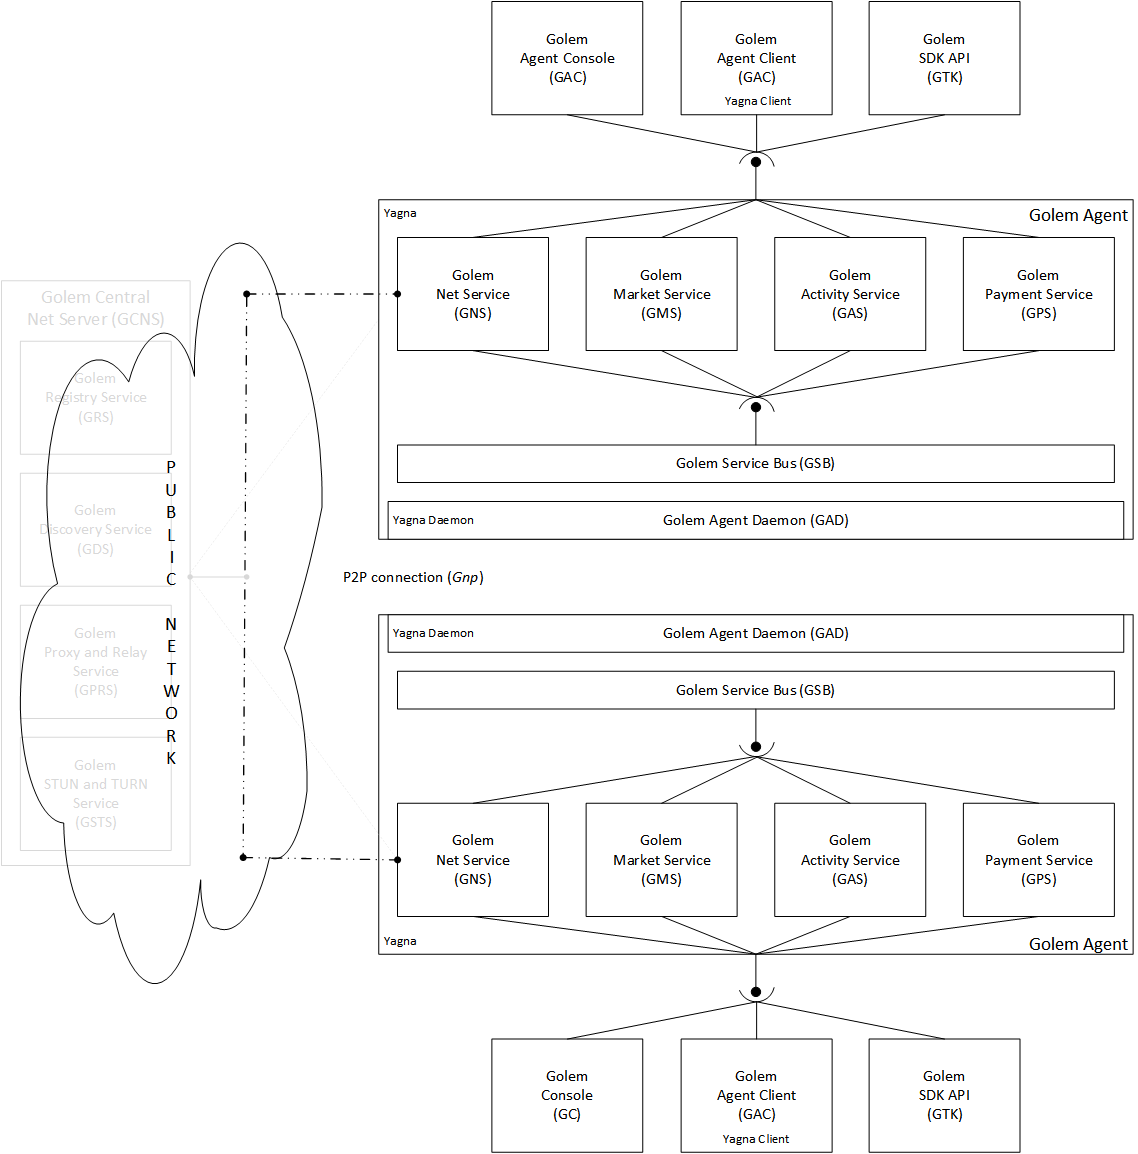
\includegraphics[width=12cm,angle=0]{./diag/Reference/ServicesConcept-Reference.png}
	\caption{Intra and Inter Communication between Services in Nodes}
    \label{fig:SCR}
\end{figure}


In a single node, the above services communicate with each other via the Golem Service Bus (GSB), the so-called Intra Connection.
In turn, communication between nodes takes place via the Golem Net Service (GNS), which provides Peer2Peer (P2P) protocols, the so-called Inter Connection.
Golem Net Service provides the following communication models

\begin{enumerate}

\item Model Mrk0: CentraNet Proxy

\begin{enumerate}

\item Assumptions

\begin{itemize}

\item Ease of implementation
\item Must be able to penetrate Firewall above
\item Does not have to be efficient
\item Does not have to be decentralized
\item Does not have to support End2End pinging

\end{itemize}

\item Limitation

\item Flow

(Please see Figure ~\ref{fig:MM0C} on page ~\pageref{fig:MM0C}).

\begin{figure}[H]
    \centering
    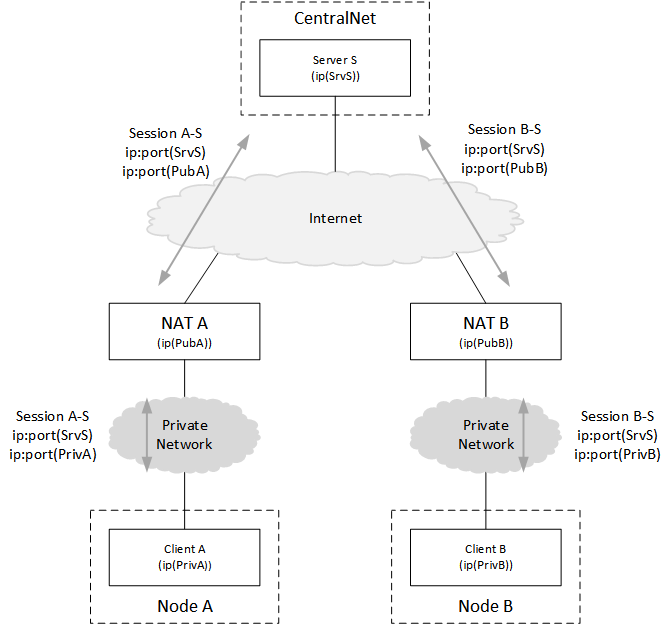
\includegraphics[width=7cm,angle=0]{./diag/Issue/NATRelaying-Mk0-Issue.png}
	\caption{Model Mrk0 Communication}
    \label{fig:MM0C}
\end{figure}

\item Stack

\item Sequence Diagram

\end{enumerate}

\item Model Mrk1: P2P Hybrid

Hybrid P2P networks combine elements of decentralized and centralized architectures.
The CentralNet server plays the role of managing node registration and discovery.
Hybrid P2P networks aim to achieve a balance between decentralization and efficiency.

\begin{enumerate}

\item Assumptions

\begin{itemize}

\item CentralNet Server with registration and discovery nodes service.

\item ability to send small amount of data to other nodes, about 300 kb per minute

\item if a node has a publicly available tcp/udp port, it can ask other nodes to connect,
using the ability to send data through the central server.

\item if nodes do not have publicly available tcp/udp port they can use central net to coordinate NAT hole punching
If nodes does not have publicly available tcp / udp port they can use central net to coordinate NAT hole punching

\item discovery service accepts unencrypted UDP/TCP communication.

\item in the distant future websocket / https://webrtc.rs/ - for browser compatibility.

\end{itemize} 

\item Limitation 

\item Flow

TODO Description

(Please see Figure ~\ref{fig:MM1C} on page ~\pageref{fig:MM1C}).

\begin{figure}[H]
    \centering
    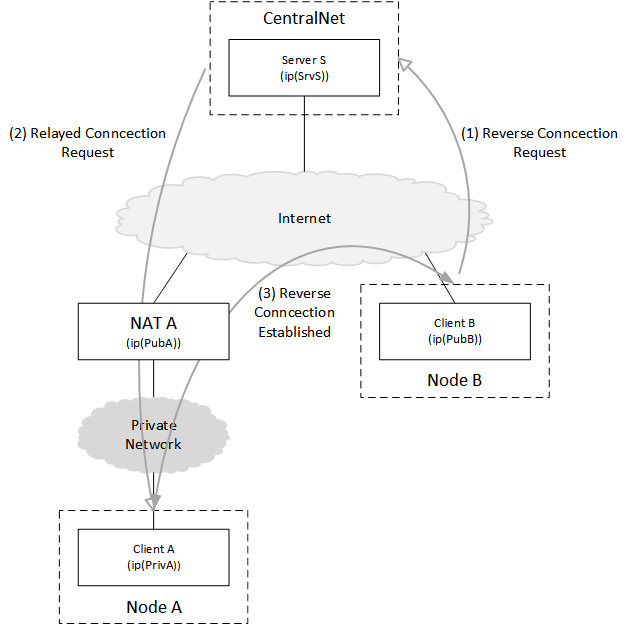
\includegraphics[width=7cm,angle=0]{./diag/Issue/NATReversal-Mk1-Issue.png}
	\caption{Model Mrk1 Communication}
    \label{fig:MM1C}
\end{figure}

\item Stack

TODO Description

(Please see Figure ~\ref{fig:M1PL} on page ~\pageref{fig:M1PL}).

\begin{figure}[H]
    \centering
    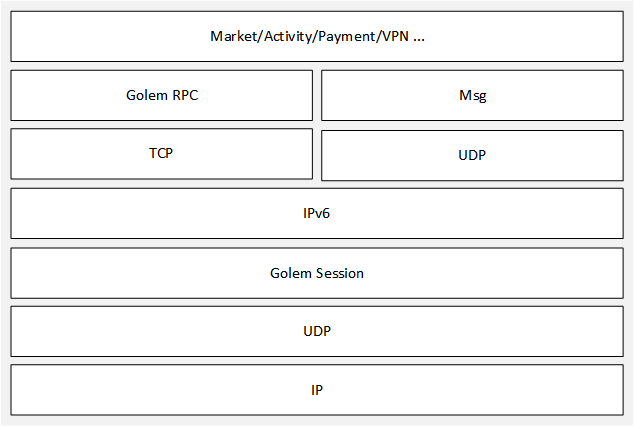
\includegraphics[width=10cm,angle=0]{./diag/Issue/NetBlock-Mk1-Issue.png}
	\caption{Protocol Mrk1 Layers}
    \label{fig:M1PL}
\end{figure}

\break

\item Sequence Diagram

TODO Description

(Please see Figure ~\ref{fig:M1SN} on page ~\pageref{fig:M1SN}).

\begin{figure}[H]
    \centering
    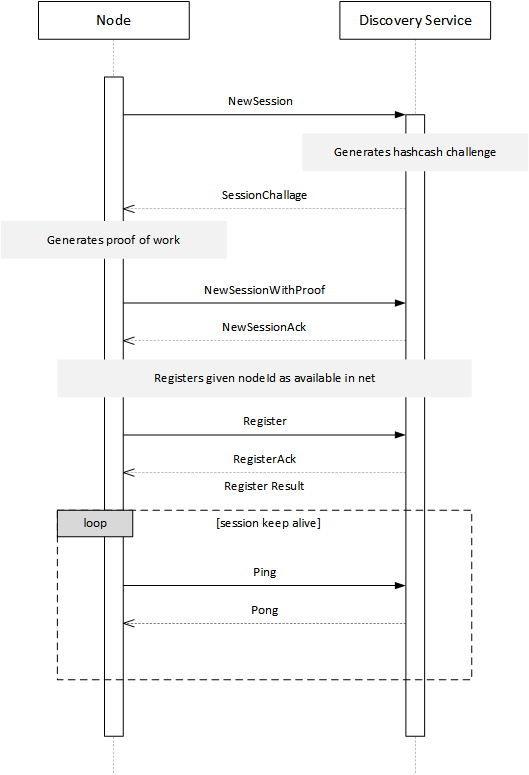
\includegraphics[width=8cm,angle=0]{./diag/Issue/SessionNegotiation-Mk1-Issue.png}
	\caption{Mrk1 Session Negotiation}
    \label{fig:M1SN}
\end{figure}


\end{enumerate} 

\item Model Mrk2: WebRTC 

\begin{enumerate} 
\item Assumptions 
\item Limitation 
\item Flow
\item Stack
\item Sequence Diagram
\end{enumerate} 

\end{enumerate}

In the Golem system, in the Net service, tuples are used to describe objects such as:
node, connection, network, status, address . (Please see Figure ~\ref{fig:NF1} on page ~\pageref{fig:NF1})

TODO figure soon

\begin{enumerate}

\item Node Objects

\begin{enumerate}

\item Object Description

TODO !!

\item Object Fields

\begin{table}[H]
\footnotesize
\begin{center}
\begin{tabular}{|p{3cm}|l|p{3cm}|p{3cm}|p{4cm}|} 
\hline
\rowcolor{lightgray}	Name	& MO.	& Type	& Example & 	Description \\
\hline

id 	& M & string & 		& Node Identifier \\
\hline 		

ip & M & string  & 		& IP address \\
\hline

\end{tabular}
\end{center}
\end{table}

\item Object State

Stateless object

\end{enumerate}

\item Connection Object

\begin{enumerate}

\item Object Description

TODO !!

\item Object Fields

\begin{table}[H]
\footnotesize
\begin{center}
\begin{tabular}{|p{3cm}|l|p{3cm}|p{3cm}|p{4cm}|} 
\hline
\rowcolor{lightgray}	Name	& MO.	& Type	& Example & 	Description \\
\hline

protocol 		& M & integer & 11		&  \\
\hline 		

localIp 		& M & string  & 0.0.0.0	& Local IP address v4 or v6 \\
\hline

localPort 		& M & integer & 1234	& Local Port \\
\hline 

remoteIp 		& M & string  & 0.0.0.0	& Local IP address v4 or v6 \\
\hline

remotePort 		& M & integer & 4321	& Local Port \\
\hline 

\end{tabular}
\end{center}

\end{table}

\item Object State

Stateless object

\end{enumerate}


\end{enumerate}

\break

\subsubsubsubsection{Golem Market Service}

This service has functions for creating a market of distributed computing resources.
This service allows sellers (Providers) to describe the subject of sale in the form of an offer
and buyers (Requestors) to describe the subject of demand in the form of a Demand.

In addition, the service allows for decentralized searches of offers and demands in order to associate them
based on the conditions described in offers and demands. Matched objects are represented as
proposal. An accepted and confirmed proposal allows for the creation of an agreement object, which
after being signed by the parties is a confirmation of the sale and purchase of goods such as computing resources.

The Market service is based on the tuple space (Tuples Space).
A tuple is a finite list of elements that can be used to represent a data item or a message.

In the Golem system, in the Market service, tuples are used to describe objects such as:
offer, demand, proposal, agreement. (Please see Figure ~\ref{fig:MF1} on page ~\pageref{fig:MF1}
and Figure ~\ref{fig:MF2} on page ~\pageref{fig:MF2}).

\begin{figure}[H]
    \centering
    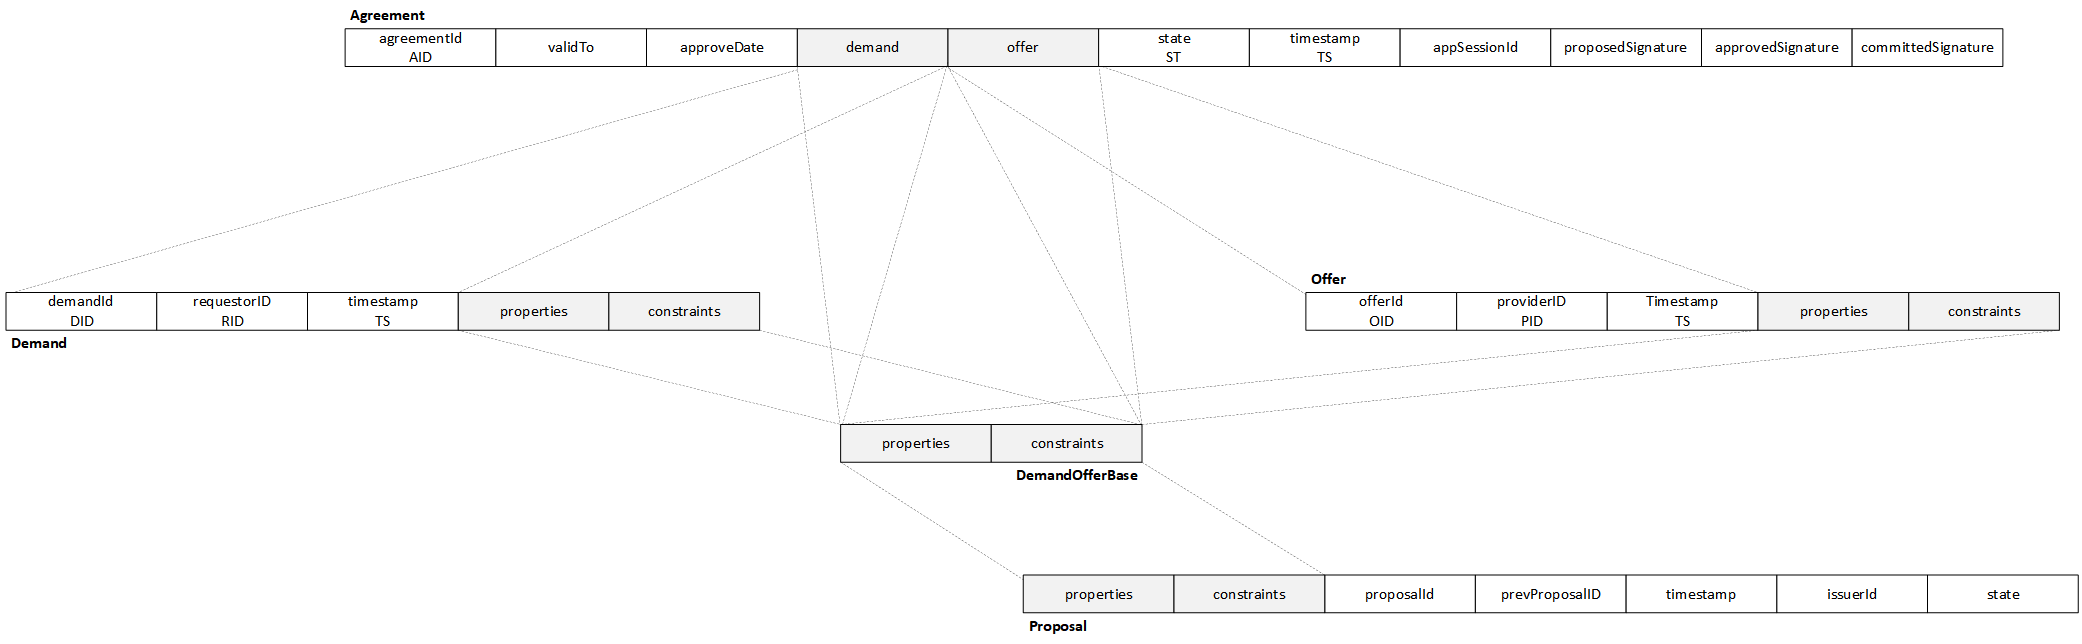
\includegraphics[width=18cm,angle=0]{./diag/Reference/MarketFrame-1-Reference.png}
	\caption{Market Objects Frame}
    \label{fig:MF1}
\end{figure}


\begin{figure}[H]
    \centering
    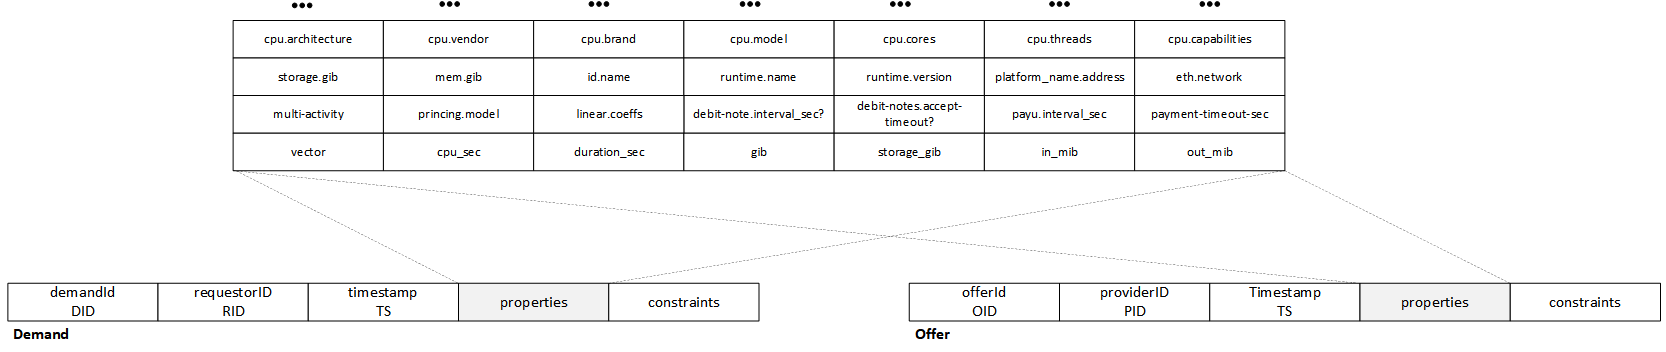
\includegraphics[width=16cm,angle=0]{./diag/Reference/MarketFrame-2-Reference.png}
	\caption{Market Objects Frame}
    \label{fig:MF2}
\end{figure}

\begin{enumerate}

\item Offer Objects

\begin{enumerate}

\item Object Description

Offer is created by Provider nodes and contains the description of the
computing resources the node has to offer, as well as any optional conditions
for their use (e.g. limiting their availability only to certain requestor nodes).

\item Object Fields

\begin{table}[H]
\footnotesize

\begin{center}
\begin{tabular}{|p{3cm}|l|p{3cm}|p{3cm}|p{4cm}|} 
\hline
\rowcolor{lightgray}	Name	& MO.	& Type	& Example & 	Description \\
\hline

offerId 	& M & string & 		& Offer Identifier \\
\hline 		

providerId & M & string  & 		& Provider Node Identifier \\
\hline

timestamp	& M	& 	string(\$date-time)	& YYYY-MM-DDThh:mm:ss.sssZ	&	Time of ???  \\
\hline

properties	& M	& 	json or flat	&		&	Offer properties \\ 
\hline

constraints	& M	& 	string	&		&	Offer constraints \\ 
\hline

\end{tabular}
\end{center}

\end{table}

\item Object State

Stateless object

\end{enumerate}

\item Demand Objects

\begin{enumerate}

\item Object Description

Demand is created by Requestor nodes and contains description of the
payload, including properties telling what capabilities the payload might
require (e.g. specific hardware architecture or features) and optionally other
conditions which ought to be satisfied by the provider nodes (e.g. asking only
for nodes which are located within specific country). 

%	Most of the content of the Demand is opaque for the Golem network

\item Object Fields

\begin{table}[H]
\footnotesize

\begin{center}
\begin{tabular}{|p{3cm}|l|p{3cm}|p{3cm}|p{4cm}|} 
\hline
\rowcolor{lightgray}	Name	& MO.	& Type	& Example & 	Description \\
\hline

demandId 	& M & string  & 		& Demand Identifier \\
\hline 		

requestorId & M & string  & 		& Requestor Node Identifier \\
\hline

timestamp	& M	& 	string(\$date-time)	& YYYY-MM-DDThh:mm:ss.sssZ	&	Time of ???  \\
\hline

properties	& M	& 	json or flat	&		&	Demand properties \\ 
\hline

constraints	& M	& 	string	&		&	Demand constraints \\ 
\hline

\end{tabular}
\end{center}
\end{table}

\item Object State

Stateless object

\end{enumerate}

\item Proposal Objects

\begin{enumerate}

\item Object Description

A proposal (Proposal object) is a Demand-Offer pair (DemandOfferBase object), with a proposalId identifier and status
and a set of field elements that allow handling of the Negotiation operation. These are: the identifier of the node submitting the proposal,
the time the proposal was created, the identifier of the proposal from the other side, to which this proposal responds.

\item Object Fields

\begin{table}[H]
\footnotesize

\begin{center}
\begin{tabular}{|p{3cm}|l|p{3cm}|p{3cm}|p{4cm}|} 
\hline
\rowcolor{lightgray}	Name	& MO.	& Type	& Example & 	Description \\
\hline

properties		& M	& 	json or flat		&												&	Proposal properties \\ 
\hline

constraints		& M	& 	string				&												&	Proposal constraints \\ 
\hline

proposalId		& M & 	string  			& 												& 	Proposal Identifier \\
\hline

issuerId		& M & 	string				&												& 	Issuer Node Identifier 	\\ 
\hline

state			& M & 	string(enum) 		& [Initial, Draft, Rejected, Accepted, Expired]	&  Proposal State	\\
\hline

timestamp		& M	& 	string(\$date-time)	& YYYY-MM-DDThh:mm:ss.sssZ						&	Time of ???  \\
\hline

prevProposalId 	& O & 	string				&												& 	Id of the Proposal from other side which this proposal responds to \\
\hline

\end{tabular}
\end{center}
\end{table}

\item Object State

(Please see Figure ~\ref{fig:PSD} on page ~\pageref{fig:PSD}).

\begin{figure}[H]
    \centering
    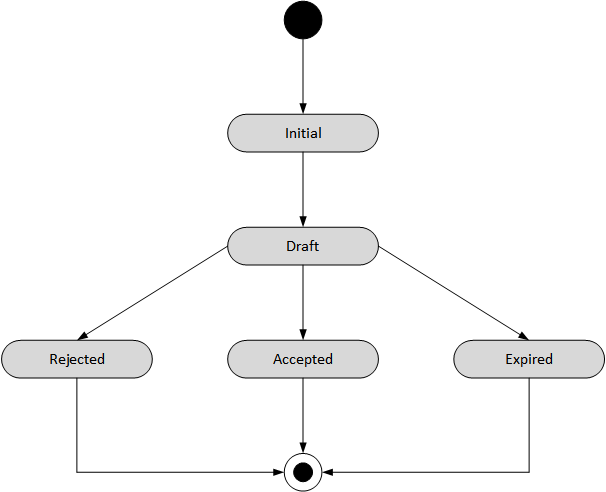
\includegraphics[width=7cm,angle=0]{./diag/Reference/ProposalState-Reference.png}
	\caption{Proposal State Diagram}
    \label{fig:PSD}
\end{figure}

\begin{table}[H]
\footnotesize

\begin{center}
\begin{tabular}{|p{3cm}|p{11cm}|} 
\hline
\rowcolor{lightgray}	State	& 	Description \\
\hline

Initial 	&	proposal arrived from the market as response to subscription \\
\hline
Draft 		&	bespoke counter-proposal issued by one party directly to other party (negotiation phase) \\
\hline
Rejected 	&	reject by other party \\
\hline
Accepted 	&	promoted into the Agreement draft \\
\hline
Expired 	&	not accepted nor rejected before validity period \\
\hline

\end{tabular}
\end{center}
\end{table}

\end{enumerate}

\item Agreement Objects

\begin{enumerate}

\item Object Description

The Agreement object is a set of basic terms of the agreement between two parties establishing their mutual relations
in relation to the subject of the service in the market space.
The basic terms of the agreement are:

\begin{itemize}

\item Established and confirmed terms of the proposal (Proposal object) within the Negotiation operation

\item Agreement object identifier

\item Agreement object state

\item Validity date of the Agreement object circulation between the parties

\item Agreement object approval date

\item Agreement object creation date

\item Correlation/session identifier used to search for events related to the action ???

\item Proposed signature

\item Confirmed signature

\item Approved signature

\end{itemize}

\item Object Fields

\begin{table}[H]
\footnotesize

\begin{center}
\begin{tabular}{|p{3cm}|l|p{3cm}|p{3cm}|p{4cm}|} 
\hline
\rowcolor{lightgray}	Name	& MO.	& Type	& Example & 	Description \\
\hline

agreementId			& M & string 				&				& 	Agreement Identifier \\
\hline

demand				& M	& object 				&				& 	Demand		\\
\hline

offer 				& M & object 				& 				& 	Offer 		\\
\hline

validTo				& M & string(\$date-time)	& YYYY-MM-DDThh:mm:ss.sssZ & End of validity period. 
																			Agreement needs to be approved, rejected or cancelled before this date; 
																			otherwise will expire. \\
\hline

approveDate			& M & string(\$date-time)	& YYYY-MM-DDThh:mm:ss.sssZ & Agreement approval timestamp \\
\hline

state 				& M & string(enum) 				&[Proposal, Pending, Cancelled, Rejected, Approved, Expired, Terminated] & Agreement State \\
\hline

timestamp			& M	& 	string(\$date-time)	& YYYY-MM-DDThh:mm:ss.sssZ	&	Time of ???  \\
\hline

appSessionId		& O &	string 				&							& 	A correlation/session identifier used for querying events related to an action 
																				where this appSessionId has been specified		\\
\hline

proposedSignature 	& O & 	string 				&							&			\\
\hline

approvedSignature 	& O & 	string 				& 							&			\\
\hline

committedSignature	& O &	string 				& 							& 			\\
\hline

\end{tabular}
\end{center}
\end{table}

\item Object State

(Please see Figure ~\ref{fig:ASD} on page ~\pageref{fig:ASD}).

\begin{figure}[H]
    \centering
    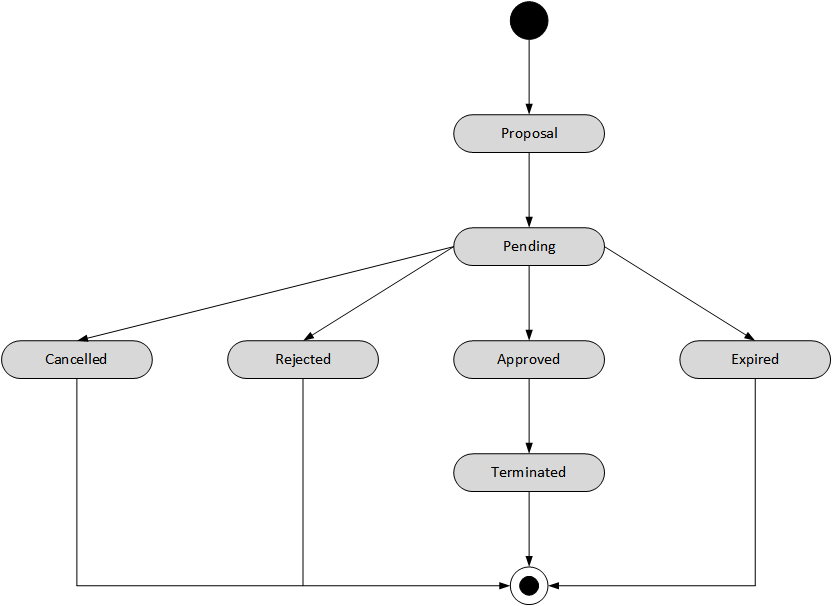
\includegraphics[width=9cm,angle=0]{./diag/Reference/AgreementState-Reference.png}
	\caption{Agreement State Diagram}
    \label{fig:ASD}
\end{figure}

\begin{table}[H]
\footnotesize

\begin{center}
\begin{tabular}{|p{3cm}|p{11cm}|} 
\hline
\rowcolor{lightgray}	State	& 	Description \\
\hline

Proposal	&	newly created by a Requestor (draft based on Proposal) \\
\hline
Pending		&	confirmed by a Requestor and send to Provider for approval \\
\hline
Cancelled 	& 	by a Requestor \\
\hline
Rejected 	&	by a Provider \\
\hline
Approved 	&	by both sides \\
\hline
Expired 	&	not approved, rejected nor cancelled within validity period \\
\hline
Terminated 	&	finished after approval. \\
\hline

\end{tabular}
\end{center}
\end{table}

\end{enumerate}

\item DemandOfferBase Object

\begin{enumerate}

\item Object Description

The DemandOfferBase object is a temporary object that collects negotiated terms related to the service item.

\item Object Fields

\begin{table}[H]
\footnotesize

\begin{center}
\begin{tabular}{|p{3cm}|l|p{3cm}|p{3cm}|p{4cm}|} 
\hline
\rowcolor{lightgray}	Name	& MO.	& Type	& Example & 	Description \\
\hline

properties	& M	& 	json or flat	&		&  Temporary Proposal properties \\ 

\hline

constraints	& M	& 	string	&		&	Temporary Proposal constraints \\ 

\hline

\end{tabular}
\end{center}
\end{table}

\item Object State

Stateless object

\end{enumerate}

\end{enumerate}

\break

The Market Space is used to define interaction operations on these objects such as:

\begin{enumerate}
\item  Observation Operation

\begin{enumerate}

\item Description

The Market Observation operation is implemented by a set of Scan functions. 
These functions, together with REST API methods, allow to aggregate data from currently circulating 
offers (Offer object) and demands (Demand object).

The BeginScan() function initiates the scanning operation by accepting the filtering criteria and 
returning scanId. The results are aggregated and collected by the CollectScanResults() function.
The EndScan() function closes the data aggregation process.

The criteria for searching the Golem network market are defined using the service model description language (Golem SMDL),
where the filter syntax is based on the LDAP filter syntax. Depending on the needs, simple or complex search criteria can be defined.

(Please see Figure ~\ref{fig:MOO} on page ~\pageref{fig:MOO}).

\item Sequence Diagram

\begin{figure}[H]
    \centering
    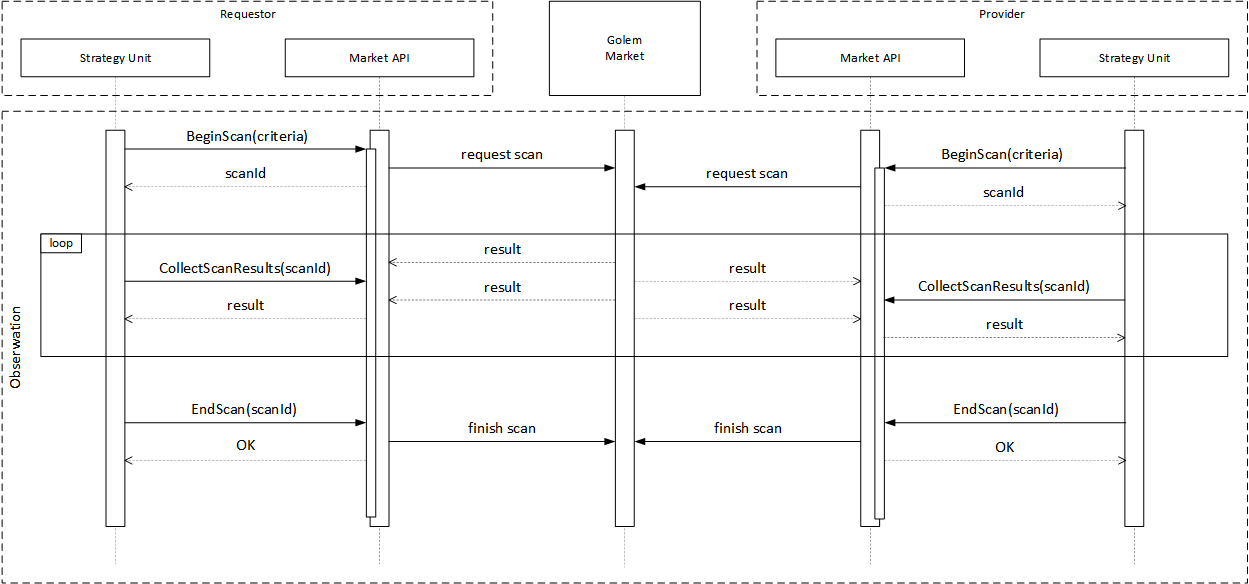
\includegraphics[width=14cm,angle=0]{./diag/Sequence/MarketObservation-B-Sequence.png}
	\caption{Market Observation Operation}
    \label{fig:MOO}
\end{figure}

\item Functions and Methods

\begin{table}[H]
\footnotesize

\begin{center}
\begin{tabular}{|p{3cm}|p{7cm}|p{1.5cm}|p{4cm}|} 
\hline
\rowcolor{lightgray}	Function Name	& API Method Name	& 	Side	&	Description \\
\hline

BeginScan 				& POST /scan								&	Both	&	\\
\hline

CollectScanResult		& GET /scan/\{subscriptionId\}/events		&	Both 	& ?? subscriptionId or scanId ??	\\
\hline

EndScan 				& DELETE /scan/\{subscriptionId\}/events	&	Both 	& ?? subscriptionId or scanId ??	\\
\hline

\end{tabular}
\end{center}
\end{table}

\end{enumerate}

\item  Discovery Operation

\begin{enumerate}

\item Description

The Discovery operation is implemented by a set of Subscribe functions. These functions, together with REST API methods, 
allow for the aggregation of data from currently circulating active offers (Offer object) and active demands (Demand object).

The Subscribe() function publishes the offer (Offer object) and demand (Demand object) on the Golem Network Market, respectively.
The aggregated results in the form of proposals (Proposal object) with matching Demand-Offer pairs are collected by the Collect() function.
The Unsubscribe() function disables the availability of offers and demands on the Golem Network Market.

The Discovery operation is the only one that involves indirect communication (e.g. via a P2P network).
The subsequent phases are direct (one-to-one)

(Please see Figure ~\ref{fig:MDO} on page ~\pageref{fig:MDO}).

\item Sequence Diagram

\begin{figure}[H]
    \centering
    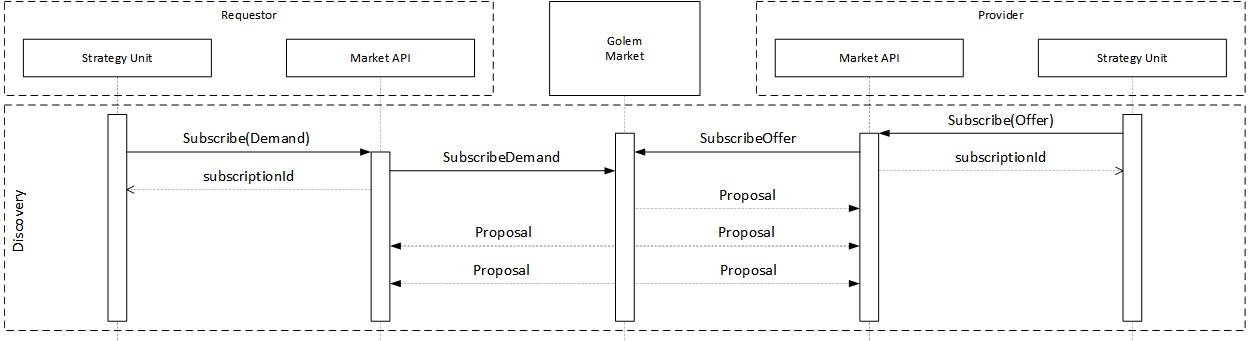
\includegraphics[width=14cm,angle=0]{./diag/Sequence/MarketDiscovery-B-Sequence.png}
	\caption{Market Discovery Operation}
    \label{fig:MDO}
\end{figure}

\item Functions and Methods

\begin{table}[H]
\footnotesize

\begin{center}
\begin{tabular}{|p{3cm}|p{7cm}|p{1.5cm}|p{4cm}|} 
\hline
\rowcolor{lightgray}	Function Name	& API Method Name	& 	Side	&	Description \\
\hline

Subscribe			&	POST /offers							&	Provider	&	Publishes Provider capabilities via Offer \\
\hline

Subscribe			&	POST /demands							& 	Requestor	&	Publishes Requestor capabilities via Demand \\
\hline

Unsubscribe			&	DELETE	/offers/\{subscriptionId\}		&	Provider	&	Stop subscription for published Offer \\
\hline

Unsubscribe			&	DELETE	/demands/\{subscriptionId\}		&	Requestor	&	Stop subscription for published Demand \\
\hline	 

CollectDemands ?	&	GET	/offers/\{subscriptionId\}/events	&	Provider &	Reads Market responses to published Offer \\
\hline

CollectOffers ?		&	GET	/demands/\{subscriptionId\}/events	&	Requestor &	Reads Market responses to published Demand \\
\hline

Collect				& 	POST /offers/\{subscriptionId\}/ \newline propertyQuery/\{queryId\} & Provider & Handles dynamic property query \\
\hline

Collect				& 	POST /demands/\{subscriptionId\}/ \newline propertyQuery/\{queryId\} & Requestor & Handles dynamic property query \\
\hline 

					&	GET /offers								&	Provider	&	Fetches all active Offers which have been published by the Provider \\
\hline

					&	GET /demands							& 	Requestor	&	Fetches all active Demands which have been published by the Requestor \\
\hline	 

\end{tabular}
\end{center}
\end{table}

\end{enumerate}

\item  Negotiation Operation

\begin{enumerate}

\item Description

The Negotiation operation is implemented by a set of REST API functions and methods that allow for reaching a consensus between the parties
by matching offers and demands. This is done by automatic or semi-automatic exchange of documents (Offer and Demand objects)
between the parties in the form of proposals (Proposal object). 
The negotiation conditions are described by the service model description language (Golem SMDL) 
where the filter syntax is based on the LDAP filter syntax.

The Collect() function collects aggregated results in the form of proposals (Proposal object) from the data contained 
in the offer (Offer object) and in the demand (Demand object).

The CounterProposal() function In the case of the Requestor node, it creates and sends a modified version of the original demand 
(Demand object as a counterproposal) adapted to the previously received Proposal (i.e. Offer).
In the case of the Provider node, it creates and sends a modified version of the original offer (the Offer object as a counterproposal) 
adapted to the previously received proposal (i.e. Demand). The function for both cases changes the state of the Proposal object to Draft 
and returns the created proposalId. 

The RejectProposal() function effectively ends the negotiation chain - it clearly indicates
that the sender will not create another counterproposal. If the negotiations reach a consensus, 
then an agreement (the Agreement object) is generated by the CreateAgreement() function of the Agreement operation. 

The Provider node retrieves the proposal (Demand) with the given proposalId using the GetProposalDemand() method. 
The Requestor node retrieves the proposal (Offer) with the given proposalId using the GetProposalOffer() method.

(Please see Figure ~\ref{fig:MNO} on page ~\pageref{fig:MNO}).

\item Sequence Diagram

\begin{figure}[H]
    \centering
    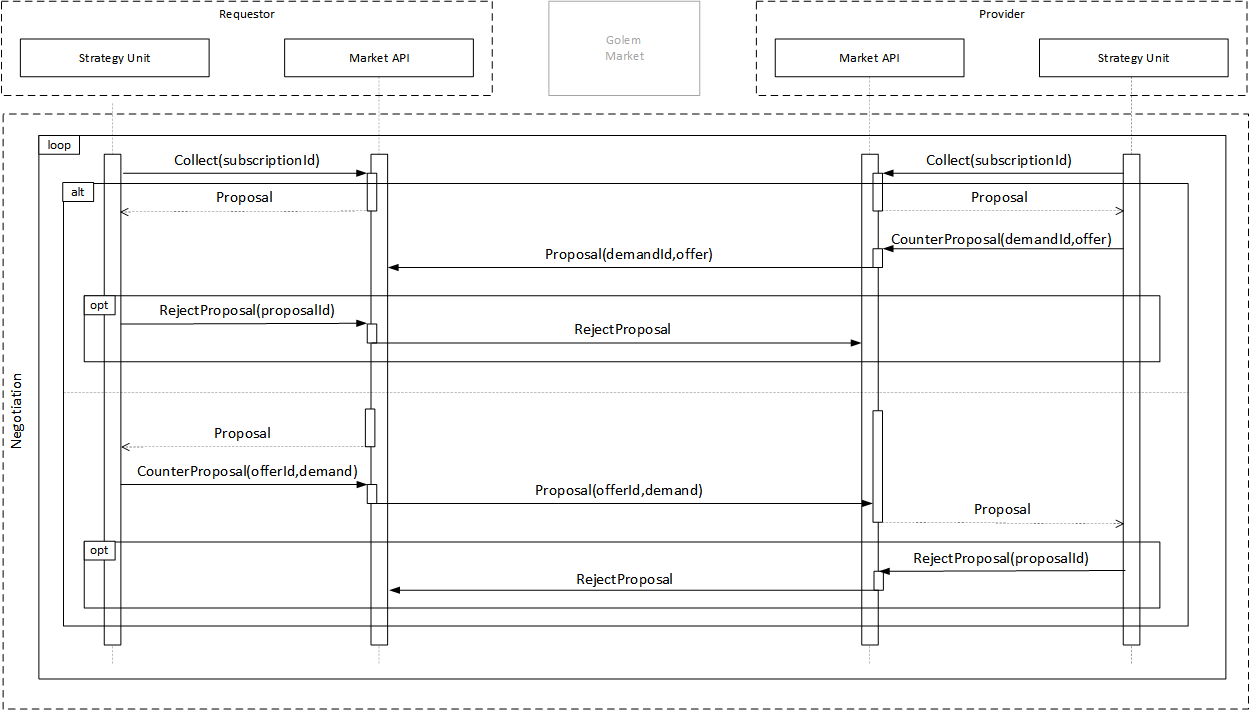
\includegraphics[width=14cm,angle=0]{./diag/Sequence/MarketNegotiation-B-Sequence.png}
	\caption{Market Negotiation Operation}
    \label{fig:MNO}
\end{figure}

\item Functions and Methods

\begin{table}[H]
\footnotesize

\begin{center}
\begin{tabular}{|p{3cm}|p{7cm}|p{1.5cm}|p{4cm}|} 
\hline
\rowcolor{lightgray}	Function Name	& API Method Name	& 	Side	&	Description \\
\hline

Collect			&	GET /offers/\{subscriptionId\}/events	&	Provider	&	Reads Market responses to published Offer \\
\hline

Collect			&	GET /demands/\{subscriptionId\}/events	&	Requestor	&	Reads Market responses to published Demand \\
\hline

CounterProposal	&	POST /offers/\{subscriptionId\}/ \newline proposals/\{proposalId\}	&	Provider	&	Responds with a bespoke Offer to received Demand \\
\hline

CounterProposal	&	POST /demands/\{subscriptionId\}/ \newline proposals/\{proposalId\}	&	Requestor	&	Responds with a bespoke Demand to received Offer \\
\hline

RejectProposal	&	POST /offers/\{subscriptionId\}/ \newline proposals/\{proposalId\}/reject & Provider & Reject Proposal Demand \\
\hline

RejectProposal	&	POST /demands/\{subscriptionId\}/ \newline proposals/\{proposalId\}/reject & Requestor & Reject Proposal Offer \\
\hline

				&	GET /offers/\{subscriptionId\}/ \newline proposals/\{proposalId\}	&	Provider	&	Fetches Proposal (Demand) witch given id \\
\hline

				&	GET /demands/\{subscriptionId\}/ \newline proposals/\{proposalId\}	&	Requestor	&	Fetches Proposal (Offer) witch given id \\
\hline

\end{tabular}
\end{center}
\end{table}

\end{enumerate}

\item  Agreement Operation

\begin{enumerate}

\item Description

The Agreement operation is implemented by a set of REST API functions and methods that allow for the finalization of the Negotiation operation by
confirming receipt of the agreement signed by both parties (Agreement object).

The CreateAgreement() function creates an agreement (Agreement object) from the negotiated proposal (Proposal object) by the Requestor node.

The agreement created by the ConfirmAgreement() function is signed with the Applicant's signR key and sent to the Provider.

The RejectAgreement() function is used to interrupt the Agreement operation by the Provider node.

Running the RejectAgreement() function interrupts the Agreement operation, giving the Requestor node the possibility of returning the negotiation operation,
which can send a new proposal (Proposal object).

The CancelAgreement() function is used to interrupt the Agreement operation by the Requestor node.

This is possible only until the Agreement is approved or rejected by the Provider and before it expires.

The WaitForApproval() function is used to set the time to prepare resources to start the calculations as part of the Activity service operation.
This function is initialized by the Requestor node for the Provider node. After the set time has elapsed, the Requestor node can
re-call this function for the same agreement identifier (agreementId).

The ApproveAgreement() function is used to approve the agreement by the Provider node. It is used when the environment with
resources on the Provider node is ready to start the calculations by the Requestor node as part of the Activity service operation.

The TerminateAgreement() function is used to terminate the agreement in the Approved state.
The other party is notified about the decision of the calling party to terminate the "current" agreement. Available for both types of nodes.

The GetTerminateReason method is used to retrieve the reason for termination of the agreement reported during the call to the TerminateAgreement() function. Available for both types of nodes.

The AgreementEvents method is used to collect events related to the agreement (the Agreement object). These are

\begin{itemize}

\item AgreementApprovedEvent : 	indicates that the Agreement has been approved by the Provider.
								The Provider is now ready to accept the request to start the Activity
								as described in the negotiated agreement.
								The corresponding Provider approveAgreement call returns Approved after emitting this event.

\item AgreementRejectedEvent : 	indicates that the Provider has called rejectAgreement, which effectively stops the Agreement negotiation.
								The Applicant can try to return to the Negotiation phase by sending a new Proposal.

\item AgreementCancelledEvent : indicates that the Applicant has called cancelAgreement, which effectively stops the Agreement negotiation.

\item AgreementTerminatedEvent : indicates that the Agreement has been terminated by the specified party (includes a signature).

\end{itemize}

The ListAgreements method is used to retrieve information about agreements. It uses optional filters:

\begin{itemize}

\item state: [Proposal, Pending, Cancelled, Rejected, Approved, Expired, Terminated ]

\item creation date and time

\item application session identifier

\end{itemize}

The GetAgreementContent() function is used to retrieve an agreement (Agreement object) based on a given identifier (agreementId).

The ValidateAgreementContent() function is used to verify an agreement (Agreement object) sent as a byte stream.

(Please see Figure ~\ref{fig:MAO} on page ~\pageref{fig:MAO}).

\item Sequence Diagram

\begin{figure}[H]
    \centering
    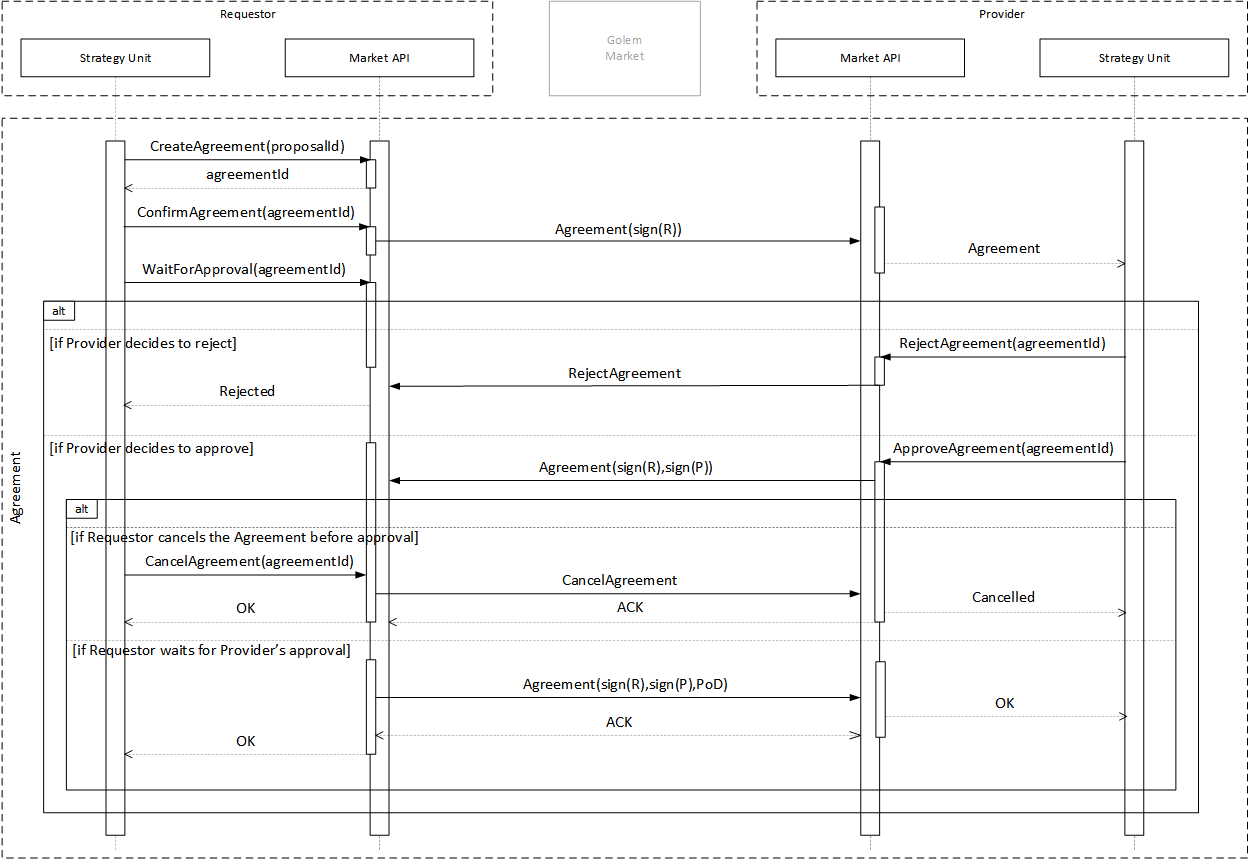
\includegraphics[width=14cm,angle=0]{./diag/Sequence/MarketAgreement-B-Sequence.png}
	\caption{Market Agreement Operation}
    \label{fig:MAO}
\end{figure}

\item Functions and Methods

\begin{table}[H]
\footnotesize

\begin{center}
\begin{tabular}{|p{3cm}|p{7cm}|p{1.5cm}|p{4cm}|} 
\hline
\rowcolor{lightgray}	Function Name	& API Method Name							& 	Side	&	Description \\
\hline

CreateAgreement		&	POST /agreements											& Requestor	&	Creates Agreement from selected Proposal \\
\hline

					&	GET /agreements												&	Both	&	List agreements with optional filters \\
\hline

GetAgreement \newline Content	&	GET /agreements/\{agreementId\}					&	Both	&	Fetches  agreement with agreement id \\
\hline

ValidateAgreement \newline Content &												&	Both	&	Offline function for validation of agreement submitted in the form of byte stream \\
\hline

ConfirmAgreement	& POST /agreements/\{agreementId\}/ \newline terminate			& Requestor & 	Sends Agreement proposal to the Provider \\
\hline

WaitForApproval		& POST /agreements/\{agreementId\}/ \newline wait				& Requestor & 	Waits for Agreement approval by the Provider \\
\hline

CancelAgreement		& POST /agreements/\{agreementId\}/ \newline cancel				& Requestor &	Cancels Agreement	\\
\hline

TerminateAgreement	& POST /agreements/\{agreementId\}/ \newline terminate			& Both		&	Terminates approved Agreement \\
\hline

					& POST /agreements/\{agreementId\}/ \newline terminate/reason 	& Both 		& 	Gets termination reason reported when terminateAgreement operation was called \\
\hline					

					& GET /agreementEvents											& Both 		& 	Collect events related to an Agreement \\
\hline

ApproveAgreement	& POST /agreements/\{agreementId\}/ \newline Approve			& Provider	&	Approves Agreement proposed by the Requestor \\
\hline

RejectAgreement		& POST /agreements/\{agreementId\}/ \newline reject				& Provider	&	Rejects Agreement proposed by the Requestor	\\
\hline

\end{tabular}
\end{center}
\end{table}

\end{enumerate}

\end{enumerate}

%\begin{enumerate}
%    \item Service Profile
%    \item Service Protocol
%    \item Service Interface
%    \item Service Workflow
%\end{enumerate}

\subsubsubsubsection{Golem Activity Service}

This service has tools that allow the Requestor's applications and services to be launched on the Provider's computing resources,
while simultaneously measuring the use of these resources in accordance with the concluded contract in the form of an agreement. 
The measurement of the use of resources is recorded in the form of metrics in the Usage Counters Vector (UCV) object.


\begin{enumerate}
    \item Service Profile
    \item Service Protocol
    \item Service Interface
    \item Service Workflow
\end{enumerate}

\subsubsubsubsection{Golem Payment Service}

This service enables settlements between the parties based on the terms contained in the contract. 
Usage Counters Vector (UCV) objects created in the Golem Activity Service and the settlement terms included in the agreement 
are used to settle the sale-purchase item. The Usage Counters Vector (UCV) associated with the agreement and activity creates 
Activity Detail Record (ADR) objects. Settlement functions allow the ADR object to be transformed into a Debit Note (DN) object, 
where the total incremental settlement amounts for using Provider resources are included. The frequency of creating and sending 
Debit Notes objects between the parties is included in the agreement. The state of completing the use of Provider resources allows 
for the generation of an invoice summarizing the agreement between the parties. 
Payment is made via the blockchain operator. Optimization of payment transaction costs is possible by setting the terms of this operation 
in the agreement object.

In the Golem system, in the Payment service, tuples are used to describe objects such as:
vector usage counters, activity detail record, debit note, invoice . 
(Please see Figure ~\ref{fig:PF1} on page ~\pageref{fig:PF1} and Figure ~\ref{fig:PF2} on page ~\pageref{fig:PF2})

\begin{figure}[H]
    \centering
    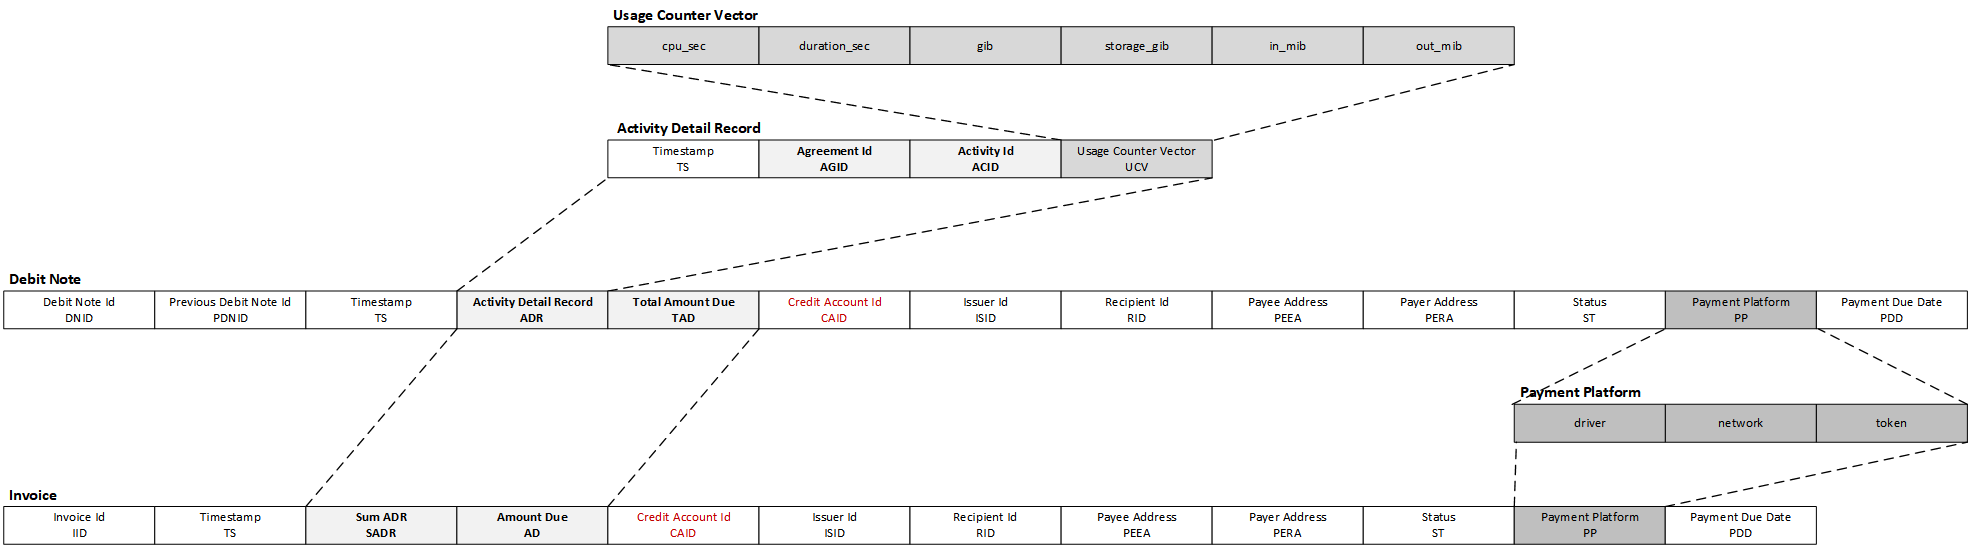
\includegraphics[width=14cm,angle=0]{./diag/Reference/PaymentFrame-1-Reference.png}
	\caption{Debit Note and Invoice Objects Frame}
    \label{fig:PF1}
\end{figure}

\begin{figure}[H]
    \centering
    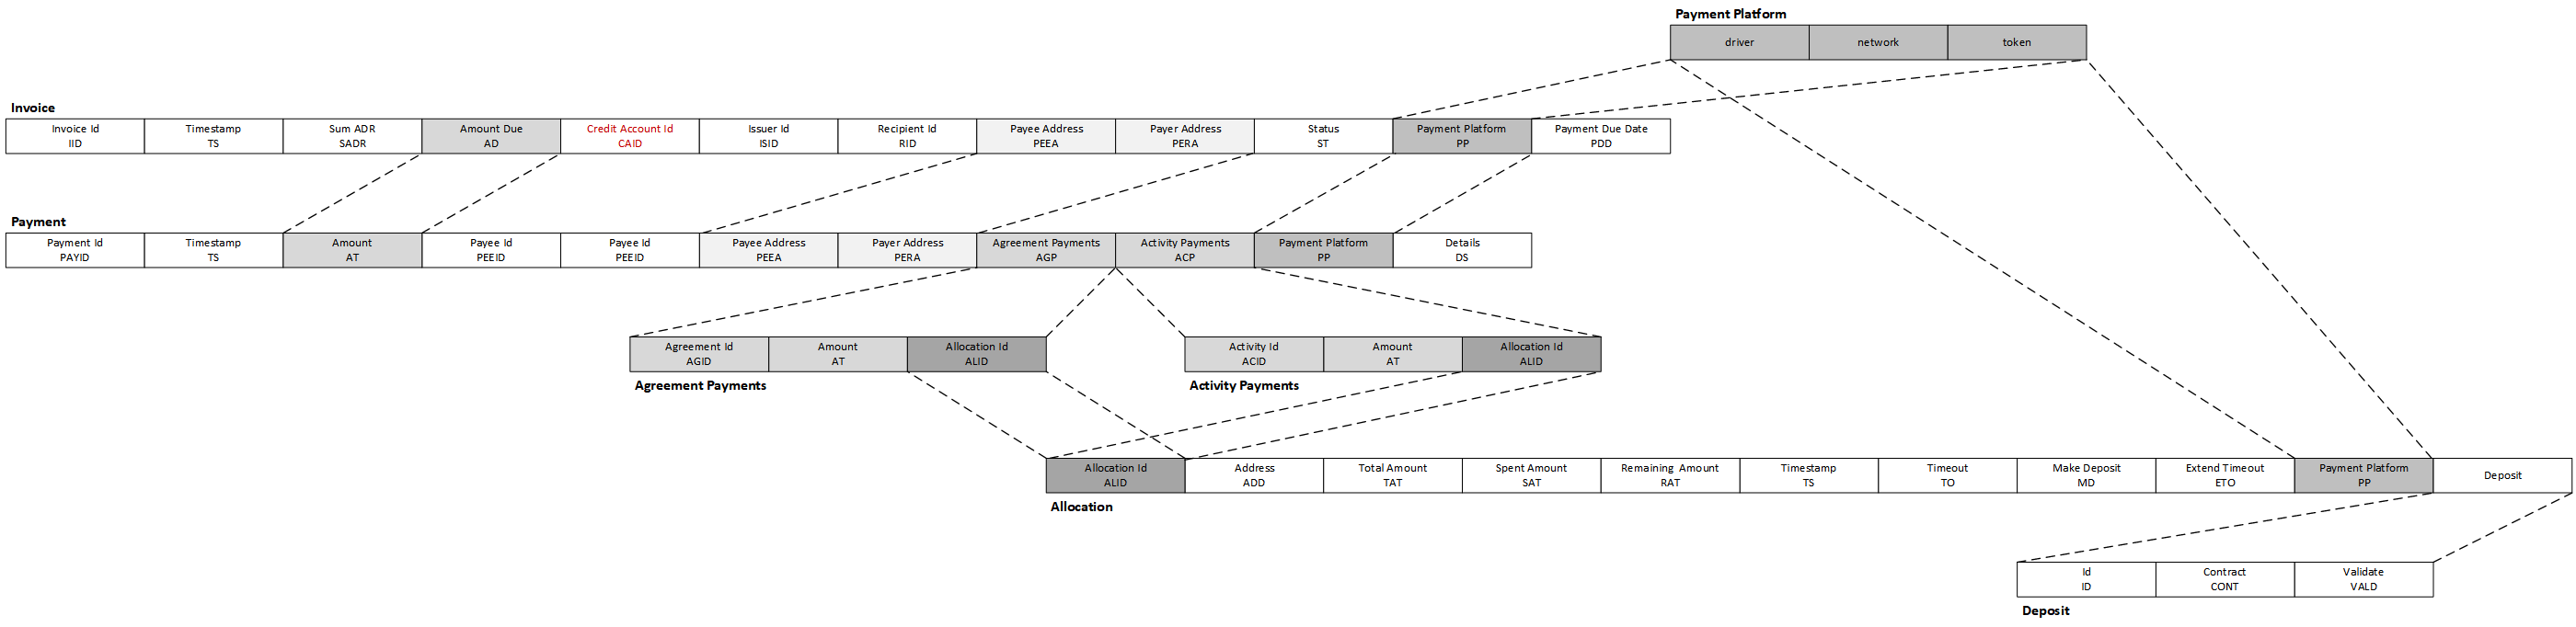
\includegraphics[width=17cm,angle=0]{./diag/Reference/PaymentFrame-2-Reference.png}
	\caption{Payment Objects Frame}
    \label{fig:PF2}
\end{figure}

\begin{enumerate}

\item Usage Counter Vector Objects

\begin{enumerate}

\item Object Description

TODO !!

\item Object Fields

\begin{table}[H]
\footnotesize

\begin{center}
\begin{tabular}{|p{3cm}|l|p{3cm}|p{3cm}|p{4cm}|} 
\hline
\rowcolor{lightgray}	Name	& MO.	& Type	& Example & 	Description \\
\hline

{\it counter} 	& O & string & cpu\_sec		& Counter \\
\hline 		

\end{tabular}
\end{center}
\end{table}

\item Object State

Stateless object

\end{enumerate}

\item Activity Detail Record

\begin{enumerate}

\item Object Description

TODO !!

\item Object Fields

\begin{table}[H]
\footnotesize

\begin{center}
\begin{tabular}{|p{3cm}|l|p{3cm}|p{3cm}|p{4cm}|} 
\hline
\rowcolor{lightgray}	Name	& MO.	& Type	& Example & 	Description \\
\hline

timestamp 			& M & string(\$date-time) 	&  YYYY-MM-DDThh:mm:ss.sssZ	&  \\
\hline

agreementId 		& M & string 				&  							&  Agreement Identifier \\
\hline	

activityId 			& M & string 				&  							&  Activity Identifier \\
\hline

usageCounterVector	& M & object				&							&  Usage Counter Vector \\
\hline

\end{tabular}
\end{center}
\end{table}

\item Object State

Stateless object

\end{enumerate}

\item Debit Note

\begin{enumerate}

\item Object Description

Debit Note is an object issued by Provider node to Requestor node, in the context of a specific Activity.
Activity Context is defined as a set of computational resource metrics, called Usage Counter Vector.
It is a notification of Total Amount Due incurred by the Activity until the Debit Note is issued.

%This is expected to be used as trigger for payment in upfront-payment or pay-as-you-go scenarios.

Debit Note can be used for payment in the scenario:

\begin{itemize}

\item upfront-payment

Payment in advance makes sense when the Agreement concerns multiple activities and 
the settlement concerns the time of resource lease and not its disposal.

\item pay-as-you-go

Payment with current usage makes sense when the activity on the resources is longer and partial payment terms 
are agreed with optimized transaction costs.

\end{itemize}

Debit Notes means the current Total Amount Due, which is calculated from the beginning of the Activity.
Debit Notes calculate the payment amount based on the difference between the Total Payments 
for the Agreement and the Total Amount Due.

\item Object Fields

\begin{table}[H]
\footnotesize

\begin{center}
\begin{tabular}{|p{3cm}|l|p{3cm}|p{3cm}|p{4cm}|} 
\hline
\rowcolor{lightgray}	Name	& MO.	& Type	& Example & 	Description \\
\hline

debitNoteId 			& M & string 				&  							&  Debit Note Identifier \\
\hline	

previousDebitNoteId 	& M & string 				&  							&  Last Debit Note Identifier \\
\hline	

timestamp 				& M & string(\$date-time) 	&  YYYY-MM-DDThh:mm:ss.sssZ	&  \\
\hline

ActivityDetailRecord	& M & object 				&  							&  Activity Detail Record \\
\hline	

totalAmountDue 			& M & string 				&  							&   \\
\hline

usageCounterVector		& M & object				&							&  Usage Counter Vector \\
\hline

issuerId				& M &  string				&							& Issuer Identifier \\
\hline

recipientId				& M & string 				&  							&   \\
\hline

payeeAddr				& M & string 				&  							&   \\
\hline

payerAddr				& M & string 				&  							&   \\
\hline

paymentPlatform			& M & string 				&  							&   \\
\hline

paymentDueDate			& M & string(\$date-time) 	&  YYYY-MM-DDThh:mm:ss.sssZ	&  \\
\hline

status					& M & string(enum)			& [ ISSUED, RECEIVED, ACCEPTED, REJECTED, FAILED, SETTLED, CANCELLED ] & Debit Note Status \\
\hline
			
\end{tabular}
\end{center}
\end{table}

\item Object State

(Please see Figure ~\ref{fig:DNSD} on page ~\pageref{fig:DNSD}).

\begin{figure}[H]
    \centering
    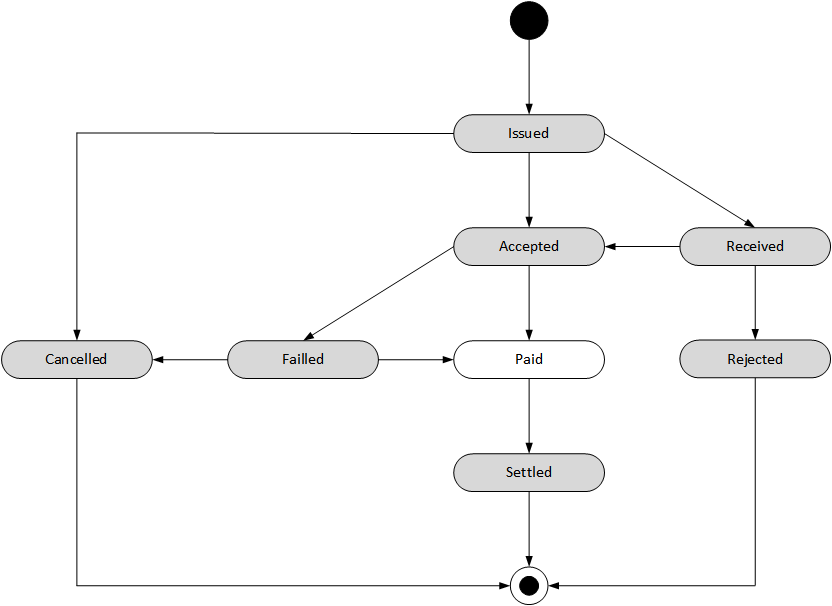
\includegraphics[width=9cm,angle=0]{./diag/Reference/DebitNoteState-Reference.png}
	\caption{Debit Note Status Diagram}
    \label{fig:DNSD}
\end{figure}

\begin{table}[H]
\footnotesize

\begin{center}
\begin{tabular}{|p{3cm}|p{11cm}|} 
\hline
\rowcolor{lightgray}	Status	& 	Description \\
\hline

Issued		&	 	\\
\hline
Received	&		\\
\hline
Accepted 	& 		\\
\hline
Rejected 	&		\\
\hline
Failed		&		\\
\hline
Settled		&		\\
\hline
Cancelled	&		\\
\hline
Paid		&	currently not implemented	\\
\hline

\end{tabular}
\end{center}
\end{table}

\end{enumerate}

\item Invoice

\begin{enumerate}

\item Object Description

The Invoice object is issued by the Provider node for the Requestor node,
in the context of a specific Agreement (Agreement object).
The context of the agreement is defined as a set of consents to the provision of a service and which was made within the Activity.
It indicates the total amount due from the Applicant under this Agreement.
After the Invoice is issued, no further Debit Notes will be issued.
Issuing an Invoice means Termination of the Agreement (if it has not already been terminated).
After the Invoice is issued, no Activities are allowed to be performed.


\item Object Fields

\begin{table}[H]
\footnotesize

\begin{center}
\begin{tabular}{|p{3cm}|l|p{3cm}|p{3cm}|p{4cm}|} 
\hline
\rowcolor{lightgray}	Name	& MO.	& Type	& Example & 	Description \\
\hline

invoiceId	 			& M & string 				&  							&  Debit Note Identifier \\
\hline	

timestamp 				& M & string(\$date-time) 	&  YYYY-MM-DDThh:mm:ss.sssZ	&  \\
\hline

agreementId				& M & string 				&  							&  Agreement Identifier \\
\hline	

activityIds				& O & string(list)			&							& List of activityIds \\
\hline

amount	 				& M & string 				&  							&   \\
\hline

issuerId				& M &  string				&							& Issuer Identifier \\
\hline

recipientId				& M & string 				&  							&   \\
\hline

payeeAddr				& M & string 				&  							&   \\
\hline

payerAddr				& M & string 				&  							&   \\
\hline

paymentPlatform			& M & object(json) 			&  							&   \\
\hline

paymentDueDate			& M & string(\$date-time) 	&  YYYY-MM-DDThh:mm:ss.sssZ	&  \\
\hline

status					& M & string(enum)			& [ ISSUED, RECEIVED, ACCEPTED, REJECTED, FAILED, SETTLED, CANCELLED ] & Invoice Status \\
\hline
			
\end{tabular}
\end{center}
\end{table}

\item Object State

(Please see Figure ~\ref{fig:ISD} on page ~\pageref{fig:ISD}).

\begin{figure}[H]
    \centering
    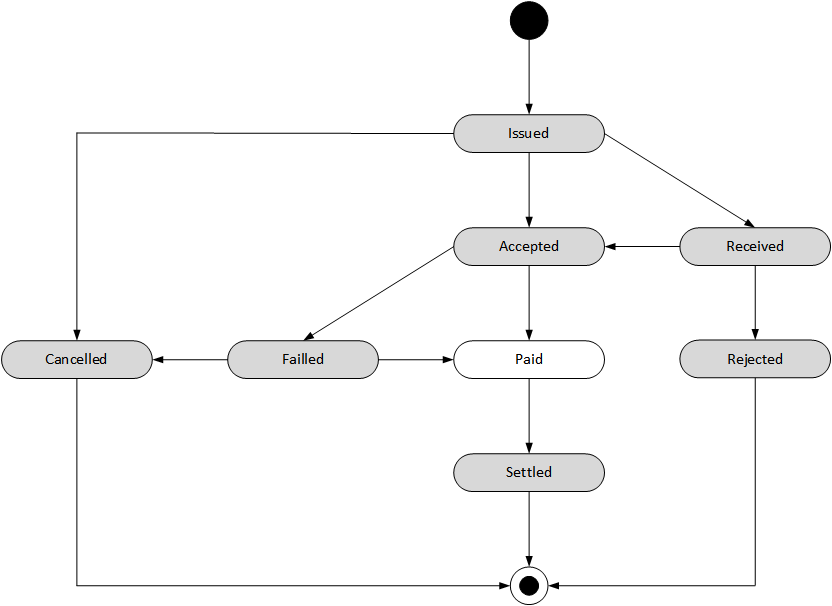
\includegraphics[width=9cm,angle=0]{./diag/Reference/InvoiceState-Reference.png}
	\caption{Invoice Status Diagram}
    \label{fig:ISD}
\end{figure}

\begin{table}[H]
\footnotesize

\begin{center}
\begin{tabular}{|p{3cm}|p{11cm}|} 
\hline
\rowcolor{lightgray}	Status	& 	Description \\
\hline

Issued		&	 	\\
\hline
Received	&		\\
\hline
Accepted 	& 		\\
\hline
Rejected 	&		\\
\hline
Failed		&		\\
\hline
Settled		&		\\
\hline
Cancelled	&		\\
\hline
Paid		&	currently not implemented	\\
\hline

\end{tabular}
\end{center}
\end{table}

\end{enumerate}


\item PaymentPlatform Object

\begin{enumerate}

\item Object Description

PaymentPlatform is a object that is helping to chose which driver and network to use

\item Object Fields

\begin{table}[H]
\footnotesize

\begin{center}
\begin{tabular}{|p{3cm}|l|p{3cm}|p{3cm}|p{4cm}|} 
\hline
\rowcolor{lightgray}	Name	& MO.	& Type	& Example & 	Description \\
\hline

driver		& O & string				&							& 							\\
\hline
network		& O & string				&							& 							\\
\hline
token		& O & string				&							& 							\\
\hline

\end{tabular}
\end{center}
\end{table}

\item Object State

Stateless object

\end{enumerate}

% Allocation

\item Allocation Object

\begin{enumerate}

\item Object Description

An Allocation is a designated sum of money reserved for the purpose of making some particular payments. 
Allocations are currently purely virtual objects. 
They exist only in Requestor's database. 
An Allocation is connected to a payment account (wallet) specified by address and paymentPlatform field. 
If these fields are not present the default payment platform is used and the address is assumed to be 
identical to the Requestor's Node ID.

\item Object Fields

\begin{table}[H]
\footnotesize

\begin{center}
\begin{tabular}{|p{3cm}|l|p{3cm}|p{3cm}|p{4cm}|} 
\hline
\rowcolor{lightgray}	Name	& MO.	& Type	& Example & 	Description \\
\hline

allocationId			& M & string 				&							&  \\
\hline

address					& O & string 				&							&  \\
\hline

paymentPlatform			& O & object(json)			&							&	\\
\hline

totalAmount				& M & string 				&							&  \\
\hline

spentAmount				& M & string 				&							&  \\
\hline

remainingAmount			& M & string 				&							&  \\
\hline

timestamp 				& M & string(\$date-time) 	&  YYYY-MM-DDThh:mm:ss.sssZ	&  \\
\hline

timeout					& O & string(\$date-time) ?? &							&  \\
\hline

makeDeposit				& O & boolean				&							&  \\
\hline

extendTimeout			& O & integer(\$int64)		&							& 	in seconds, the time by which the allocation timeout is extended 
																					after it is last used. \\
\hline

deposit.id				& M & string 				&							&  \\
\hline

deposit.contract		& M & string 				&							&  \\
\hline

deposit.validate		& O & json					& 							& 	\\
\hline
			
\end{tabular}
\end{center}
\end{table}

\item Object State

Stateless object

\end{enumerate}

\item AgreementPayment Object

\begin{enumerate}

\item Object Description

Share of a Payment assigned to an Agreement, but not to any particular Activity within that Agreement.

\item Object Fields

\begin{table}[H]
\footnotesize

\begin{center}
\begin{tabular}{|p{3cm}|l|p{3cm}|p{3cm}|p{4cm}|} 
\hline
\rowcolor{lightgray}	Name	& MO.	& Type	& Example & 	Description \\
\hline

agreementId		& M & string				&							& 							\\
\hline

amount			& M & string				&							& 							\\
\hline

allocationId	& O & string				&							& 							\\
\hline

\end{tabular}
\end{center}
\end{table}

\item Object State

Stateless object

\end{enumerate}

\item ActivityPayment Object

\begin{enumerate}

\item Object Description

Share of a Payment assigned to a particular Activity.

\item Object Fields

\begin{table}[H]
\footnotesize

\begin{center}
\begin{tabular}{|p{3cm}|l|p{3cm}|p{3cm}|p{4cm}|} 
\hline
\rowcolor{lightgray}	Name	& MO.	& Type	& Example & 	Description \\
\hline

activityId		& M & string				&							& 							\\
\hline

amount			& M & string				&							& 							\\
\hline

allocationId	& O & string				&							& 							\\
\hline

\end{tabular}
\end{center}
\end{table}

\item Object State

Stateless object

\end{enumerate}

\item Payment Object

\begin{enumerate}

\item Object Description

A Payment is a single transaction sent from Requestor to Provider. 
A single payment can be made for multiple Agreements and Activities. 
AgreementPayments and ActivityPayments specify what is the basis for payment.

\item Object Fields

\begin{table}[H]
\footnotesize

\begin{center}
\begin{tabular}{|p{3cm}|l|p{3cm}|p{3cm}|p{4cm}|} 
\hline
\rowcolor{lightgray}	Name	& MO.	& Type	& Example & 	Description \\
\hline

paymentId			& M & string				&							&							\\
\hline

payerId				& M & string				&							&							\\
\hline

payeeId				& M & string				&							&							\\
\hline

payerAddr			& M & string				&							&							\\
\hline

payeeAddr			& M & string				&							&							\\
\hline

paymentPlatform		& M & string				&							&							\\
\hline

amount				& M & string				&							&							\\
\hline

timestamp			& M & string(\$date-time)	&							&							\\
\hline

agreementPayments	& M & object(json)			&							&							\\
\hline

activityPayments	& M & object(json)			&							&							\\
\hline
	
details				& M & string(\$byte)		&							&							\\
\hline

\end{tabular}
\end{center}
\end{table}

\item Object State

Stateless object

\end{enumerate}

\end{enumerate}

%%%% Payment Operations TODO

The Payment Space is used to define interaction operations on these objects such as:

\begin{enumerate}

\item  Billing Operation

\begin{enumerate}

\item Description

TODO!!!

(Please see Figure ~\ref{fig:BO} on page ~\pageref{fig:BO}).

\item Sequence Diagram

\begin{figure}[H]
    \centering
%    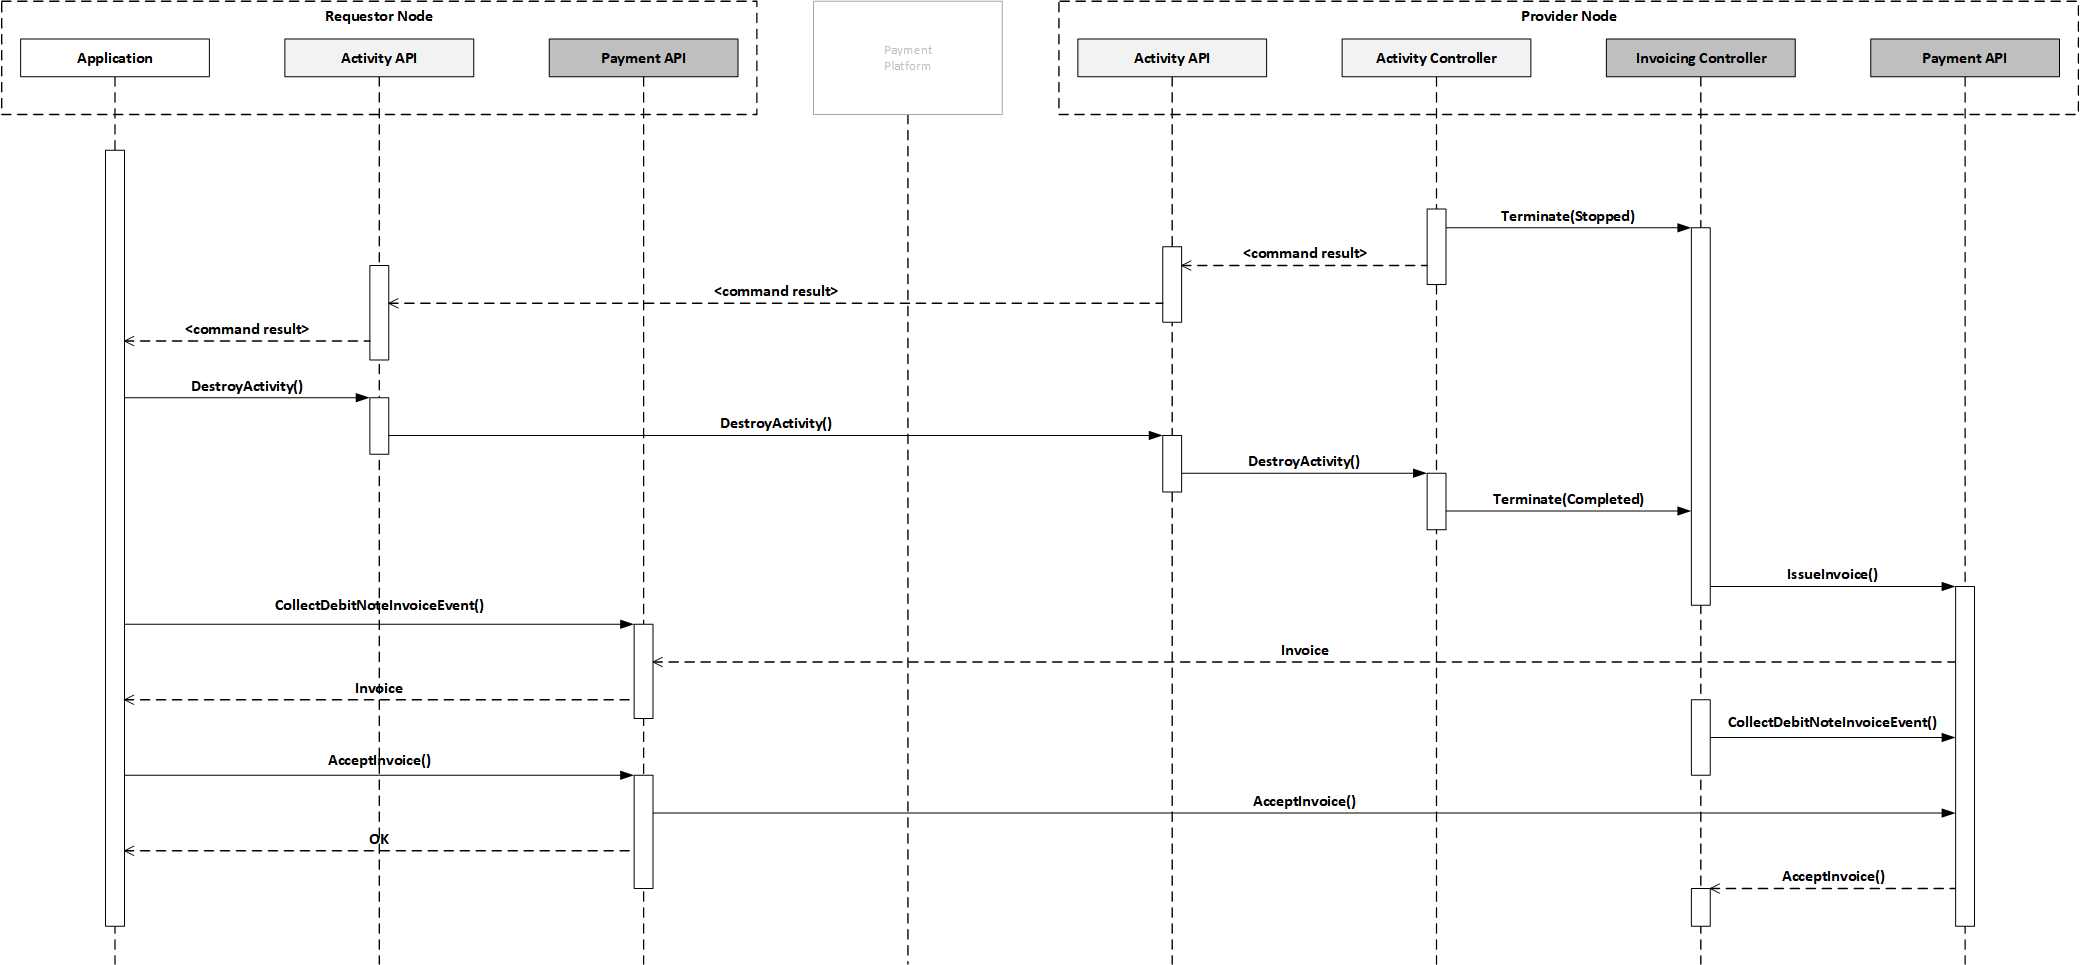
\includegraphics[width=14cm,angle=0]{./diag/Sequence/PaymentBilling-B-Sequence.png}
	\caption{Billing Operation}
    \label{fig:BO}
\end{figure}

\item Functions and Methods

\begin{table}[H]
\footnotesize

\begin{center}
\begin{tabular}{|p{3cm}|p{7cm}|p{1.5cm}|p{4cm}|} 
\hline
\rowcolor{lightgray}	Function Name	& API Method Name				& 	Side		&	Description \\
\hline

IssueDebitNote			&	POST /debitNotes							& 	Provider	&	Issue a Debit Note	\\
\hline

						& 	POST /debitNotes/\{debitNoteId\} /send		&	Provider 	&	Send Debit Note to Requestor \\
\hline

CancelDebitNote			&	POST /debitNotes/\{debitNoteId\} /cancel	&	Provider	&	Cancel Debit Note \\
\hline

CollectDebitNote \newline InvoiceEvent	&	GET /debitNoteEvents		&	Both		&	Get Debit Note events \\
\hline

AcceptDebitNote			&	POST /debitNotes/\{debitNoteId\} /accept	&	Requestor	&	Accept received Debit Note \\
\hline

						& 	GET /debitNotes								&	Both		& 	List Debit Notes \\
\hline

						& 	GET /debitNotes/\{debitNoteId\}				&	Both 		&	Get Debit Note \\
\hline

RejectDebitNote			&	POST /debitNotes/\{debitNoteId\} /reject	&	Requestor	&	Reject received Debit Note \\
\hline

IssueInvoice			&	POST /invoices								&	Provider	&	Issue an Invoice \\
\hline

AcceptInvoice			&	POST /invoices/\{invoiceId\} /accept		&	Requestor 	&	Accept received Invoice \\
\hline

RejectInvoice			&	POST /invoices/\{invoiceId\} /reject		&	Requestor 	&	Reject received Invoice \\
\hline

						& 	GET /invoices 								&	Both		&	List Invoices \\
\hline

						&	GET /invoices/\{invoiceId\}					&	Both		& 	Get Invoice \\
\hline

						&	POST /invoices/\{invoiceId\} /send			&	Provider 	& 	Send Invoice to Requestor \\
\hline 

						&	POST /invoices/\{invoiceId\} /cancel		&	Provider 	& 	Cancel Invoice  \\
\hline

						&	GET /invoiceEvents							&	Both 		& 	Get Invoice events \\
\hline

RejectionReasion		&												&	Requestor	&	{\it Unsolicited service} 
																							\newline 	{\it Bad Service}
																							\newline 	{\it Incorrect Amount} \\
\hline
						
\end{tabular}
\end{center}
\end{table}

\end{enumerate}

\break

%%%% PAYMENT

\item Payment Operation

\begin{enumerate}

\item Description

TODO !!!

(Please see Figure ~\ref{fig:PO} on page ~\pageref{fig:PO}).

\item Sequence Diagram

\begin{figure}[H]
    \centering
%    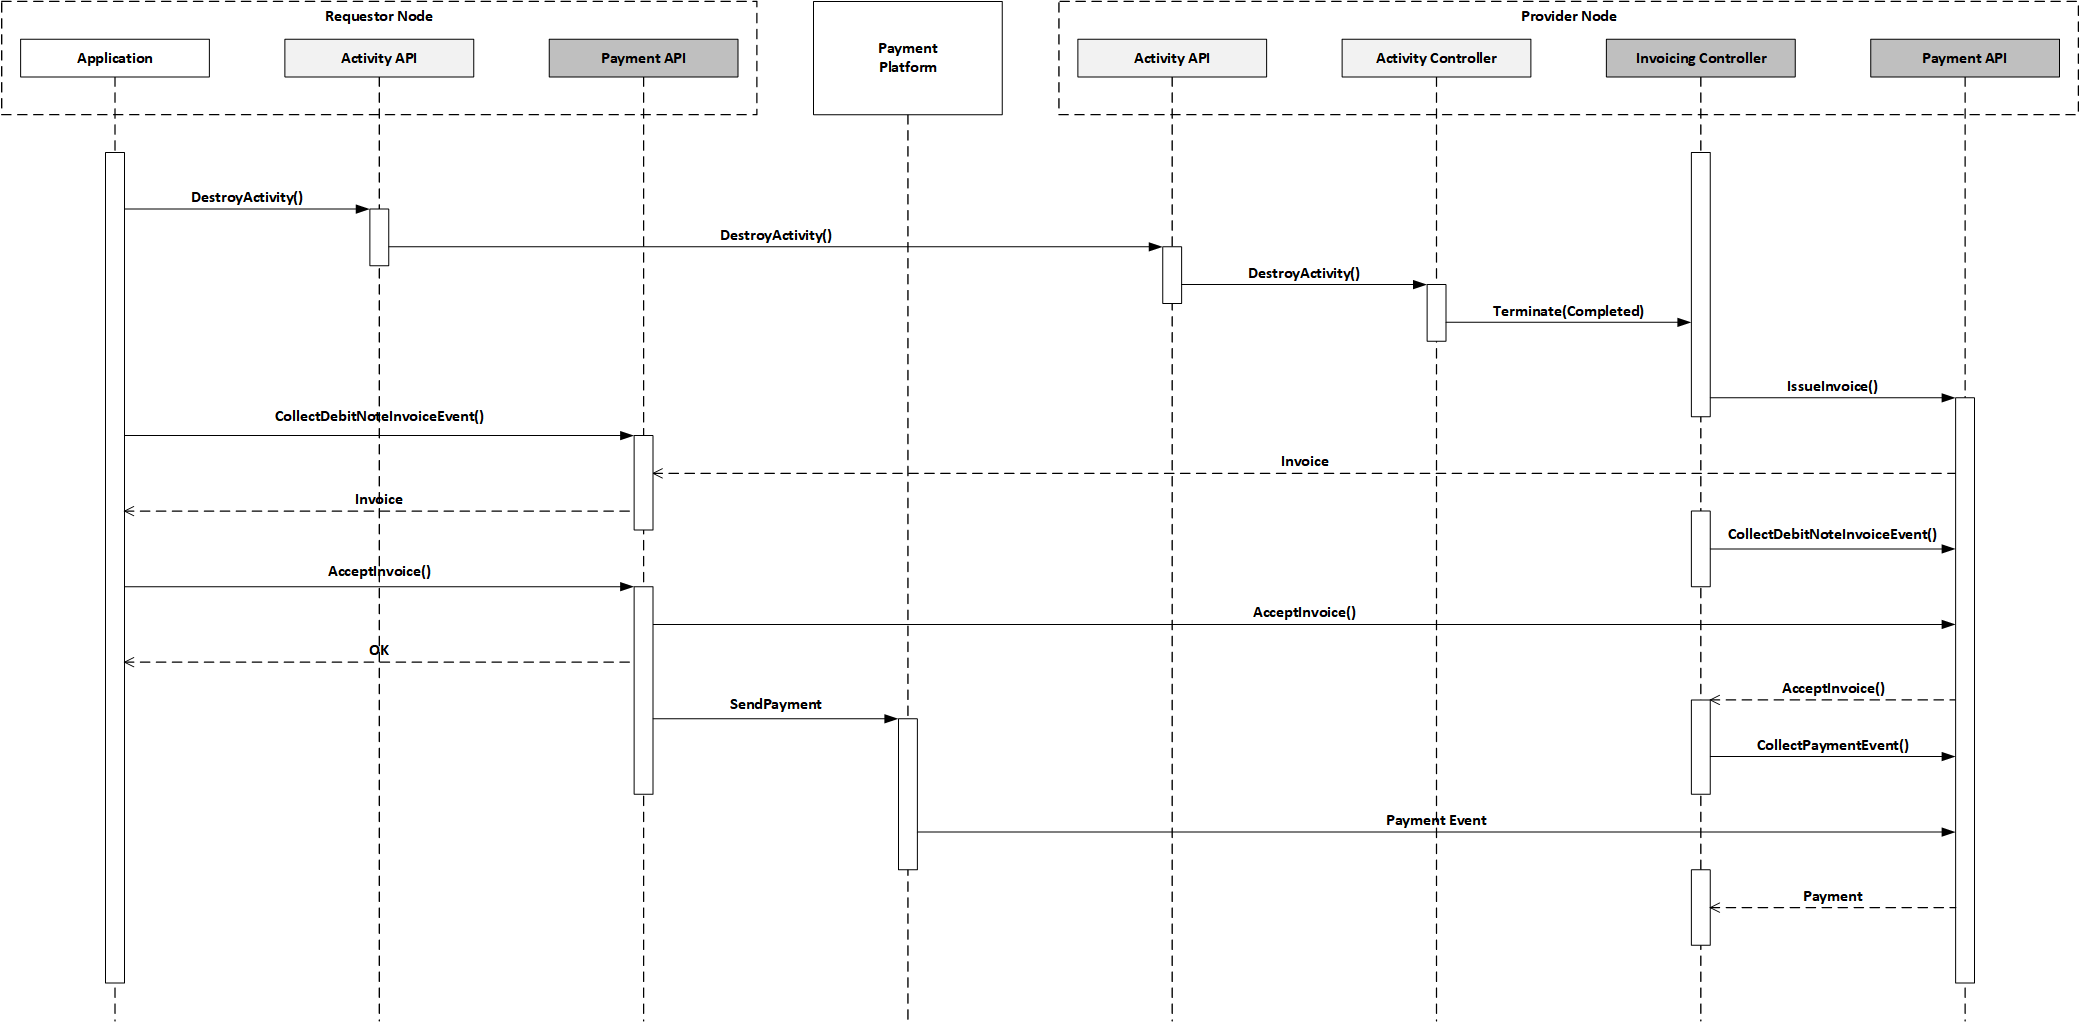
\includegraphics[width=14cm,angle=0]{./diag/Sequence/PaymentPayment-B-Sequence.png}
	\caption{Payment Operation}
    \label{fig:PO}
\end{figure}

\item Functions and Methods

\begin{table}[H]
\footnotesize

\begin{center}
\begin{tabular}{|p{3cm}|p{7cm}|p{1.5cm}|p{4cm}|} 
\hline
\rowcolor{lightgray}	Function Name	& API Method Name				& 	Side		&	Description \\
\hline

AllocateAmount			&	POST /allocations							&	Requestor 	&	Create Allocation \\
\hline

ListAllocations			&	GET /allocations 							&	Both		&	Get Allocations	\\
\hline

GetAllocationDetails	&	GET /allocations/\{allocationId\} 			&	Both		&	Get Allocation	\\
\hline

ReleaseAllocation		&	DELETE /allocations/\{allocationId\} 		&	Both		&	Release Allocation	\\
\hline

AmendAllocation			&	PUT /allocations/\{allocationId\} 			&	Both		&	Amend Allocation	\\
\hline

						&	GET /payments 								&	Both 		& 	Get payments \\
\hline

GetPaymentDetail		&	GET /payments/\{paymentId\}					&	Both 		&	Get payment \\
\hline

						& 	GET /payments/status 						& 	Both 		& 	Get status of the payment driver \\
\hline

CollectPaymentEvent		&												&	Provider 	&	Function used by Application process to 
																							collect notification of Payments arriving from PaymentPlatform \\
\hline

GetPayment ForDebitNote	&												&	Provider 	&	Function called by Provider to
																							obtain DebitNote-Payment mapping
																							required for payment reconciliation \\
\hline

GetPayment ForInvoice	&												&	Provider 	&	Function called by Provider to
																							obtain Invoice-Payment mapping
																							required for payment reconciliation \\
\hline

GetDemand Decorations	&	GET /demandDecorations 						&	Requestor	&	Function to extract the Demand (properties/constraints) specific to
																							a payment platform, which are necessary to place 
																							a payment-platform compliant Demand on the market \\
\hline

GetOffer Decorations	&						 						&	Provider	&	Function to extract the Offer (properties/constraints) specific to
																							a payment platform, which are necessary to place 
																							a payment-platform compliant Offer on the market \\
\hline
																									
						&	GET /providerAccounts						&	Provider 	&	Get available accounts for receiving payments \\
\hline

						&	GET /requestorAccounts						&	Requestor 	&	Get available accounts for receiving payments \\
\hline

GetSendAccounts			&												&	Requestor 	&	Function used by Application process on Requestor side to
																							list Accounts defined in the Daemon for the purpose of maiking payments. \\
\hline

GetReceiveAccounts		&												&	Provider 	&	Function used by Application process on Provider side to
																							list Accounts defined in the Daemon for the purpose of maiking payments. \\
\hline


\end{tabular}
\end{center}
\end{table}

\end{enumerate}

\end{enumerate}

%\begin{enumerate}
%    \item Service Profile
%    \item Service Protocol
%    \item Service Interface
%    \item Service Workflow
%\end{enumerate}

%\subsubsubsubsection{Registry and Discovery Service}

%\subsubsubsection{Golem Toolkit}

%\subsubsubsubsection{Golem Net Service API}

%\subsubsubsubsection{Golem Market Service API}

%\subsubsubsubsection{Golem Activity Service API}

%\subsubsubsubsection{Golem Payment Service API} 

%\subsubsubsubsection{Golem Rest Point}

%\subsubsection{Golem Central Net Server}



%\section{User Plane}
\section{User plane}

\subsection{Introduction}

\subsubsection{Ecosystem}

\subsubsubsection{SDK API}

\subsubsubsection{Examples}



%\section{External Provider Plane}
\section{External Provider Plane}

\subsection{Introduction}

\subsection{Payment Provider}

%\section{Layers}
\section{Layers}

\subsection{Platform Layer}

\subsection{Integration Layer}

\newpage

\subsubsection{Golem Toolkit}

\subsubsubsection{Introduction}

\subsubsubsection{Golem Market Service API}

\newpage

% MarketApiFunctions-FSAD-210

\subsubsubsubsection{SubscribeOffer Function}

\begin{enumerate}

\item Profile

\begin{enumerate}

\item Description

The SubscribeOffer function is used to publish the Provider Offer on the Golem Market. It uses the POST /offers method.
The Offer object is a set of properties and constraints of the sale item (e.g. computational resources like CPU, MEM, HDD, GPU, NIC)

\item Side

Provider

\end{enumerate}

\item Request

\begin{enumerate}

\item Input

\begin{tcolorbox}[boxrule=0pt, frame empty]
\begin{verbatim}

No parameters

\end{verbatim}
\end{tcolorbox}

Offer Object

\begin{tcolorbox}[boxrule=0pt, frame empty]
\begin{verbatim}

{
  "properties": {},
  "constraints": "string"
}

\end{verbatim}
\end{tcolorbox}

\begin{center}
\begin{tabular}{|p{3cm}|l|p{3cm}|p{3cm}|p{4cm}|} 
\hline
\rowcolor{lightgray}	Name	& MO.	& Type	& Example & 	Description \\
\hline

properties	& M	& 	json or flat	&		&	Offer properties \\ 

\hline

constraints	& O	& 	string	&		&	Offer constraints \\ 

\hline

\end{tabular}
\end{center}

\item REST Method

\begin{tcolorbox}[boxrule=0pt, frame empty]
\begin{verbatim} 

POST /offers

\end{verbatim}
\end{tcolorbox}

\end{enumerate}

\item Response

\begin{center}
\begin{tabular}{|c|l|} 
\hline
\rowcolor{lightgray}	Code 		& 	Description \\
\hline
201	 		&	Subscribed \\
\hline
400			&	(400) Bad request \\
\hline
401			&	(401) Authorization information is missing or invalid. \\
\hline
default		&	Unexpected error. \\
\hline
\end{tabular}
\end{center}


\item Result

\begin{tcolorbox}[boxrule=0pt, frame empty]
\begin{verbatim}

subscriptionId

\end{verbatim}
\end{tcolorbox}

\begin{center}
\begin{tabular}{|p{3cm}|l|p{3cm}|p{3cm}|p{4cm}|} 
\hline
\rowcolor{lightgray}	Name	& MO.	& Type	& Example & 	Description \\
\hline

subscriptionId	&	& 	string	&		&	Subscription Identifier \\ 

\hline

\end{tabular}
\end{center}


\item Workflow

(Please see Figure ~\ref{fig:SubsOffer} on page ~\pageref{fig:SubsOffer}):

\begin{figure}[htbp]
    \centering
    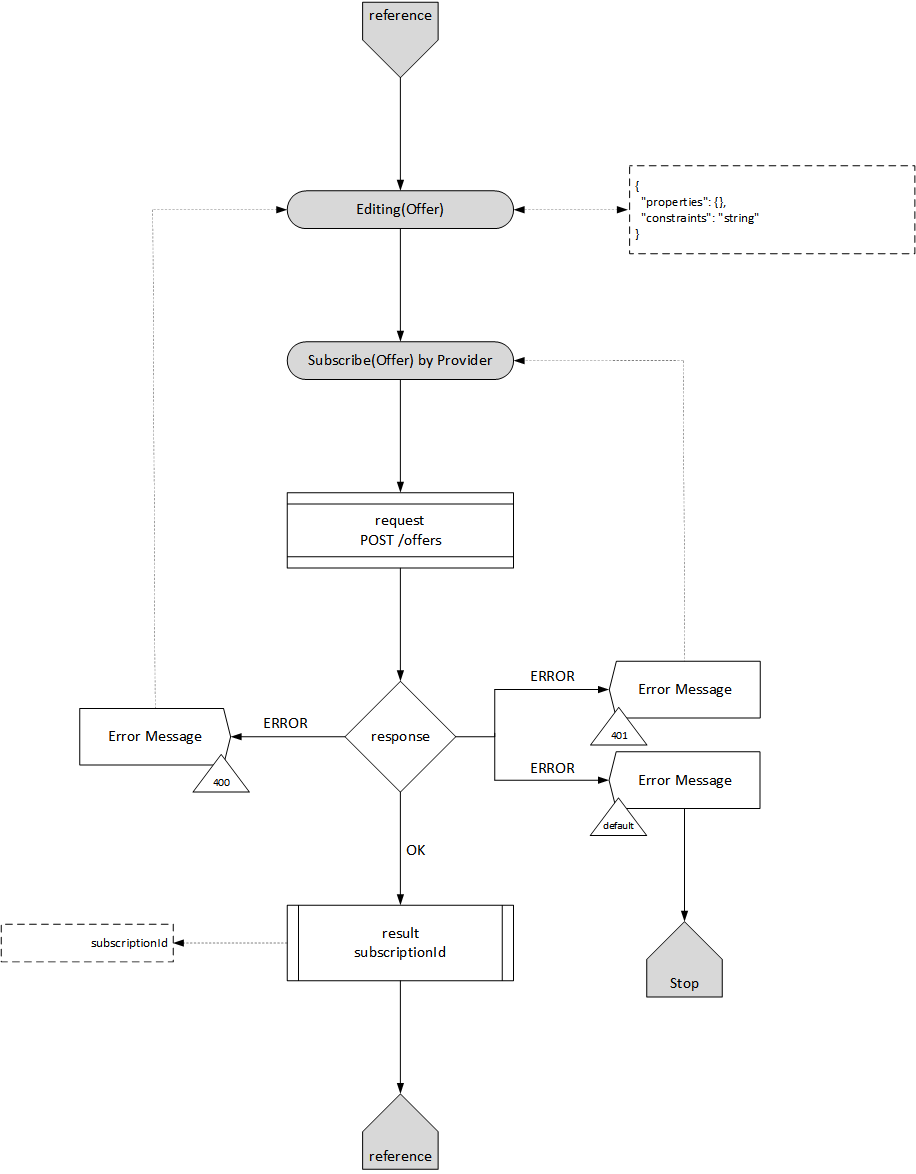
\includegraphics[width=12cm,height=12cm,angle=0]{./diag/Workflow/Market/SubscribeOffer-P-Workflow.png}
    \caption{Provider SubscribeOffer Workflow}
	\label{fig:SubsOffer}
\end{figure}


\end{enumerate}

\newpage

%% Unsubscribe Offer 
\subsubsubsubsection{UnsubscribeOffer Function}

\begin{enumerate}

\item Profile

\begin{enumerate}

\item Description

The UnsubscribeOffer function is used to stop receiving Demand Proposals for a Provider from Golem Market. 
It uses the DELETE /offers/\{subscriptionId\} method.

\item Side

Provider

\end{enumerate}

\item Request

\begin{enumerate}

\item Input

\begin{tcolorbox}[boxrule=0pt, frame empty]
\begin{verbatim}

subscriptionId

\end{verbatim}
\end{tcolorbox}

%Demand Object

%\begin{tcolorbox}[boxrule=0pt, frame empty]
%\begin{verbatim}

%{
%  "properties": {},
%  "constraints": "string"
%}

%\end{verbatim}
%\end{tcolorbox}

\begin{center}
\begin{tabular}{|p{3cm}|l|p{3cm}|p{3cm}|p{4cm}|} 
\hline
\rowcolor{lightgray}	Name	& MO.	& Type	& Example & 	Description \\
\hline

subscriptionId	& M	& 	string	&		&	Subscription Identifier \\ 

\hline

\end{tabular}
\end{center}

\item REST Method

\begin{tcolorbox}[boxrule=0pt, frame empty]
\begin{verbatim} 

DELETE /offers/{subscriptionId}

\end{verbatim}
\end{tcolorbox}

\end{enumerate}

\item Response

\begin{center}
\begin{tabular}{|c|l|} 
\hline
\rowcolor{lightgray}	Code 		& 	Description \\
\hline
204	 		&	Offer revoked \\
\hline
%400			&	(400) Bad request \\
%\hline
401			&	(401) Authorization information is missing or invalid. \\
\hline
410			&	Already unsubscribed. \\
\hline
default		&	Unexpected error. \\
\hline
\end{tabular}
\end{center}

\item Result

\begin{tcolorbox}[boxrule=0pt, frame empty]
\begin{verbatim}

None

\end{verbatim}
\end{tcolorbox}

%\begin{center}
%\begin{tabular}{|p{3cm}|l|p{3cm}|p{3cm}|p{4cm}|} 
%\hline
%\rowcolor{lightgray}	Name	& MO.	& Type	& Example & 	Description \\
%\hline

%subscriptionId	&	& 	string	&		&	Subscription Identifier \\ 

%\hline

%\end{tabular}
%\end{center}


\item Workflow

(Please see Figure ~\ref{fig:UsO} on page ~\pageref{fig:UsO}):

\begin{figure}[htbp]
    \centering
    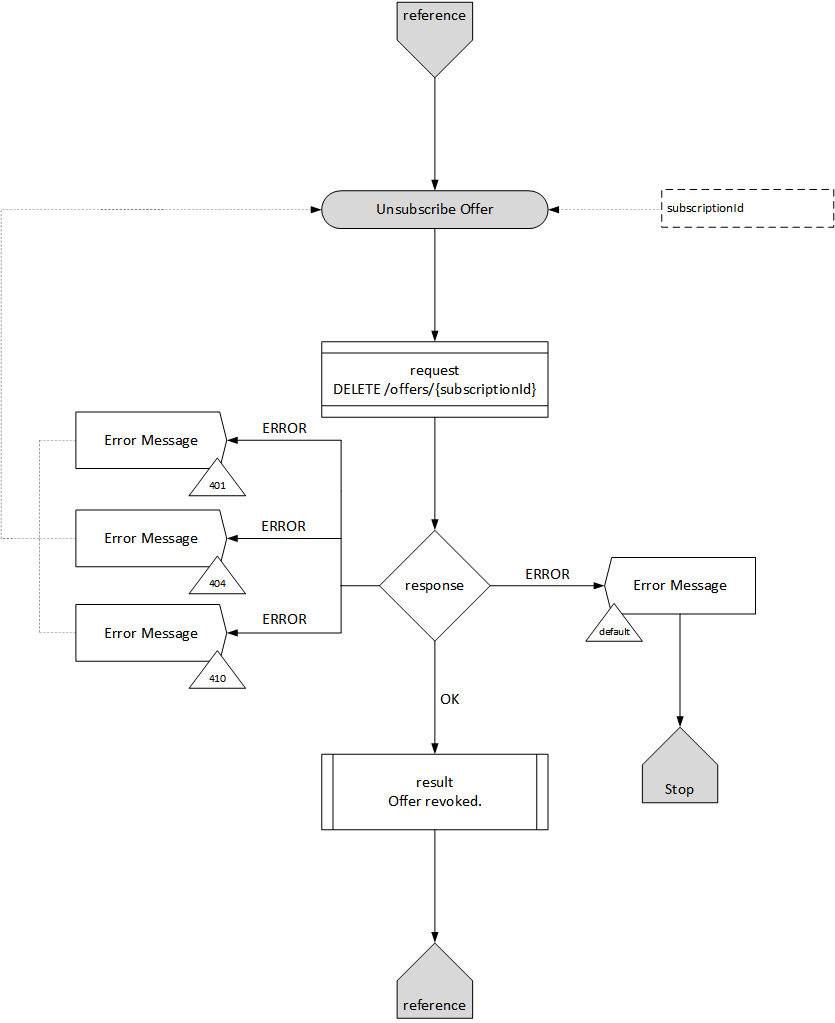
\includegraphics[width=12cm,height=12cm,angle=0]{./diag/Workflow/Market/UnsubscribeOffer-P-Workflow.png}
    \caption{Provider UnsubscribeOffer Workflow}
	\label{fig:UsO}
\end{figure}

\end{enumerate}

\newpage

\subsubsubsubsection{List(GetOffers) Function}

\begin{enumerate}

\item Profile

\begin{enumerate}

\item Description

The GetOffers function is used to fetch all active Offers which have been published by the Provider. 
It uses the GET /offers method.

\item Side

Provider

\end{enumerate}

\item Request

\begin{enumerate}

\item Input

\begin{tcolorbox}[boxrule=0pt, frame empty]
\begin{verbatim}

No parameters

\end{verbatim}
\end{tcolorbox}

%Offer Object

%\begin{tcolorbox}[boxrule=0pt, frame empty]
%\begin{verbatim}

%{
%  "properties": {},
%  "constraints": "string"
%}

%\end{verbatim}
%\end{tcolorbox}

%\begin{center}
%\begin{tabular}{|p{3cm}|l|p{3cm}|p{3cm}|p{4cm}|} 
%\hline
%\rowcolor{lightgray}	Name	& MO.	& Type	& Example & 	Description \\
%\hline

%properties	& M	& 	json or flat	&		&	Offer properties \\ 

%\hline

%constraints	& O	& 	string	&		&	Offer constraints \\ 

%\hline

%\end{tabular}
%\end{center}

\item REST Method

\begin{tcolorbox}[boxrule=0pt, frame empty]
\begin{verbatim} 

GET /offers

\end{verbatim}
\end{tcolorbox}

\end{enumerate}

\item Response

\begin{center}
\begin{tabular}{|c|l|} 
\hline
\rowcolor{lightgray}	Code 		& 	Description \\
\hline
200	 		&	Offer list. \\
\hline
400			&	(400) Bad request \\
\hline
401			&	(401) Authorization information is missing or invalid. \\
\hline
default		&	Unexpected error. \\
\hline
\end{tabular}
\end{center}


\item Result

\begin{tcolorbox}[boxrule=0pt, frame empty]
\begin{verbatim}

[
  {
    "properties": {},
    "constraints": "string",
    "offerId": "string",
    "providerId": "string",
    "timestamp": "YYYY-MM-DDThh:mm:ss.sssZ"
  }
]

\end{verbatim}
\end{tcolorbox}

\begin{center}
\begin{tabular}{|p{3cm}|l|p{3cm}|p{3cm}|p{4cm}|} 
\hline
\rowcolor{lightgray}	Name	& MO.	& Type	& Example & 	Description \\
\hline

properties	& 	& 	json or flat	&		&	Offer properties \\ 

\hline

constraints	& 	& 	string	&		&	Offer constraints \\ 

\hline

offerId		&	&	string	&		& 	Offer Identifier \\

\hline

providerId  & 	&	string	&		&	Provider's Node Identifier \\

\hline

timestamp	&	& 	string(\$date-time)	& YYYY-MM-DDThh:mm:ss.sssZ	&	Time of ???  \\ 

\hline

\end{tabular}
\end{center}


\item Workflow

(Please see Figure ~\ref{fig:LO} on page ~\pageref{fig:LO}):

\begin{figure}[htbp]
    \centering
    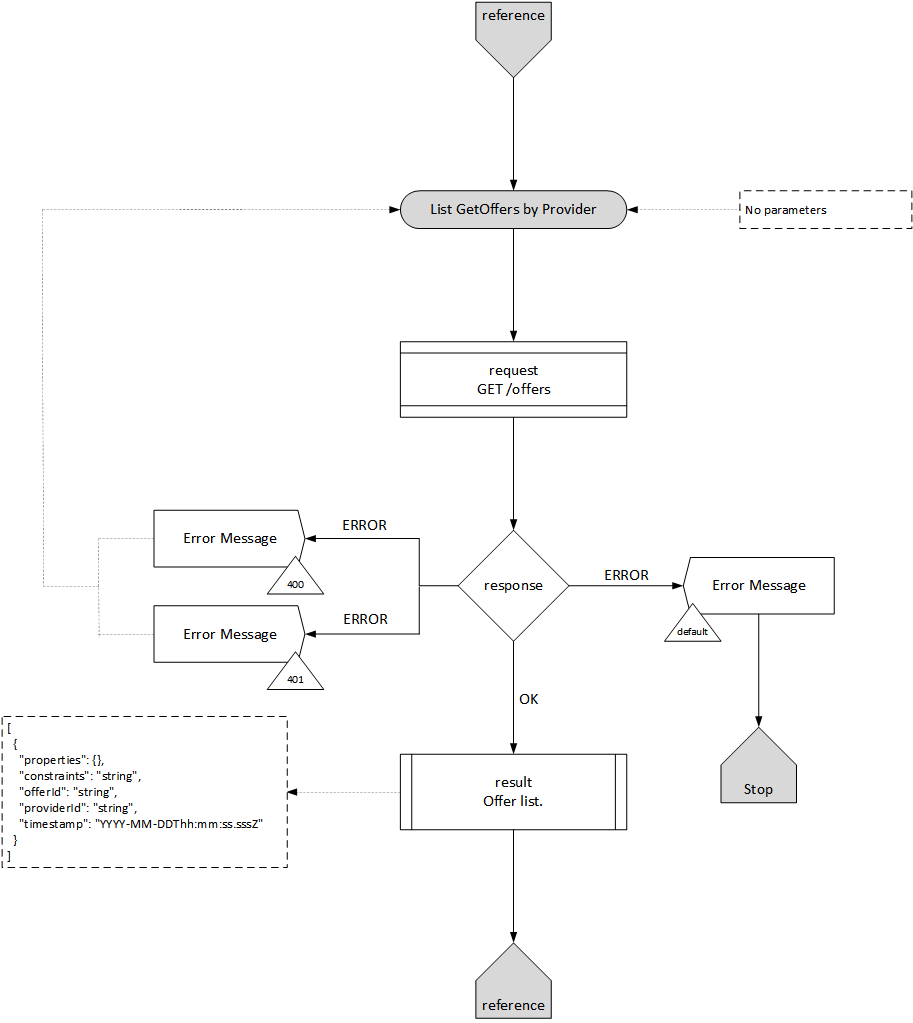
\includegraphics[width=12cm,height=12cm,angle=0]{./diag/Workflow/Market/List(GetOffers)-P-Workflow.png}
    \caption{Provider Workflow Active Offer List }
	\label{fig:LO}
\end{figure}


\end{enumerate}

\newpage

\subsubsubsubsection{CollectDemands Function}

\begin{enumerate}

\item Profile

\begin{enumerate}

\item Description

The CollectDemands function is used to read Market responses to published Offer by the Provider. 
It uses the GET /offers/\{subscriptionId\}/events method.

\item Side

Provider

\end{enumerate}

\item Request

\begin{enumerate}

\item Input

\begin{tcolorbox}[boxrule=0pt, frame empty]
\begin{verbatim}

subscriptionId
timeout
maxEvents

\end{verbatim}
\end{tcolorbox}

%Offer Object
%\begin{tcolorbox}[boxrule=0pt, frame empty]
%\begin{verbatim}
%{
%  "properties": {},
%  "constraints": "string"
%}
%\end{verbatim}
%\end{tcolorbox}

\begin{center}
\begin{tabular}{|p{3cm}|l|p{3cm}|p{3cm}|p{4cm}|} 
\hline
\rowcolor{lightgray}	Name	& MO.	& Type	& Example & 	Description \\
\hline

subscriptionId	& M	& 	string			&		&	Subscription Identifier \\ 

\hline

timeout			& O	& 	number(\$float)	&		&	Timeout used in long-polling calls (in seconds). 
													How many seconds server should wait for response containing new events 
													(0.0 means it should return immediately if there are no events).	Default value : 5 \\ 

\hline

maxEvents		& O & integer(\$int32)	&		&	Maximum number of events that server should return at once.		Default value : 10 \\

\hline	

\end{tabular}
\end{center}

\item REST Method

\begin{tcolorbox}[boxrule=0pt, frame empty]
\begin{verbatim} 

GET /offers/{subscriptionId}/events

\end{verbatim}
\end{tcolorbox}

\end{enumerate}

\item Response

\begin{center}
\begin{tabular}{|c|l|} 
\hline
\rowcolor{lightgray}	Code 		& 	Description \\
\hline
200	 		&	Proposal or Agreement event list. \\
\hline
404			&	(404) The specified resource was not found. \\
\hline
401			&	(401) Authorization information is missing or invalid. \\
\hline
default		&	Unexpected error. \\
\hline
\end{tabular}
\end{center}


\item Result

\begin{tcolorbox}[boxrule=0pt, frame empty]
\begin{verbatim}

[
  {
    "eventType": "string",
    "eventDate": "YYYY-MM-DDThh:mm:ss.sssZ"
  }
]

\end{verbatim}
\end{tcolorbox}

\begin{center}
\begin{tabular}{|p{3cm}|l|p{3cm}|p{3cm}|p{4cm}|} 
\hline
\rowcolor{lightgray}	Name	& MO.	& Type	& Example & 	Description \\
\hline

eventType	& 	& 	string	&		&	Event Type \\ 

\hline

eventDate	& 	& 	string(\$date-time)	&	YYYY-MM-DDThh:mm:ss.sssZ	&	Event Date \\ 

\hline

\end{tabular}
\end{center}


\item Workflow

(Please see Figure ~\ref{fig:CD} on page ~\pageref{fig:CD}):

\begin{figure}[htbp]
    \centering
    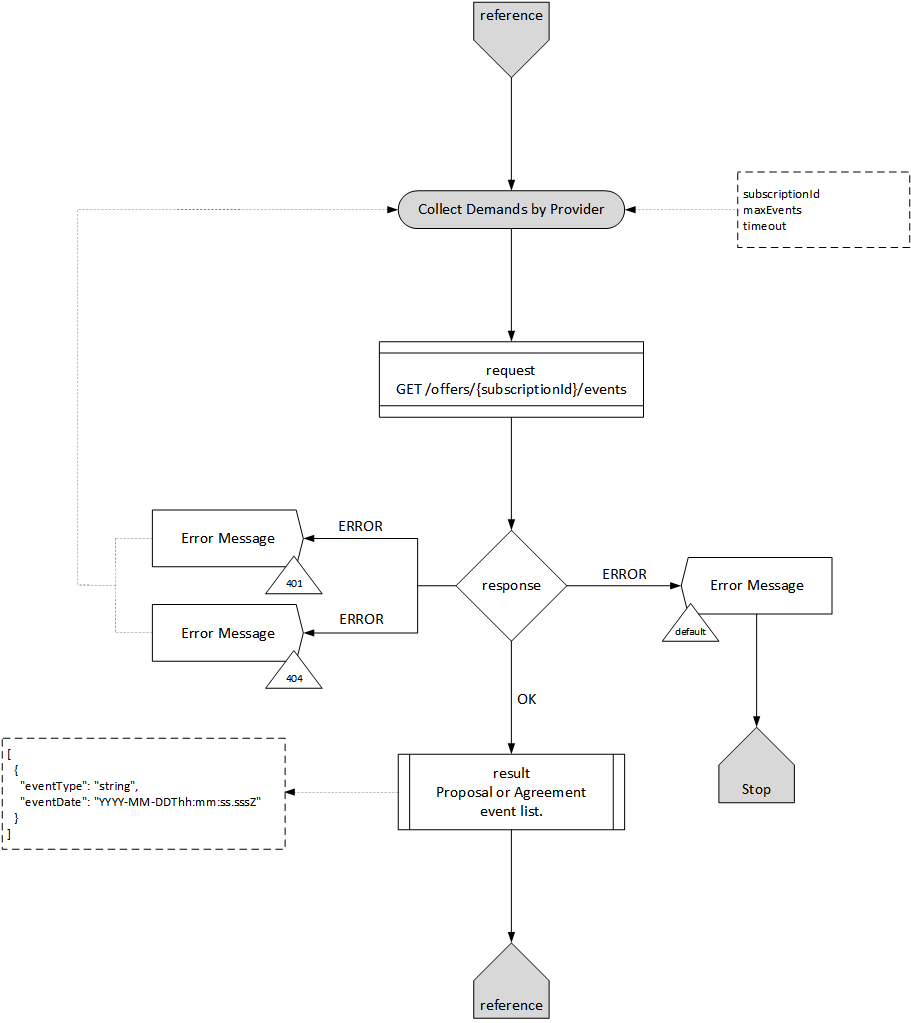
\includegraphics[width=11cm,height=11cm,angle=0]{./diag/Workflow/Market/CollectDemads-P-Workflow.png}
    \caption{Provider Workflow Collect Demands }
	\label{fig:CD}
\end{figure}


\end{enumerate}

\newpage

\subsubsubsubsection{GetProposalDemand Function}

\begin{enumerate}

\item Profile

\begin{enumerate}

\item Description

The GetProposalDemand function is used to fetch Proposal (Demand) with given id. 
It uses the GET /offers/\{subscriptionId\}/proposals/\{proposalId\} method.

\item Side

Provider

\end{enumerate}

\item Request

\begin{enumerate}

\item Input

\begin{tcolorbox}[boxrule=0pt, frame empty]
\begin{verbatim}

subscriptionId
proposalId

\end{verbatim}
\end{tcolorbox}

%Offer Object
%\begin{tcolorbox}[boxrule=0pt, frame empty]
%\begin{verbatim}
%{
%  "properties": {},
%  "constraints": "string"
%}
%\end{verbatim}
%\end{tcolorbox}

\begin{center}
\begin{tabular}{|p{3cm}|l|p{3cm}|p{3cm}|p{4cm}|} 
\hline
\rowcolor{lightgray}	Name	& MO.	& Type	& Example & 	Description \\
\hline

subscriptionId	& M	& 	string			&		&	Subscription Identifier \\ 

\hline

proposalId		& M & 	string			&		&	Proposal Identifier \\

\hline	

\end{tabular}
\end{center}

\item REST Method

\begin{tcolorbox}[boxrule=0pt, frame empty]
\begin{verbatim} 

GET /offers/{subscriptionId}/proposals/{proposalId}

\end{verbatim}
\end{tcolorbox}

\end{enumerate}

\item Response

\begin{center}
\begin{tabular}{|c|l|} 
\hline
\rowcolor{lightgray}	Code 		& 	Description \\
\hline
200	 		&	Proposal  \\
\hline
404			&	(404) The specified resource was not found. \\
\hline
401			&	(401) Authorization information is missing or invalid. \\
\hline
410			&	Proposal rejected. \\
\hline
default		&	Unexpected error. \\
\hline
\end{tabular}
\end{center}


\item Result

\begin{tcolorbox}[boxrule=0pt, frame empty]
\begin{verbatim}

{
  "properties": {},
  "constraints": "string",
  "proposalId": "string",
  "issuerId": "string",
  "state": "Initial",
  "timestamp": "YYYY-MM-DDThh:mm:ss.sssZ",
  "prevProposalId": "string"
}

\end{verbatim}
\end{tcolorbox}

\begin{center}
\begin{tabular}{|p{3cm}|l|p{3cm}|p{3cm}|p{4cm}|} 
\hline
\rowcolor{lightgray}	Name	& MO.	& Type	& Example & 	Description \\
\hline

properties	& 	& 	json or flat		&								&	 \\ 

\hline

constraints &	&	string				&								&	\\

\hline

proposalId	&	&	string				&								& Proposal Identifier \\

\hline

issuerId	&	&	string				&								& Issuer Node Id \\

\hline

state		&	&	enum				& [Initial, Draft, Rejected, Accepted, Expired] & Proposal State \\

\hline

timestamp	& 	& 	string(\$date-time)	&	YYYY-MM-DDThh:mm:ss.sssZ	&	Time ? \\ 

\hline

prevProposalId & &	string 				&								&	Id of the proposal from other side which this proposal responds to \\

\hline

\end{tabular}
\end{center}


\item Workflow

(Please see Figure ~\ref{fig:GPD} on page ~\pageref{fig:GPD}):

\begin{figure}[htbp]
    \centering
    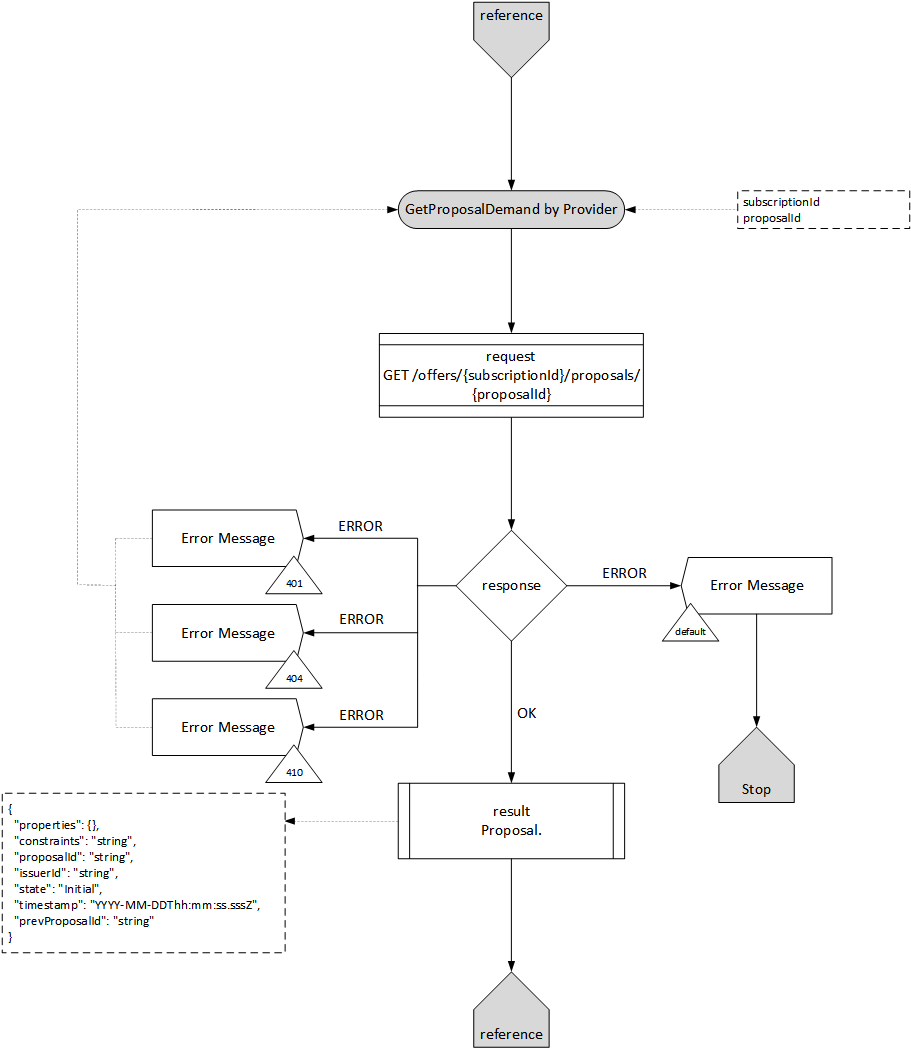
\includegraphics[width=12cm,height=12cm,angle=0]{./diag/Workflow/Market/GetProposalDemand-P-Workflow.png}
    \caption{Provider Workflow Get Proposal Demand }
	\label{fig:GPD}
\end{figure}


\end{enumerate}

\newpage

\subsubsubsubsection{CounterProposalOffer Function}

\begin{enumerate}

\item Profile

\begin{enumerate}

\item Description

The CounterProposalOffer function is used to respond with bespoke Offer to received Demand. 
It uses the POST /offers/\{subscriptionId\}/proposals/\{proposalId\} method.

\item Side

Provider

\end{enumerate}

\item Request

\begin{enumerate}

\item Input

\begin{tcolorbox}[boxrule=0pt, frame empty]
\begin{verbatim}

subscriptionId
proposalId

\end{verbatim}
\end{tcolorbox}

Offer Object
\begin{tcolorbox}[boxrule=0pt, frame empty]
\begin{verbatim}
{
  "properties": {},
  "constraints": "string"
}
\end{verbatim}
\end{tcolorbox}

\begin{center}
\begin{tabular}{|p{3cm}|l|p{3cm}|p{3cm}|p{4cm}|} 
\hline
\rowcolor{lightgray}	Name	& MO.	& Type	& Example & 	Description \\
\hline

subscriptionId	& M	& 	string			&		&	Subscription Identifier \\ 

\hline

proposalId		& M & 	string			&		&	Proposal Identifier \\

\hline	

properties		& M &	json or flat 	&		& Offer Properties		\\

\hline

constraints 	& M &	string			&		& Offer Constraints		\\

\hline

\end{tabular}
\end{center}

\item REST Method

\begin{tcolorbox}[boxrule=0pt, frame empty]
\begin{verbatim} 

POST /offers/{subscriptionId}/proposals/{proposalId}

\end{verbatim}
\end{tcolorbox}

\end{enumerate}

\item Response

\begin{center}
\begin{tabular}{|c|l|} 
\hline
\rowcolor{lightgray}	Code 		& 	Description \\
\hline
201	 		&	Counter Proposal created.  \\
\hline
400			&	(400) Bad request	\\
\hline
404			&	(404) The specified resource was not found. \\
\hline
401			&	(401) Authorization information is missing or invalid. \\
\hline
410			&	Proposal rejected. \\
\hline
default		&	Unexpected error. \\
\hline
\end{tabular}
\end{center}


\item Result

\begin{tcolorbox}[boxrule=0pt, frame empty]
\begin{verbatim}
  proposalId
\end{verbatim}
\end{tcolorbox}

\begin{center}
\begin{tabular}{|p{3cm}|l|p{3cm}|p{3cm}|p{4cm}|} 
\hline
\rowcolor{lightgray}	Name	& MO.	& Type	& Example & 	Description \\
\hline

proposalId	&	&	string				&								& Proposal Identifier \\

\hline

\end{tabular}
\end{center}


\item Workflow

(Please see Figure ~\ref{fig:CPO} on page ~\pageref{fig:CPO}):

\begin{figure}[htbp]
    \centering
    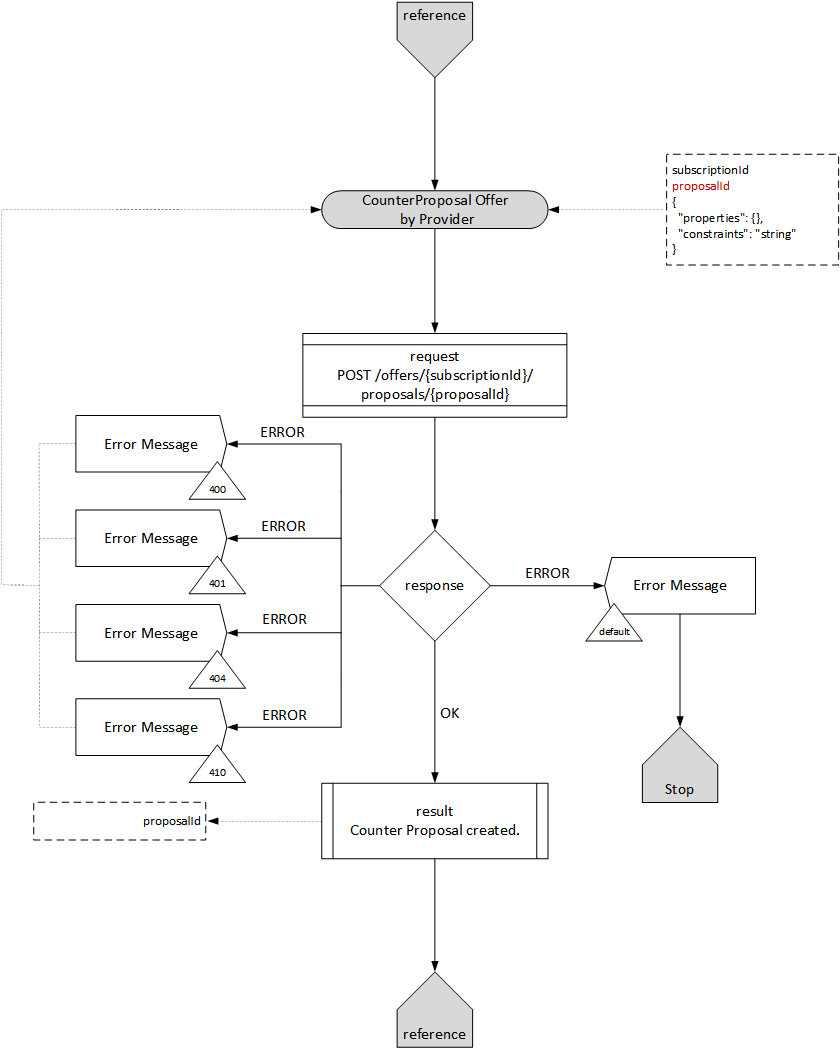
\includegraphics[width=12cm,height=12cm,angle=0]{./diag/Workflow/Market/CounterProposalOffer-P-Workflow.png}
    \caption{Provider Workflow Counter Proposal Offer }
	\label{fig:CPO}
\end{figure}


\end{enumerate}

\newpage

\subsubsubsubsection{RejectProposalDemand Function}

\begin{enumerate}

\item Profile

\begin{enumerate}

\item Description

The RejectProposalDemand function is used to reject Proposal Demand. \\
It uses the POST /offers/\{subscriptionId\}/proposals/\{proposalId\}/reject method.

\item Side

Provider

\end{enumerate}

\item Request

\begin{enumerate}

\item Input

\begin{tcolorbox}[boxrule=0pt, frame empty]
\begin{verbatim}

subscriptionId
proposalId

\end{verbatim}
\end{tcolorbox}

Object
\begin{tcolorbox}[boxrule=0pt, frame empty]
\begin{verbatim}
{
  "message": "string",
  "additionalProp1": {}
}
\end{verbatim}
\end{tcolorbox}

\begin{center}
\begin{tabular}{|p{3cm}|l|p{3cm}|p{3cm}|p{4cm}|} 
\hline
\rowcolor{lightgray}	Name	& MO.	& Type	& Example & 	Description \\
\hline

subscriptionId		& M	& 	string			&		&	Subscription Identifier \\ 

\hline

proposalId			& M & 	string			&		&	Proposal Identifier \\

\hline	

message				& O &	string 			&		& 		\\

\hline

additionalProp1 	& O &	json			&		& 		\\

\hline

\end{tabular}
\end{center}

\item REST Method

\begin{tcolorbox}[boxrule=0pt, frame empty]
\begin{verbatim} 

POST /offers/{subscriptionId}/proposals/{proposalId}/reject

\end{verbatim}
\end{tcolorbox}

\end{enumerate}

\item Response

\begin{center}
\begin{tabular}{|c|l|} 
\hline
\rowcolor{lightgray}	Code 		& 	Description \\
\hline
204	 		&	Proposal rejected.  \\
\hline
404			&	(404) The specified resource was not found. \\
\hline
401			&	(401) Authorization information is missing or invalid. \\
\hline
410			&	Proposal rejected. \\
\hline
default		&	Unexpected error. \\
\hline
\end{tabular}
\end{center}


\item Result

\begin{tcolorbox}[boxrule=0pt, frame empty]
\begin{verbatim}
  None
\end{verbatim}
\end{tcolorbox}

\item Workflow

(Please see Figure ~\ref{fig:RPD} on page ~\pageref{fig:RPD}):

\begin{figure}[htbp]
    \centering
    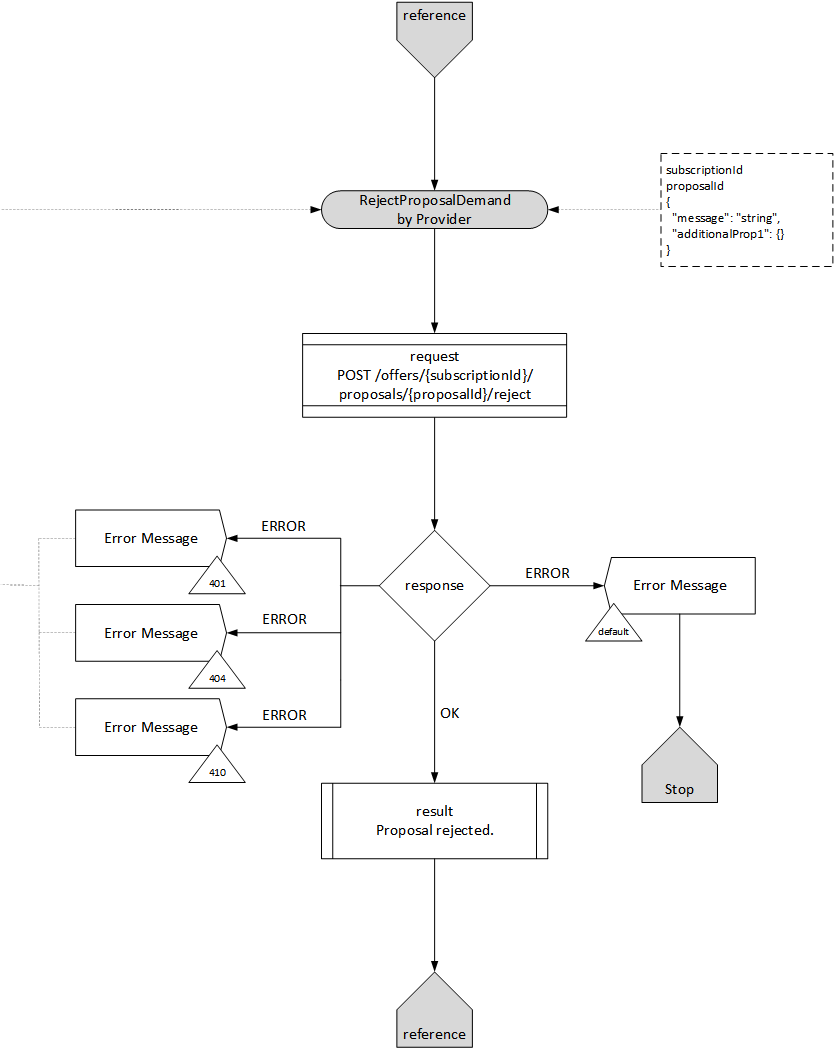
\includegraphics[width=12cm,height=12cm,angle=0]{./diag/Workflow/Market/RejectProposalDemand-P-Workflow.png}
    \caption{Provider Workflow Reject Proposal Demand }
	\label{fig:RPD}
\end{figure}


\end{enumerate}

\newpage


%%%%%%%%% Demand %%%%%%%%%%%%%%%%%%%%%%%%%%%%%

\subsubsubsubsection{SubscribeDemand Function}

\begin{enumerate}

\item Profile

\begin{enumerate}

\item Description

The SubscribeDemand function is used to publish the Requestor Demand on the Golem Market. It uses the POST /demands method.
The Demand object is a set of properties and constraints of the item being ordered (e.g., computing resources such as CPU, MEM, HDD, GPU, NIC)

\item Side

Requestor

\end{enumerate}

\item Request

\begin{enumerate}

\item Input

\begin{tcolorbox}[boxrule=0pt, frame empty]
\begin{verbatim}

No parameters

\end{verbatim}
\end{tcolorbox}

Demand Object

\begin{tcolorbox}[boxrule=0pt, frame empty]
\begin{verbatim}

{
  "properties": {},
  "constraints": "string"
}

\end{verbatim}
\end{tcolorbox}

\begin{center}
\begin{tabular}{|p{3cm}|l|p{3cm}|p{3cm}|p{4cm}|} 
\hline
\rowcolor{lightgray}	Name	& MO.	& Type	& Example & 	Description \\
\hline

properties	& M	& 	json or flat	&		&	Offer properties \\ 

\hline

constraints	& O	& 	string	&		&	Offer constraints \\ 

\hline

\end{tabular}
\end{center}

\item REST Method

\begin{tcolorbox}[boxrule=0pt, frame empty]
\begin{verbatim} 

POST /demands

\end{verbatim}
\end{tcolorbox}

\end{enumerate}

\item Response

\begin{center}
\begin{tabular}{|c|l|} 
\hline
\rowcolor{lightgray}	Code 		& 	Description \\
\hline
201	 		&	Subscribed \\
\hline
400			&	(400) Bad request \\
\hline
401			&	(401) Authorization information is missing or invalid. \\
\hline
default		&	Unexpected error. \\
\hline
\end{tabular}
\end{center}


\item Result

\begin{tcolorbox}[boxrule=0pt, frame empty]
\begin{verbatim}

subscriptionId

\end{verbatim}
\end{tcolorbox}

\begin{center}
\begin{tabular}{|p{3cm}|l|p{3cm}|p{3cm}|p{4cm}|} 
\hline
\rowcolor{lightgray}	Name	& MO.	& Type	& Example & 	Description \\
\hline

subscriptionId	&	& 	string	&		&	Subscription Identifier \\ 

\hline

\end{tabular}
\end{center}


\item Workflow

(Please see Figure ~\ref{fig:SubsDemand} on page ~\pageref{fig:SubsDemand}):

\begin{figure}[htbp]
    \centering
    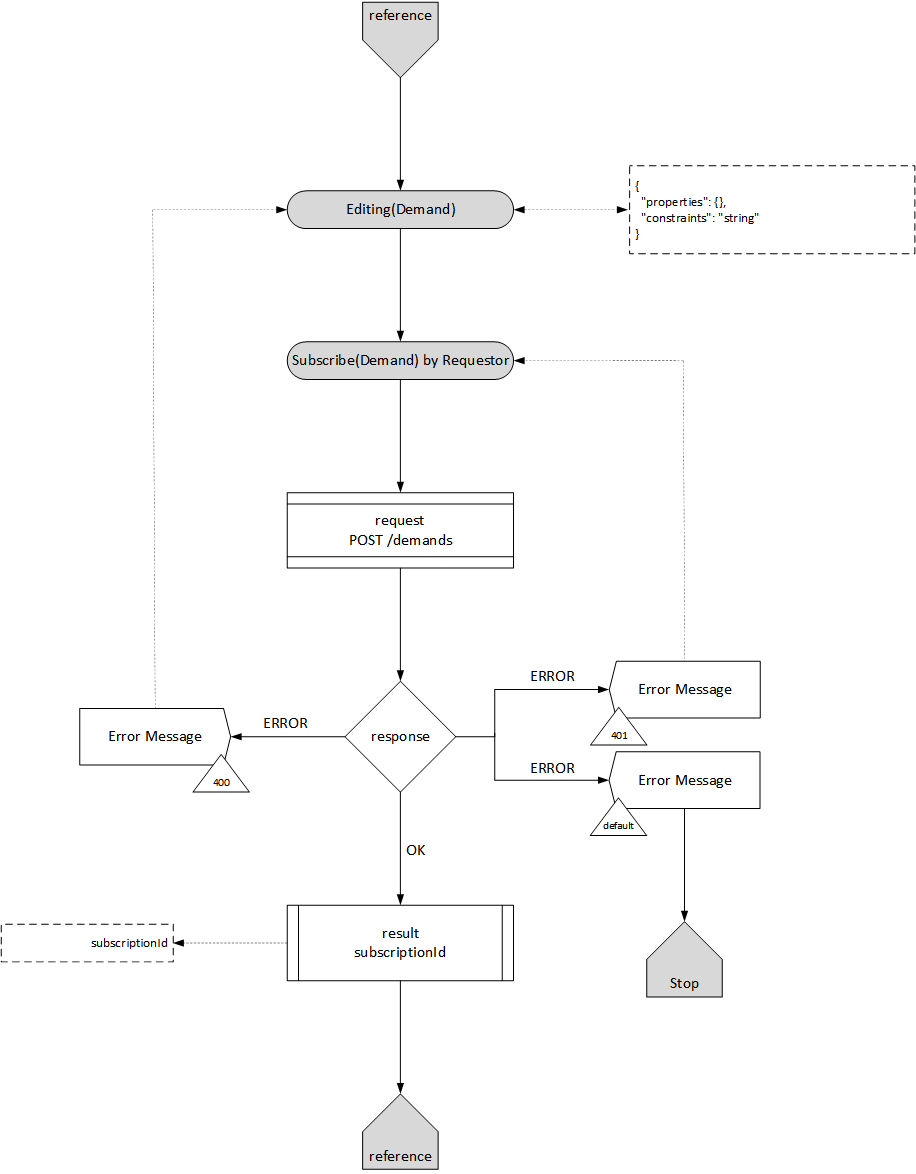
\includegraphics[width=12cm,height=12cm,angle=0]{./diag/Workflow/Market/SubscribeDemand-R-Workflow.png}
    \caption{Requestor SubscribeDemand Workflow}
	\label{fig:SubsDemand}
\end{figure}


\end{enumerate}

\newpage

%% Unsubscribe Demand 
\subsubsubsubsection{UnsubscribeDemand Function}

\begin{enumerate}

\item Profile

\begin{enumerate}

\item Description

The UnsubscribeDemand function is used to stop receiving Offer Proposals for a Requestor from Golem Market. \\ 
It uses the DELETE /demands/\{subscriptionId\} method.

\item Side

Requestor

\end{enumerate}

\item Request

\begin{enumerate}

\item Input

\begin{tcolorbox}[boxrule=0pt, frame empty]
\begin{verbatim}

subscriptionId

\end{verbatim}
\end{tcolorbox}

%Demand Object

%\begin{tcolorbox}[boxrule=0pt, frame empty]
%\begin{verbatim}

%{
%  "properties": {},
%  "constraints": "string"
%}

%\end{verbatim}
%\end{tcolorbox}

\begin{center}
\begin{tabular}{|p{3cm}|l|p{3cm}|p{3cm}|p{4cm}|} 
\hline
\rowcolor{lightgray}	Name	& MO.	& Type	& Example & 	Description \\
\hline

subscriptionId	& M	& 	string	&		&	Subscription Identifier \\ 

\hline

\end{tabular}
\end{center}

\item REST Method

\begin{tcolorbox}[boxrule=0pt, frame empty]
\begin{verbatim} 

DELETE /demands/{subscriptionId}

\end{verbatim}
\end{tcolorbox}

\end{enumerate}

\item Response

\begin{center}
\begin{tabular}{|c|l|} 
\hline
\rowcolor{lightgray}	Code 		& 	Description \\
\hline
204	 		&	Demand revoked \\
\hline
%400			&	(400) Bad request \\
%\hline
401			&	(401) Authorization information is missing or invalid. \\
\hline
410			&	Already unsubscribed. \\
\hline
default		&	Unexpected error. \\
\hline
\end{tabular}
\end{center}

\item Result

\begin{tcolorbox}[boxrule=0pt, frame empty]
\begin{verbatim}

None

\end{verbatim}
\end{tcolorbox}

%\begin{center}
%\begin{tabular}{|p{3cm}|l|p{3cm}|p{3cm}|p{4cm}|} 
%\hline
%\rowcolor{lightgray}	Name	& MO.	& Type	& Example & 	Description \\
%\hline

%subscriptionId	&	& 	string	&		&	Subscription Identifier \\ 

%\hline

%\end{tabular}
%\end{center}


\item Workflow

(Please see Figure ~\ref{fig:UsD} on page ~\pageref{fig:UsD}):

\begin{figure}[htbp]
    \centering
    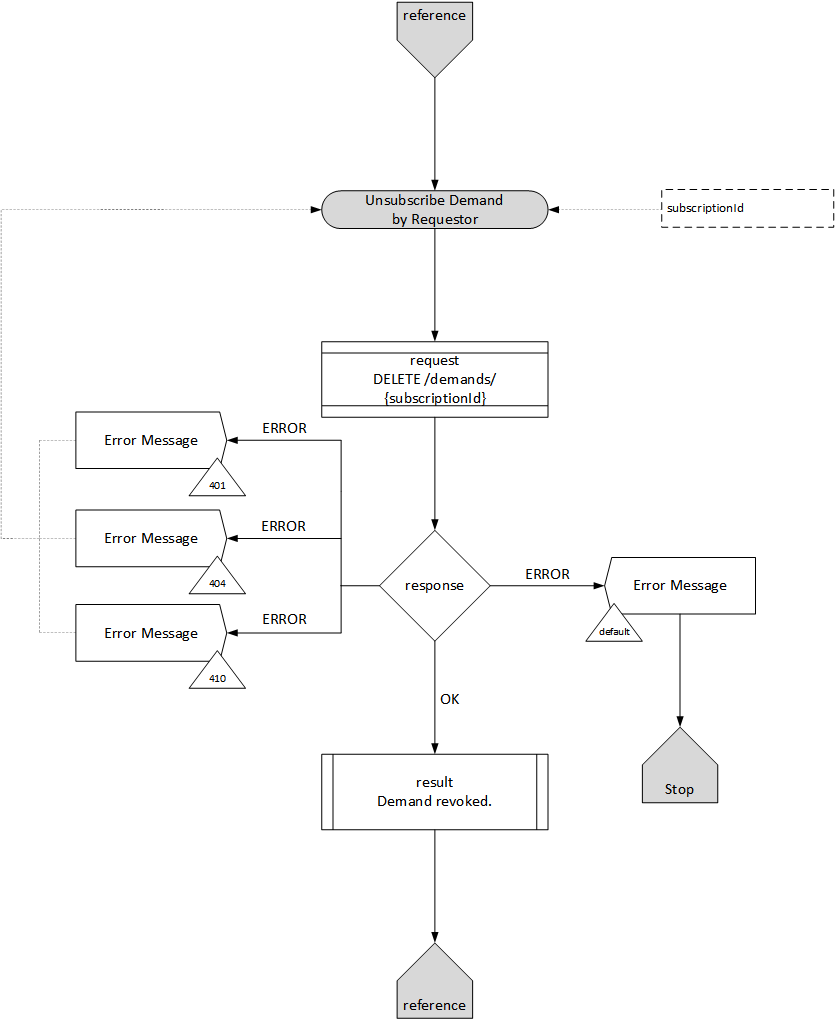
\includegraphics[width=12cm,height=12cm,angle=0]{./diag/Workflow/Market/UnsubsribeDemand-R-Workflow.png}
    \caption{Requestor UnsubscribeDemand Workflow}
	\label{fig:UsD}
\end{figure}

\end{enumerate}

\newpage

\subsubsubsubsection{List(GetDemands) Function}

\begin{enumerate}

\item Profile

\begin{enumerate}

\item Description

The GetDemands function is used to fetch all active Demands which have been published by the Requestor. \\ 
It uses the GET /offers method.

\item Side

Requestor

\end{enumerate}

\item Request

\begin{enumerate}

\item Input

\begin{tcolorbox}[boxrule=0pt, frame empty]
\begin{verbatim}

No parameters

\end{verbatim}
\end{tcolorbox}

\item REST Method

\begin{tcolorbox}[boxrule=0pt, frame empty]
\begin{verbatim} 

GET /offers

\end{verbatim}
\end{tcolorbox}

\end{enumerate}

\item Response

\begin{center}
\begin{tabular}{|c|l|} 
\hline
\rowcolor{lightgray}	Code 		& 	Description \\
\hline
200	 		&	Demand list. \\
\hline
400			&	(400) Bad request \\
\hline
401			&	(401) Authorization information is missing or invalid. \\
\hline
default		&	Unexpected error. \\
\hline
\end{tabular}
\end{center}


\item Result

\begin{tcolorbox}[boxrule=0pt, frame empty]
\begin{verbatim}

[
  {
    "properties": {},
    "constraints": "string",
    "demandId": "string",
    "requestorId": "string",
    "timestamp": "YYYY-MM-DDThh:mm:ss.sssZ"
  }
]

\end{verbatim}
\end{tcolorbox}

\begin{center}
\begin{tabular}{|p{3cm}|l|p{3cm}|p{3cm}|p{4cm}|} 
\hline
\rowcolor{lightgray}	Name	& MO.	& Type	& Example & 	Description \\
\hline

properties	& 	& 	json or flat	&		&	Demand properties \\ 

\hline

constraints	& 	& 	string	&		&	Demand constraints \\ 

\hline

demandId		&	&	string	&		& 	Demand Identifier \\

\hline

requestorId  & 	&	string	&		&	Requestor's Node Identifier \\

\hline

timestamp	&	& 	string(\$date-time)	& YYYY-MM-DDThh:mm:ss.sssZ	&	Time of ???  \\ 

\hline

\end{tabular}
\end{center}


\item Workflow

(Please see Figure ~\ref{fig:LD} on page ~\pageref{fig:LD}):

\begin{figure}[htbp]
    \centering
    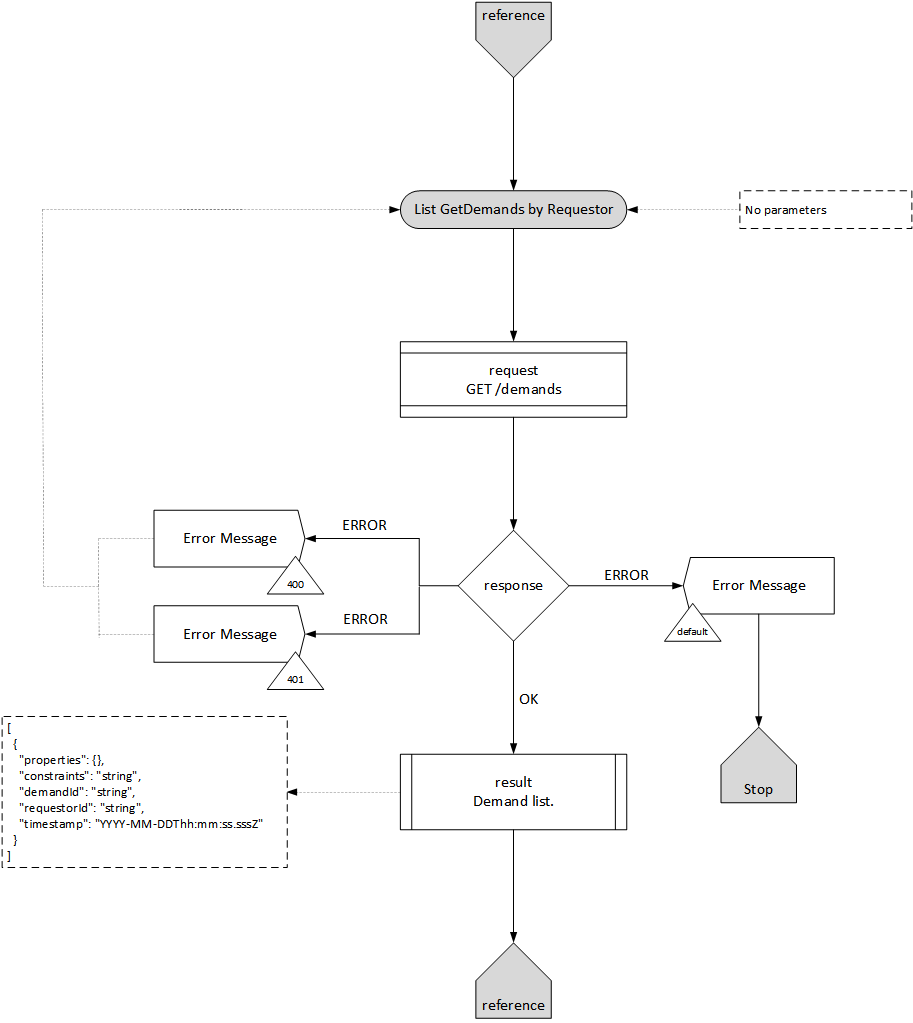
\includegraphics[width=12cm,height=12cm,angle=0]{./diag/Workflow/Market/List(GetDemands)-R-Workflow.png}
    \caption{Requestor Workflow Active Demand List }
	\label{fig:LD}
\end{figure}


\end{enumerate}

\newpage

\subsubsubsubsection{CollectOffers Function}

\begin{enumerate}

\item Profile

\begin{enumerate}

\item Description

The CollectOffers function is used to read Market responses to published Demand by the Requestor.  \\
It uses the GET /demands/\{subscriptionId\}/events method.

\item Side

Requestor

\end{enumerate}

\item Request

\begin{enumerate}

\item Input

\begin{tcolorbox}[boxrule=0pt, frame empty]
\begin{verbatim}

subscriptionId
timeout
maxEvents

\end{verbatim}
\end{tcolorbox}

%Offer Object
%\begin{tcolorbox}[boxrule=0pt, frame empty]
%\begin{verbatim}
%{
%  "properties": {},
%  "constraints": "string"
%}
%\end{verbatim}
%\end{tcolorbox}

\begin{center}
\begin{tabular}{|p{3cm}|l|p{3cm}|p{3cm}|p{4cm}|} 
\hline
\rowcolor{lightgray}	Name	& MO.	& Type	& Example & 	Description \\
\hline

subscriptionId	& M	& 	string			&		&	Subscription Identifier \\ 

\hline

timeout			& O	& 	number(\$float)	&		&	Timeout used in long-polling calls (in seconds). 
													How many seconds server should wait for response containing new events 
													(0.0 means it should return immediately if there are no events).	Default value : 5 \\ 

\hline

maxEvents		& O & integer(\$int32)	&		&	Maximum number of events that server should return at once.		Default value : 10 \\

\hline	

\end{tabular}
\end{center}

\item REST Method

\begin{tcolorbox}[boxrule=0pt, frame empty]
\begin{verbatim} 

GET /demands/{subscriptionId}/events

\end{verbatim}
\end{tcolorbox}

\end{enumerate}

\item Response

\begin{center}
\begin{tabular}{|c|l|} 
\hline
\rowcolor{lightgray}	Code 		& 	Description \\
\hline
200	 		&	Proposal or Agreement event list. \\
\hline
404			&	(404) The specified resource was not found. \\
\hline
401			&	(401) Authorization information is missing or invalid. \\
\hline
default		&	Unexpected error. \\
\hline
\end{tabular}
\end{center}


\item Result

\begin{tcolorbox}[boxrule=0pt, frame empty]
\begin{verbatim}

[
  {
    "eventType": "string",
    "eventDate": "YYYY-MM-DDThh:mm:ss.sssZ"
  }
]

\end{verbatim}
\end{tcolorbox}

\begin{center}
\begin{tabular}{|p{3cm}|l|p{3cm}|p{3cm}|p{4cm}|} 
\hline
\rowcolor{lightgray}	Name	& MO.	& Type	& Example & 	Description \\
\hline

eventType	& 	& 	string	&		&	Event Type \\ 

\hline

eventDate	& 	& 	string(\$date-time)	&	YYYY-MM-DDThh:mm:ss.sssZ	&	Event Date \\ 

\hline

\end{tabular}
\end{center}


\item Workflow

(Please see Figure ~\ref{fig:CO} on page ~\pageref{fig:CO}):

\begin{figure}[htbp]
    \centering
    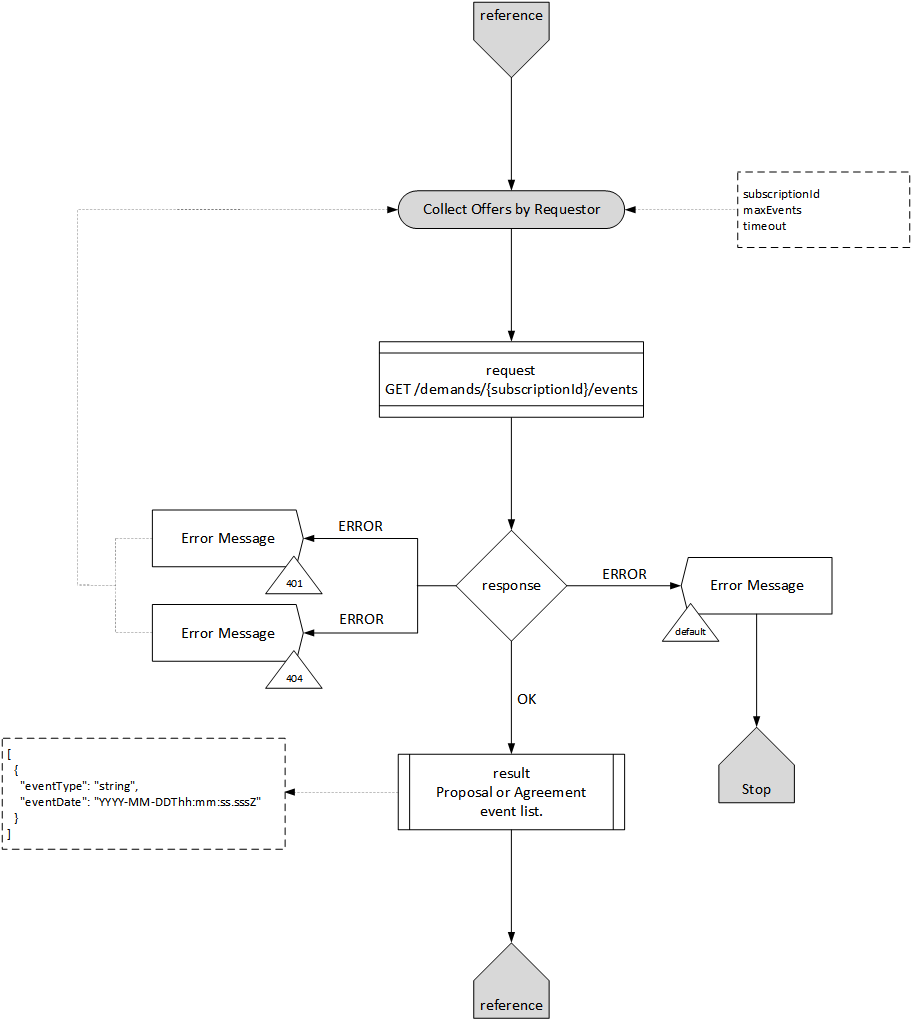
\includegraphics[width=11cm,height=11cm,angle=0]{./diag/Workflow/Market/CollectOffers-R-Workflow.png}
    \caption{Requestor Workflow Collect Offers }
	\label{fig:CO}
\end{figure}


\end{enumerate}

\newpage

\subsubsubsubsection{GetProposalOffer Function}

\begin{enumerate}

\item Profile

\begin{enumerate}

\item Description

The GetProposalOffer function is used to fetch Proposal (Offer) with given id. \\
It uses the GET /demands/\{subscriptionId\}/proposals/\{proposalId\} method.

\item Side

Requestor

\end{enumerate}

\item Request

\begin{enumerate}

\item Input

\begin{tcolorbox}[boxrule=0pt, frame empty]
\begin{verbatim}

subscriptionId
proposalId

\end{verbatim}
\end{tcolorbox}

%Offer Object
%\begin{tcolorbox}[boxrule=0pt, frame empty]
%\begin{verbatim}
%{
%  "properties": {},
%  "constraints": "string"
%}
%\end{verbatim}
%\end{tcolorbox}

\begin{center}
\begin{tabular}{|p{3cm}|l|p{3cm}|p{3cm}|p{4cm}|} 
\hline
\rowcolor{lightgray}	Name	& MO.	& Type	& Example & 	Description \\
\hline

subscriptionId	& M	& 	string			&		&	Subscription Identifier \\ 

\hline

proposalId		& M & 	string			&		&	Proposal Identifier \\

\hline	

\end{tabular}
\end{center}

\item REST Method

\begin{tcolorbox}[boxrule=0pt, frame empty]
\begin{verbatim} 

GET /demands/{subscriptionId}/proposals/{proposalId}

\end{verbatim}
\end{tcolorbox}

\end{enumerate}

\item Response

\begin{center}
\begin{tabular}{|c|l|} 
\hline
\rowcolor{lightgray}	Code 		& 	Description \\
\hline
200	 		&	Proposal  \\
\hline
404			&	(404) The specified resource was not found. \\
\hline
401			&	(401) Authorization information is missing or invalid. \\
\hline
410			&	Proposal rejected. \\
\hline
default		&	Unexpected error. \\
\hline
\end{tabular}
\end{center}


\item Result

\begin{tcolorbox}[boxrule=0pt, frame empty]
\begin{verbatim}

{
  "properties": {},
  "constraints": "string",
  "proposalId": "string",
  "issuerId": "string",
  "state": "Initial",
  "timestamp": "YYYY-MM-DDThh:mm:ss.sssZ",
  "prevProposalId": "string"
}

\end{verbatim}
\end{tcolorbox}

\begin{center}
\begin{tabular}{|p{3cm}|l|p{3cm}|p{3cm}|p{4cm}|} 
\hline
\rowcolor{lightgray}	Name	& MO.	& Type	& Example & 	Description \\
\hline

properties	& 	& 	json or flat		&								&	 \\ 

\hline

constraints &	&	string				&								&	\\

\hline

proposalId	&	&	string				&								& Proposal Identifier \\

\hline

issuerId	&	&	string				&								& Issuer Node Id \\

\hline

state		&	&	enum				& [Initial, Draft, Rejected, Accepted, Expired] & Proposal State \\

\hline

timestamp	& 	& 	string(\$date-time)	&	YYYY-MM-DDThh:mm:ss.sssZ	&	Time ? \\ 

\hline

prevProposalId & &	string 				&								&	Id of the proposal from other side which this proposal responds to \\

\hline

\end{tabular}
\end{center}


\item Workflow

(Please see Figure ~\ref{fig:GPO} on page ~\pageref{fig:GPO}):

\begin{figure}[htbp]
    \centering
    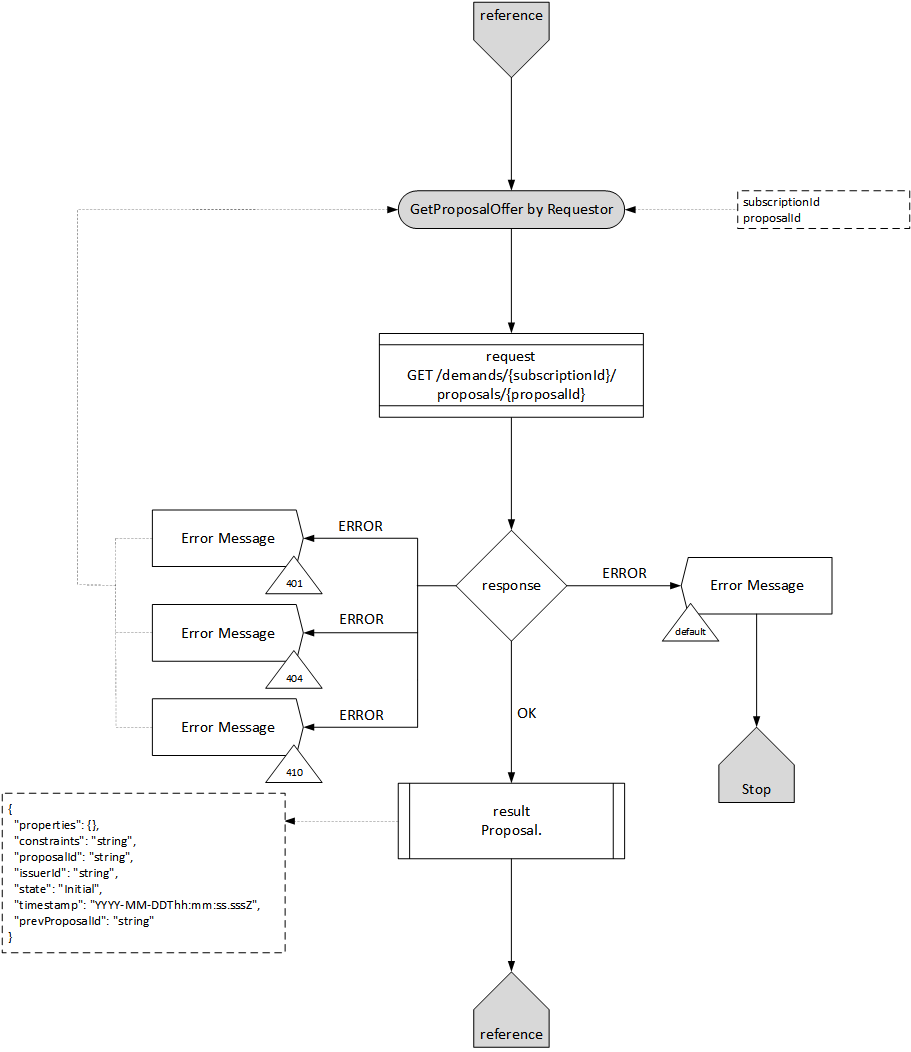
\includegraphics[width=12cm,height=12cm,angle=0]{./diag/Workflow/Market/GetProposalOffer-R-Workflow.png}
    \caption{Requestor Workflow Get Proposal Offer }
	\label{fig:GPO}
\end{figure}


\end{enumerate}

\newpage

\subsubsubsubsection{CounterProposalDemand Function}

\begin{enumerate}

\item Profile

\begin{enumerate}

\item Description

The CounterProposalDemand function is used to respond with bespoke Demand to received Offer. \\
It uses the POST /demands/\{subscriptionId\}/proposals/\{proposalId\} method.

\item Side

Requestor

\end{enumerate}

\item Request

\begin{enumerate}

\item Input

\begin{tcolorbox}[boxrule=0pt, frame empty]
\begin{verbatim}

subscriptionId
proposalId

\end{verbatim}
\end{tcolorbox}

Demand Object
\begin{tcolorbox}[boxrule=0pt, frame empty]
\begin{verbatim}
{
  "properties": {},
  "constraints": "string"
}
\end{verbatim}
\end{tcolorbox}

\begin{center}
\begin{tabular}{|p{3cm}|l|p{3cm}|p{3cm}|p{4cm}|} 
\hline
\rowcolor{lightgray}	Name	& MO.	& Type	& Example & 	Description \\
\hline

subscriptionId	& M	& 	string			&		&	Subscription Identifier \\ 

\hline

proposalId		& M & 	string			&		&	Proposal Identifier \\

\hline	

properties		& M &	json or flat 	&		& Demand Properties		\\

\hline

constraints 	& M &	string			&		& Demand Constraints		\\

\hline

\end{tabular}
\end{center}

\item REST Method

\begin{tcolorbox}[boxrule=0pt, frame empty]
\begin{verbatim} 

POST /demands/{subscriptionId}/proposals/{proposalId}

\end{verbatim}
\end{tcolorbox}

\end{enumerate}

\item Response

\begin{center}
\begin{tabular}{|c|l|} 
\hline
\rowcolor{lightgray}	Code 		& 	Description \\
\hline
201	 		&	Counter Proposal created.  \\
\hline
400			&	(400) Bad request	\\
\hline
404			&	(404) The specified resource was not found. \\
\hline
401			&	(401) Authorization information is missing or invalid. \\
\hline
410			&	Proposal rejected. \\
\hline
default		&	Unexpected error. \\
\hline
\end{tabular}
\end{center}


\item Result

\begin{tcolorbox}[boxrule=0pt, frame empty]
\begin{verbatim}
  proposalId
\end{verbatim}
\end{tcolorbox}

\begin{center}
\begin{tabular}{|p{3cm}|l|p{3cm}|p{3cm}|p{4cm}|} 
\hline
\rowcolor{lightgray}	Name	& MO.	& Type	& Example & 	Description \\
\hline

proposalId	&	&	string				&								& Proposal Identifier \\

\hline

\end{tabular}
\end{center}


\item Workflow

(Please see Figure ~\ref{fig:CPD} on page ~\pageref{fig:CPD}):

\begin{figure}[htbp]
    \centering
    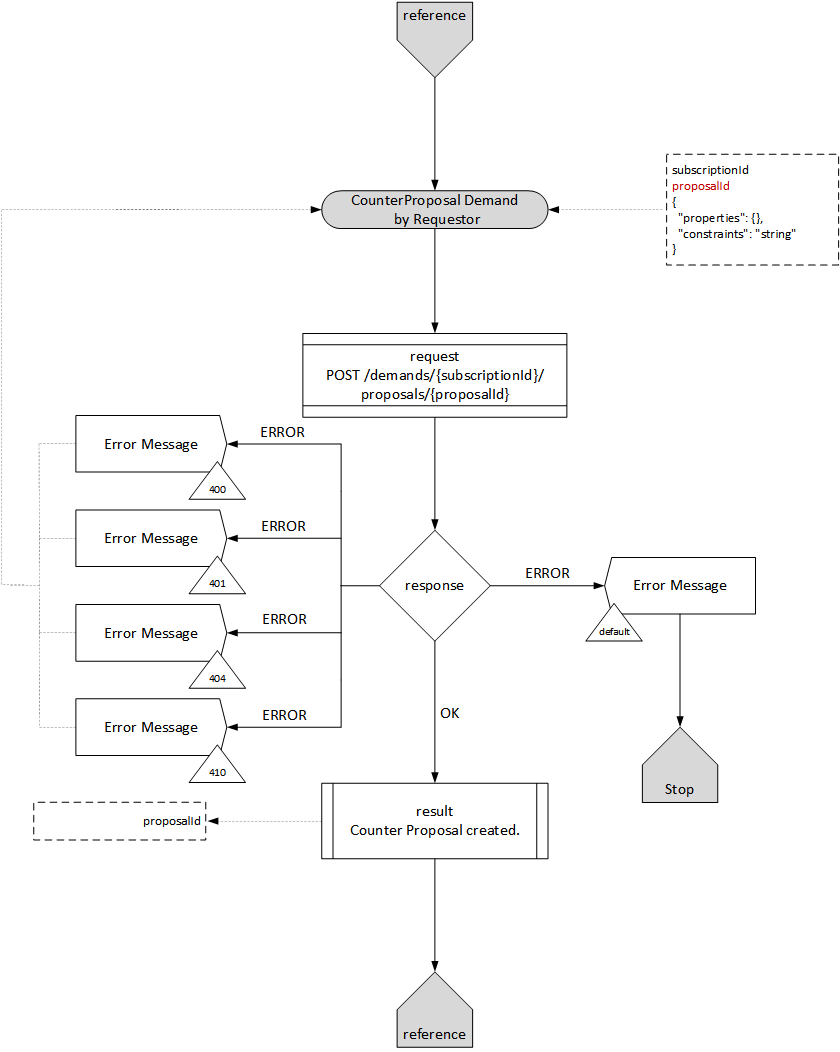
\includegraphics[width=12cm,height=12cm,angle=0]{./diag/Workflow/Market/CounterProposalDemand-R-Workflow.png}
    \caption{Requestor Workflow Counter Proposal Demand }
	\label{fig:CPD}
\end{figure}


\end{enumerate}

\newpage

\subsubsubsubsection{RejectProposalOffer Function}

\begin{enumerate}

\item Profile

\begin{enumerate}

\item Description

The RejectProposalOffer function is used to reject Proposal Offer. \\
It uses the POST /demands/\{subscriptionId\}/proposals/\{proposalId\}/reject method.

\item Side

Requestor

\end{enumerate}

\item Request

\begin{enumerate}

\item Input

\begin{tcolorbox}[boxrule=0pt, frame empty]
\begin{verbatim}

subscriptionId
proposalId

\end{verbatim}
\end{tcolorbox}

Object
\begin{tcolorbox}[boxrule=0pt, frame empty]
\begin{verbatim}
{
  "message": "string",
  "additionalProp1": {}
}
\end{verbatim}
\end{tcolorbox}

\begin{center}
\begin{tabular}{|p{3cm}|l|p{3cm}|p{3cm}|p{4cm}|} 
\hline
\rowcolor{lightgray}	Name	& MO.	& Type	& Example & 	Description \\
\hline

subscriptionId		& M	& 	string			&		&	Subscription Identifier \\ 

\hline

proposalId			& M & 	string			&		&	Proposal Identifier \\

\hline	

message				& O &	string 			&		& 		\\

\hline

additionalProp1 	& O &	json			&		& 		\\

\hline

\end{tabular}
\end{center}

\item REST Method

\begin{tcolorbox}[boxrule=0pt, frame empty]
\begin{verbatim} 

POST /demands/{subscriptionId}/proposals/{proposalId}/reject

\end{verbatim}
\end{tcolorbox}

\end{enumerate}

\item Response

\begin{center}
\begin{tabular}{|c|l|} 
\hline
\rowcolor{lightgray}	Code 		& 	Description \\
\hline
204	 		&	Proposal rejected.  \\
\hline
404			&	(404) The specified resource was not found. \\
\hline
401			&	(401) Authorization information is missing or invalid. \\
\hline
410			&	Proposal rejected. \\
\hline
default		&	Unexpected error. \\
\hline
\end{tabular}
\end{center}


\item Result

\begin{tcolorbox}[boxrule=0pt, frame empty]
\begin{verbatim}
  None
\end{verbatim}
\end{tcolorbox}

\item Workflow

(Please see Figure ~\ref{fig:RPO} on page ~\pageref{fig:RPO}):

\begin{figure}[htbp]
    \centering
    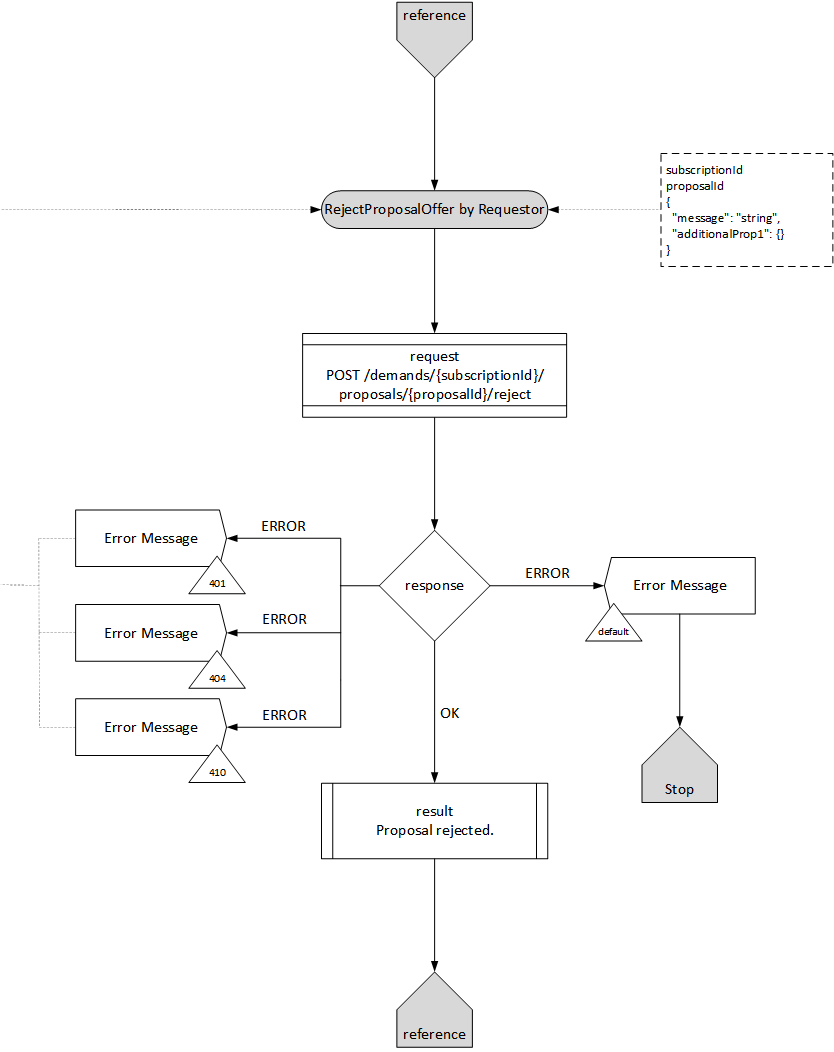
\includegraphics[width=12cm,height=12cm,angle=0]{./diag/Workflow/Market/RejectProposalOffer-R-Workflow.png}
    \caption{Requestor Workflow Reject Proposal Offer }
	\label{fig:RPO}
\end{figure}


\end{enumerate}

\newpage

\subsubsubsubsection{ListAgreements Function}

\begin{enumerate}

\item Profile

\begin{enumerate}

\item Description

The ListAgreements function is used to list Agreement objects with optional filters by the Requestor and Provider node. 
It uses the GET /agreements method.

\item Side

Both

\end{enumerate}

\item Request

\begin{enumerate}

\item Input

\begin{tcolorbox}[boxrule=0pt, frame empty]
\begin{verbatim}

appSessionId
state
afterTimestamp
beforeTimestamp

\end{verbatim}
\end{tcolorbox}

Object
\begin{tcolorbox}[boxrule=0pt, frame empty]
\begin{verbatim}
{
  "proposalId": "string",
  "validTo": "YYYY-MM-DDThh:mm:ss.sssZ"
}
\end{verbatim}
\end{tcolorbox}

\begin{center}
\begin{tabular}{|p{3cm}|l|p{3cm}|p{3cm}|p{4cm}|} 
\hline
\rowcolor{lightgray}	Name	& MO.	& Type	& Example & 	Description \\
\hline

appSessionId	& O & 	string				&			& A correlation/session identifier used for querying events related to an action where this appSessionId has been specified \\
\hline

state			& O	& 	string(enum)		&	[Proposal, Pending, Cancelled, Rejected, Approved, Expired, Terminated]	&	State of an agreement \\ 
\hline

afterTimestamp	& O &	string(\$date-time)	&	YYYY-MM-DDThh:mm:ss.sssZ	&	Apply only to records created later than the specified timestamp \\
\hline

beforeTimestamp	& O &	string(\$date-time)	&	YYYY-MM-DDThh:mm:ss.sssZ	&	Apply only to records created before the specified timestamp \\
\hline

\end{tabular}
\end{center}

\item REST Method

\begin{tcolorbox}[boxrule=0pt, frame empty]
\begin{verbatim} 

GET /agreements

\end{verbatim}
\end{tcolorbox}

\end{enumerate}

\item Response

\begin{center}
\begin{tabular}{|c|l|} 
\hline
\rowcolor{lightgray}	Code 		& 	Description \\
\hline
200	 		&	Result of listing agreements. \\
\hline
400			&	(400) Bad request \\
\hline
401			&	(401) Authorization information is missing or invalid. \\
\hline
default		&	Unexpected error. \\
\hline
\end{tabular}
\end{center}


\item Result

\begin{tcolorbox}[boxrule=0pt, frame empty]
\begin{verbatim}

[
  {
    "id": "string",
    "timestamp": "YYYY-MM-DDThh:mm:ss.sssZ",
    "approvedDate": "YYYY-MM-DDThh:mm:ss.sssZ",
    "role": "string"
  }
]

\end{verbatim}
\end{tcolorbox}

\begin{center}
\begin{tabular}{|p{3cm}|l|p{3cm}|p{3cm}|p{4cm}|} 
\hline
\rowcolor{lightgray}	Name	& MO.	& Type	& Example & 	Description \\
\hline

id				& 	& 	string				&								&	Agreement Identyfier \\ 
\hline

timestamp		& 	& 	string(\$date-time)	&	YYYY-MM-DDThh:mm:ss.sssZ	&	 \\ 
\hline

approvedDate	& 	& 	string(\$date-time)	&	YYYY-MM-DDThh:mm:ss.sssZ	&	 \\ 
\hline

role			& 	& 	string				&								&	 \\ 
\hline

\end{tabular}
\end{center}


\item Workflow

(Please see Figure ~\ref{fig:BLA} on page ~\pageref{fig:BLA}):

\begin{figure}[htbp]
    \centering
    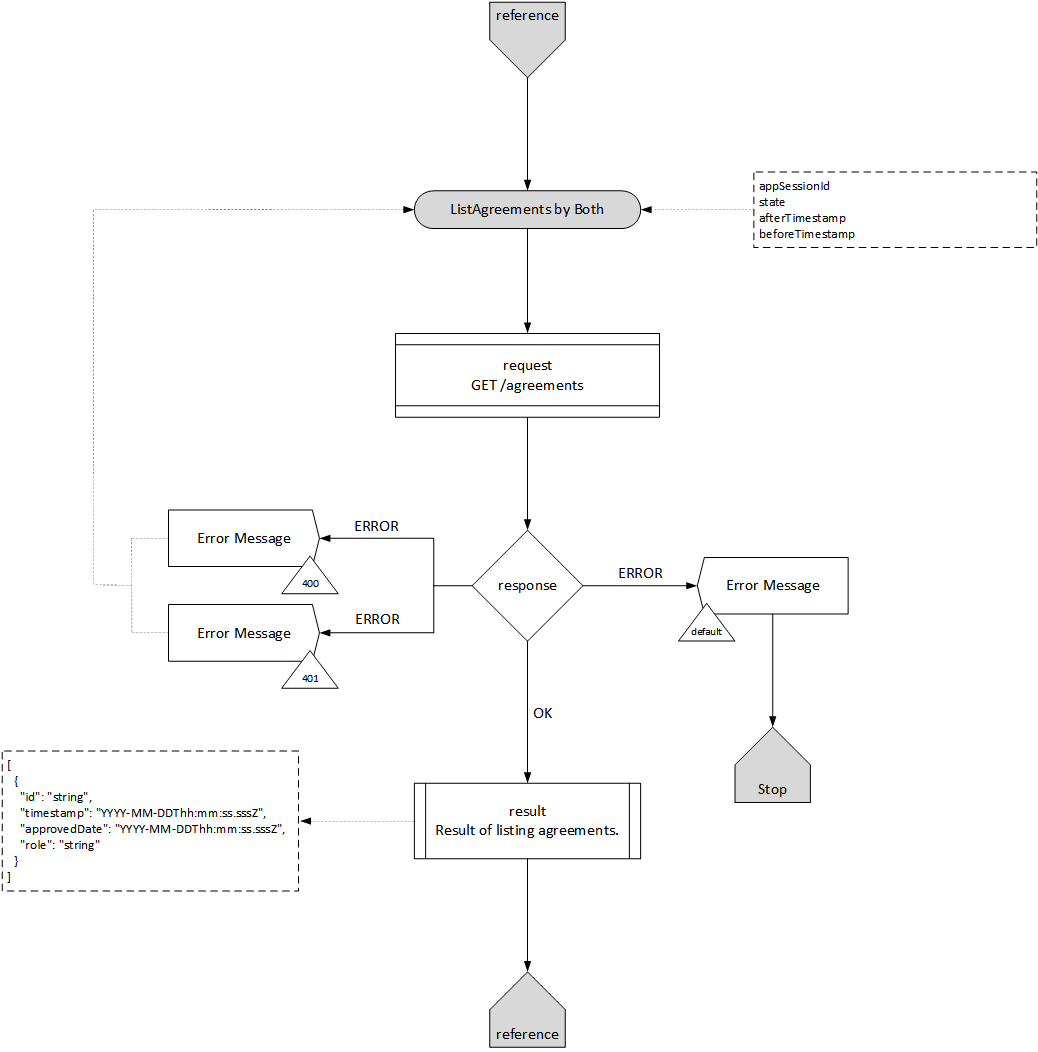
\includegraphics[width=11cm,height=11cm,angle=0]{./diag/Workflow/Market/ListAgreements-B-Workflow.png}
    \caption{Both Workflow List Agreements }
	\label{fig:BLA}
\end{figure}

\end{enumerate}

\newpage

\subsubsubsubsection{GetAgreement Function}

\begin{enumerate}

\item Profile

\begin{enumerate}

\item Description

The GetAgreement function is used to fetch Agreement objects with given agreementId by the Requestor and Provider node. 
It uses the GET /agreements/\{agreementId\} method.

\item Side

Both

\end{enumerate}

\item Request

\begin{enumerate}

\item Input

\begin{tcolorbox}[boxrule=0pt, frame empty]
\begin{verbatim}

agreementId

\end{verbatim}
\end{tcolorbox}

%Object
%\begin{tcolorbox}[boxrule=0pt, frame empty]
%\begin{verbatim}
%{
%  "proposalId": "string",
%  "validTo": "YYYY-MM-DDThh:mm:ss.sssZ"
%}
%\end{verbatim}
%\end{tcolorbox}

\begin{center}
\begin{tabular}{|p{3cm}|l|p{3cm}|p{3cm}|p{4cm}|} 
\hline
\rowcolor{lightgray}	Name	& MO.	& Type	& Example & 	Description \\
\hline

agreementId	& M & 	string				&			& Agreement Identifier \\
\hline

\end{tabular}
\end{center}

\item REST Method

\begin{tcolorbox}[boxrule=0pt, frame empty]
\begin{verbatim} 

GET /agreements/agreementId

\end{verbatim}
\end{tcolorbox}

\end{enumerate}

\item Response

\begin{center}
\begin{tabular}{|c|l|} 
\hline
\rowcolor{lightgray}	Code 		& 	Description \\
\hline
200	 		&	Agreement. \\
\hline
404			&	(404) The specified resource was not found. \\
\hline
401			&	(401) Authorization information is missing or invalid. \\
\hline
default		&	Unexpected error. \\
\hline
\end{tabular}
\end{center}


\item Result

\begin{tcolorbox}[boxrule=0pt, frame empty]
\begin{verbatim}

{
  "agreementId": "string",
  "demand": {
    "properties": {},
    "constraints": "string",
    "demandId": "string",
    "requestorId": "string",
    "timestamp": "YYYY-MM-DDThh-MM-DDThh:mm:ss.sssZ"
  },
  "offer": {
    "properties": {},
    "constraints": "string",
    "offerId": "string",
    "providerId": "string",
    "timestamp": "YYYY-MM-DDThh-MM-DDThh:mm:ss.sssZ"
  },
  "validTo": "YYYY-MM-DDThh-MM-DDThh:mm:ss.sssZ",
  "approvedDate": "YYYY-MM-DDThh-MM-DDThh:mm:ss.sssZ",
  "state": "Proposal",
  "timestamp": "YYYY-MM-DDThh-MM-DDThh:mm:ss.sssZ",
  "appSessionId": "string",
  "proposedSignature": "string",
  "approvedSignature": "string",
  "committedSignature": "string"
}

\end{verbatim}
\end{tcolorbox}

\begin{center}
\begin{tabular}{|p{3cm}|l|p{3cm}|p{3cm}|p{4cm}|} 
\hline
\rowcolor{lightgray}	Name	& MO.	& Type	& Example & 	Description \\
\hline

agreementId				& 	& 	string				&		&	Agreement Identyfier \\ 
\hline

demand.properties		&	&	json or flat		&		& 	Demand Properties \\
\hline

demand.constraints		&	&	string				&		&	Demand Constraints \\	
\hline

demand.demandId			&	&	string				&		&	Demand Identifier \\
\hline 		

demand.requestorId		&	&	string 				&		&	Requestor Node Identifier \\
\hline

demand.timestamp		& 	& 	string(\$date-time)	&	YYYY-MM-DDThh:mm:ss.sssZ	&	 \\ 
\hline

offer.properties		&	&	json or flat		&		& 	Offer Properties \\
\hline

offer.constraints		&	&	string				&		&	Offer Constraints \\	
\hline

offer.offerId			&	&	string				&		&	Offer Identifier \\
\hline 		

offer.providerId		&	&	string 				&		&	Provider Node Identifier \\
\hline

offer.timestamp		& 	& 	string(\$date-time)	&	YYYY-MM-DDThh:mm:ss.sssZ	&	 \\ 
\hline

validTo			& 	& 	string(\$date-time)	&	YYYY-MM-DDThh:mm:ss.sssZ	&	 \\ 
\hline

approvedDate	& 	& 	string(\$date-time)	&	YYYY-MM-DDThh:mm:ss.sssZ	&	 \\ 
\hline

state			& 	& 	string(enum)		&	[ Proposal, Pending, Cancelled, Rejected, Approved, Expired, Terminated ]	& Agreement State	\\ 
\hline

timestamp		& 	& 	string(\$date-time)	&	YYYY-MM-DDThh:mm:ss.sssZ	&	 \\ 
\hline

appSessionId	&	&	string 				&			&	AppSessionId \\
\hline

proposedSignature &		& string 			&			&	Proposed Signature \\
\hline

approvedSignature &		&  string			&			&  Approved Signature \\
\hline  
  
committedSignature &	& 	string			&			&	Committed Signature \\
\hline

\end{tabular}
\end{center}


\item Workflow

(Please see Figure ~\ref{fig:BGA} on page ~\pageref{fig:BGA}):

\begin{figure}[htbp]
    \centering
    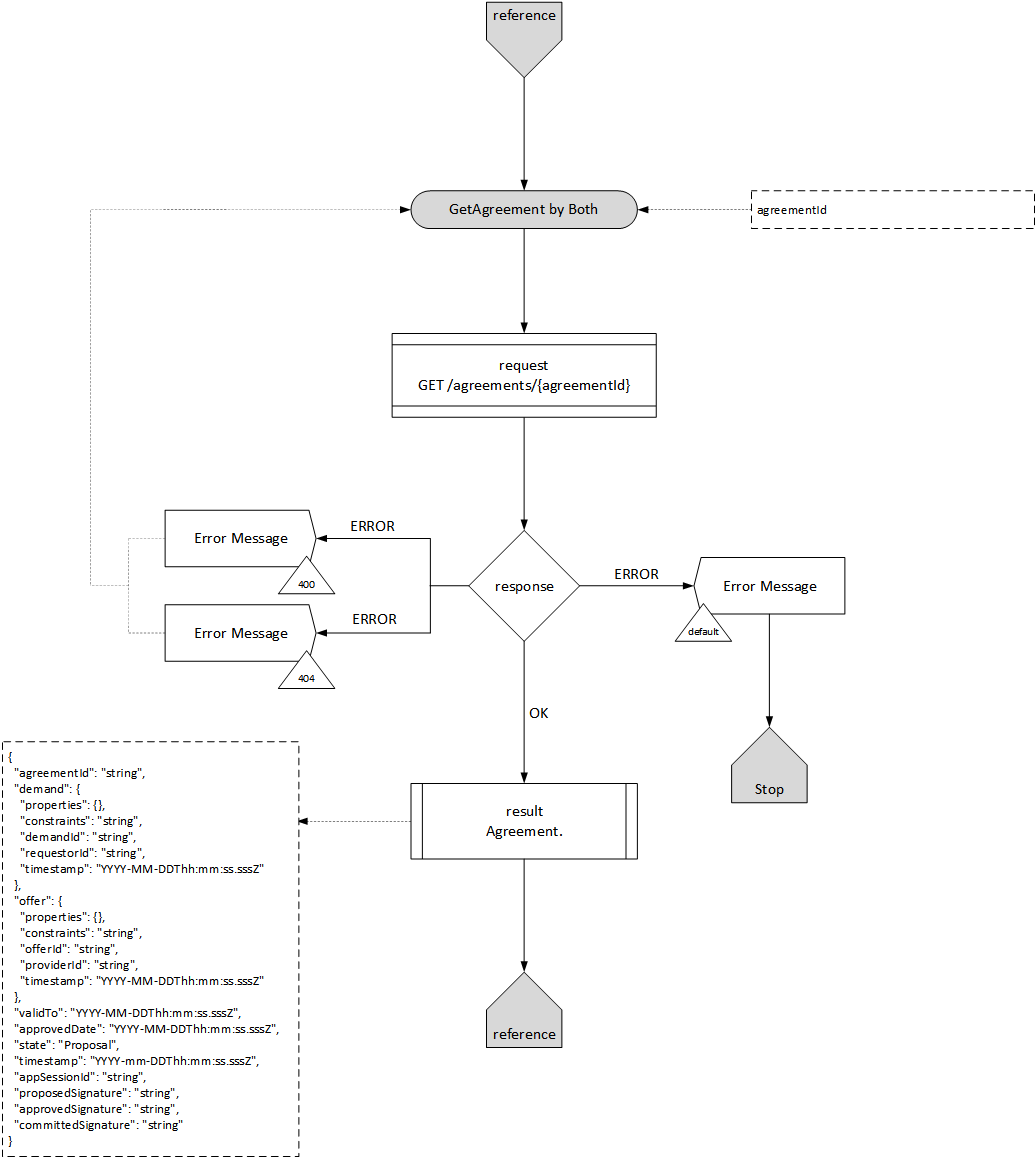
\includegraphics[width=11cm,height=11cm,angle=0]{./diag/Workflow/Market/GetAgreement-B-Workflow.png}
    \caption{Both Workflow Get Agreement }
	\label{fig:BGA}
\end{figure}

\end{enumerate}

\newpage

% AgreementEvents
\subsubsubsubsection{CollectAgreementEvents Function}

\begin{enumerate}

\item Profile

\begin{enumerate}

\item Description

The CollectAgreementEvents function is used to collect events related to an Agreement objects with optional filters by the Requestor and Provider node. 
It uses the GET /agreementEvents method.

\item Side

Both

\end{enumerate}

\item Request

\begin{enumerate}

\item Input

\begin{tcolorbox}[boxrule=0pt, frame empty]
\begin{verbatim}

appSessionId
maxEvents
afterTimestamp
timeout

\end{verbatim}
\end{tcolorbox}

%Object
%\begin{tcolorbox}[boxrule=0pt, frame empty]
%\begin{verbatim}
%{
%  "proposalId": "string",
%  "validTo": "YYYY-MM-DDThh:mm:ss.sssZ"
%}
%\end{verbatim}
%\end{tcolorbox}

\begin{center}
\begin{tabular}{|p{3cm}|l|p{3cm}|p{3cm}|p{4cm}|} 
\hline
\rowcolor{lightgray}	Name	& MO.	& Type	& Example & 	Description \\
\hline

appSessionId	& O & 	string				&			& A correlation/session identifier used for querying events related to an action where this appSessionId has been specified \\
\hline

maxEvents			& O	& 	integer(\$int32)		&	10	&	Maximum number of events that server should return at once. \\ 
\hline

afterTimestamp	& O &	string(\$date-time)	&	YYYY-MM-DDThh:mm:ss.sssZ	&	Apply only to records created later than the specified timestamp \\
\hline

timeout	& O &	number(\$float)	&	5	&	Timeout used in long-polling calls (in seconds). 
											How many seconds server should wait for response containing new events 
											(0.0 means it should return immediately if there are no events) \\
\hline

\end{tabular}
\end{center}

\item REST Method

\begin{tcolorbox}[boxrule=0pt, frame empty]
\begin{verbatim} 

GET /agreementEvents

\end{verbatim}
\end{tcolorbox}

\end{enumerate}

\item Response

\begin{center}
\begin{tabular}{|c|l|} 
\hline
\rowcolor{lightgray}	Code 		& 	Description \\
\hline
200	 		&	Agreement-related event list. \\
\hline
400			&	(400) Bad request \\
\hline
401			&	(401) Authorization information is missing or invalid. \\
\hline
default		&	Unexpected error. \\
\hline
\end{tabular}
\end{center}


\item Result

\begin{tcolorbox}[boxrule=0pt, frame empty]
\begin{verbatim}

[
  {
    "eventType": "string",
    "eventDate": "YYYY-MM-DDThh:mm:ss.sssZ",
    "agreementId": "string"
  }
]

\end{verbatim}
\end{tcolorbox}

\begin{center}
\begin{tabular}{|p{3cm}|l|p{3cm}|p{3cm}|p{4cm}|} 
\hline
\rowcolor{lightgray}	Name	& MO.	& Type	& Example & 	Description \\
\hline

agreementId		& 	& 	string				&						&	Agreement Identyfier \\ 
\hline

eventDate		& 	& 	string(\$date-time)	&	YYYY-MM-DDThh:mm:ss.sssZ	&	 \\ 
\hline

eventType		& 	& 	string(enum)		&	[AgreementApprovedEvent, AgreementRejectedEvent, AgreementCancelledEvent, AgreementTerminatedEvent] &	Event Type \\ 
\hline

\end{tabular}
\end{center}


\item Workflow

(Please see Figure ~\ref{fig:CAE} on page ~\pageref{fig:CAE}):

\begin{figure}[htbp]
    \centering
    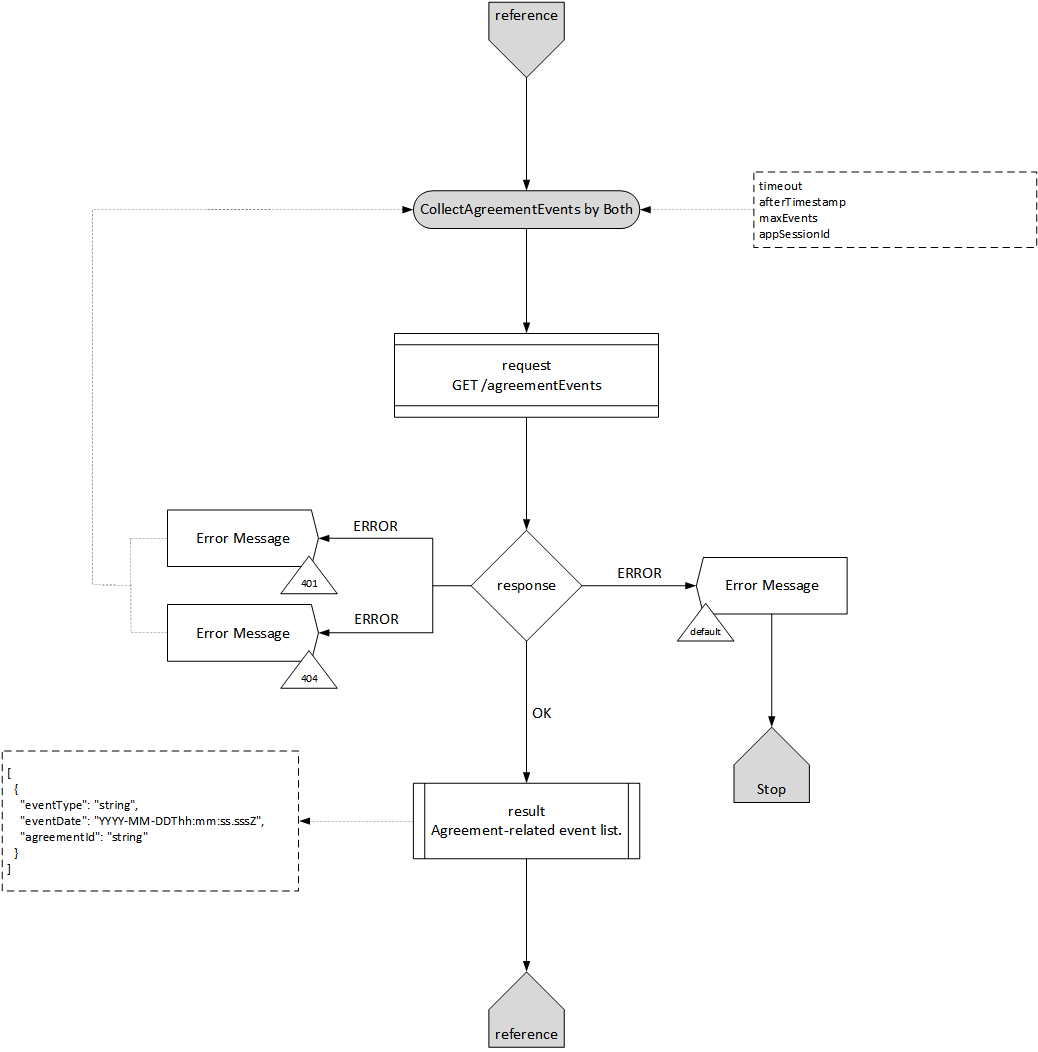
\includegraphics[width=11cm,height=11cm,angle=0]{./diag/Workflow/Market/CollectAgreementEvents-B-Workflow.png}
    \caption{Both Workflow Collect Agreement Events }
	\label{fig:CAE}
\end{figure}

\end{enumerate}

\newpage

% TerminateAgreement
\subsubsubsubsection{TerminateAgreement Function}

\begin{enumerate}

\item Profile

\begin{enumerate}

\item Description

The TerminateAgreement function is used to terminate approved Agreement objects by the Requestor and Provider node. 
It uses the POST /agreements/\{agreementId\}/terminate method.

\item Side

Both

\end{enumerate}

\item Request

\begin{enumerate}

\item Input

\begin{tcolorbox}[boxrule=0pt, frame empty]
\begin{verbatim}

agreementId

\end{verbatim}
\end{tcolorbox}

Object
\begin{tcolorbox}[boxrule=0pt, frame empty]
\begin{verbatim}
{
  "message": "string",
  "additionalProp1": {}
}
\end{verbatim}
\end{tcolorbox}

\begin{center}
\begin{tabular}{|p{3cm}|l|p{3cm}|p{3cm}|p{4cm}|} 
\hline
\rowcolor{lightgray}	Name	& MO.	& Type	& Example & 	Description \\
\hline

agreementId		& M & 	string				&		& 	Agreement Identifier \\
\hline

message			& O	& 	string				&		&	 	\\ 
\hline

additionalProp1	& O &	json				&		&		\\
\hline

\end{tabular}
\end{center}

\item REST Method

\begin{tcolorbox}[boxrule=0pt, frame empty]
\begin{verbatim} 

POST /agreements/{agreementId}/terminate

\end{verbatim}
\end{tcolorbox}

\end{enumerate}

\item Response

\begin{center}
\begin{tabular}{|c|l|} 
\hline
\rowcolor{lightgray}	Code 		& 	Description \\
\hline
204	 		&	Agreement terminated. \\
\hline
404			&	(404) The specified resource was not found. \\
\hline
401			&	(401) Authorization information is missing or invalid. \\
\hline
409			&	(409) Conflict. \\
\hline
410			&	(410) Gone \\
\hline
default		&	Unexpected error. \\
\hline
\end{tabular}
\end{center}

\item Result

\begin{tcolorbox}[boxrule=0pt, frame empty]
\begin{verbatim}

None

\end{verbatim}
\end{tcolorbox}

%\begin{center}
%\begin{tabular}{|p{3cm}|l|p{3cm}|p{3cm}|p{4cm}|} 
%\hline
%\rowcolor{lightgray}	Name	& MO.	& Type	& Example & 	Description \\
%\hline
%agreementId		& 	& 	string				&						&	Agreement Identyfier \\ 
%\hline
%eventDate		& 	& 	string(\$date-time)	&	YYYY-MM-DDThh:mm:ss.sssZ	&	 \\ 
%\hline
%eventType		& 	& 	string(enum)		&	 &	Event Type \\ 
%\hline
%\end{tabular}
%\end{center}

\item Workflow

(Please see Figure ~\ref{fig:BTA} on page ~\pageref{fig:BTA}):

\begin{figure}[htbp]
    \centering
    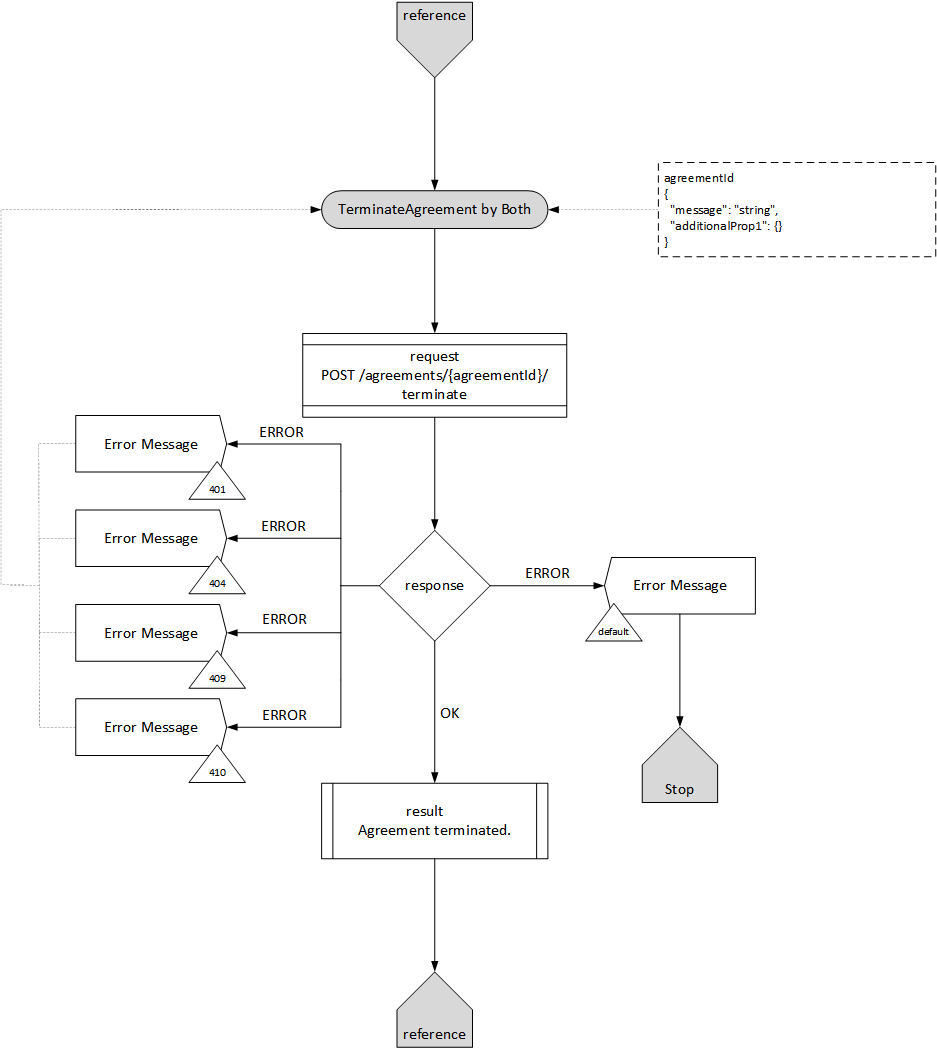
\includegraphics[width=11cm,height=11cm,angle=0]{./diag/Workflow/Market/TerminateAgreement-B-Workflow.png}
    \caption{Both Workflow Terminate Agreement  }
	\label{fig:BTA}
\end{figure}

\end{enumerate}

\newpage

% ReasonTerminateAgreement
\subsubsubsubsection{ReasonTerminateAgreement Function}

\begin{enumerate}

\item Profile

\begin{enumerate}

\item Description

The ReasonTerminateAgreement function is used to get termination reason reported when terminateAgreement was called. 
This method is used by the Requestor and Provider node. It uses the POST /agreements/\{agreementId\}/terminate/reason method.

\item Side

Both

\end{enumerate}

\item Request

\begin{enumerate}

\item Input

\begin{tcolorbox}[boxrule=0pt, frame empty]
\begin{verbatim}

agreementId

\end{verbatim}
\end{tcolorbox}

%Object
%\begin{tcolorbox}[boxrule=0pt, frame empty]
%\begin{verbatim}
%agreementId
%
%\end{verbatim}
%\end{tcolorbox}

\begin{center}
\begin{tabular}{|p{3cm}|l|p{3cm}|p{3cm}|p{4cm}|} 
\hline
\rowcolor{lightgray}	Name	& MO.	& Type	& Example & 	Description \\
\hline
agreementId		& M & 	string				&		& 	Agreement Identifier \\
\hline
\end{tabular}
\end{center}

\item REST Method

\begin{tcolorbox}[boxrule=0pt, frame empty]
\begin{verbatim} 

POST /agreements/{agreementId}/terminate/reason

\end{verbatim}
\end{tcolorbox}

\end{enumerate}

\item Response

\begin{center}
\begin{tabular}{|c|l|} 
\hline
\rowcolor{lightgray}	Code 		& 	Description \\
\hline
200	 		&	Agreement termination reason. \\
\hline
404			&	(404) The specified resource was not found. \\
\hline
401			&	(401) Authorization information is missing or invalid. \\
\hline
400			&	(400) Bad request \\
\hline
default		&	Unexpected error. \\
\hline
\end{tabular}
\end{center}

\item Result

\begin{tcolorbox}[boxrule=0pt, frame empty]
\begin{verbatim}

{
  "eventType": "string",
  "eventDate": "YYYY-MM-DDThh:mm:ss.sssZ",
  "agreementId": "string",
  "terminator": "Requestor",
  "signature": "string",
  "reason": {
    "message": "string",
    "additionalProp1": {}
  }
}

\end{verbatim}
\end{tcolorbox}

\begin{center}
\begin{tabular}{|p{3cm}|l|p{3cm}|p{3cm}|p{4cm}|} 
\hline
\rowcolor{lightgray}	Name	& MO.	& Type	& Example & 	Description \\
\hline
agreementId		& 	& 	string				&								&	Agreement Identyfier \\ 
\hline
eventDate		& 	& 	string(\$date-time)	&	YYYY-MM-DDThh:mm:ss.sssZ	&	 \\ 
\hline
eventType		& 	& 	string(enum)		&	[AgreementApprovedEvent, AgreementRejectedEvent, AgreementCancelledEvent, AgreementTerminatedEvent] &	Event Type \\ 
\hline
terminator 		&	&	enum 				& [Requestor, Provider]			&				\\
\hline
signature 		&	&	string 				&								&				\\
\hline
reason.message 	&	&	string 				&								&				\\
\hline
reason.additionalProp1	&	&	json 			&								&				\\
\hline

\end{tabular}
\end{center}

\item Workflow

(Please see Figure ~\ref{fig:BRTA} on page ~\pageref{fig:BRTA}):

\begin{figure}[htbp]
    \centering
    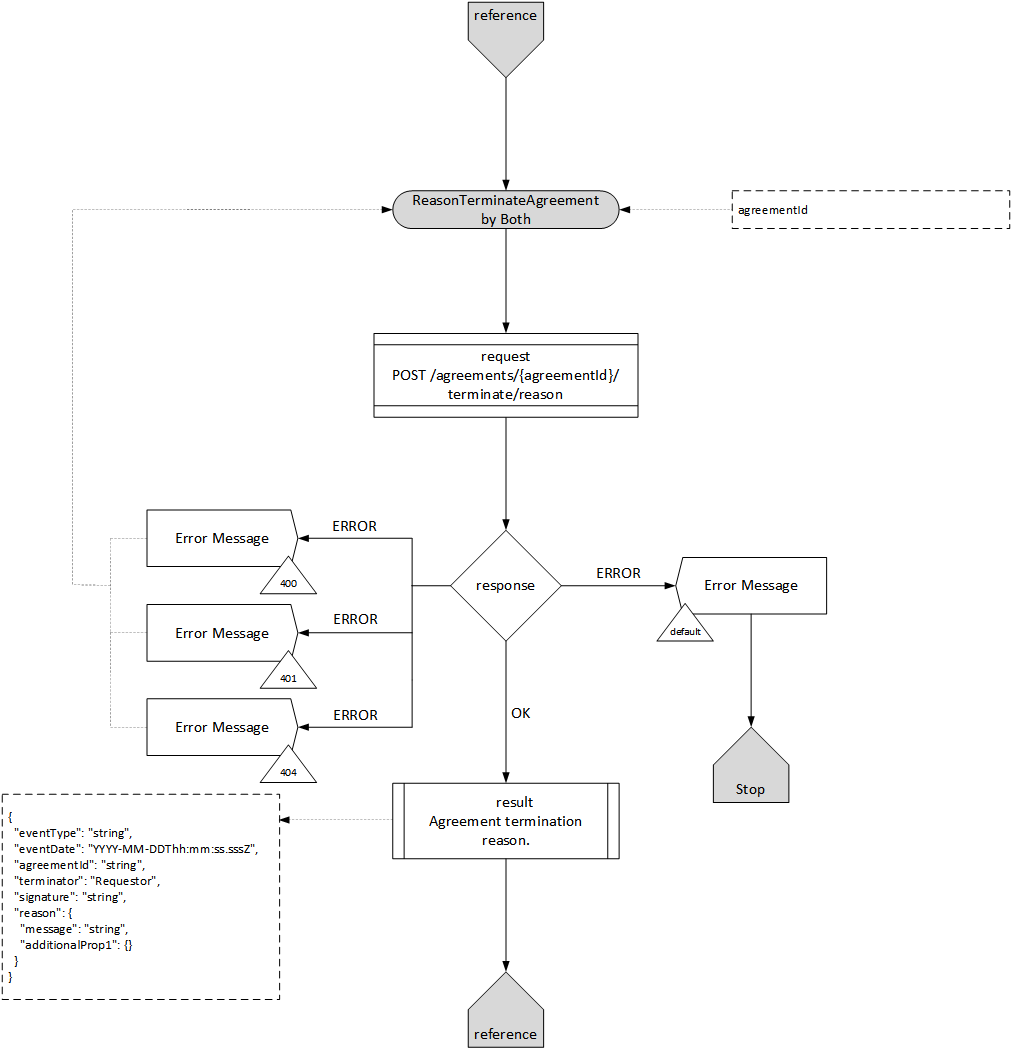
\includegraphics[width=11cm,height=11cm,angle=0]{./diag/Workflow/Market/ReasonTerminateAgreement-B-Workflow.png}
    \caption{Both Workflow Reason Terminate Agreement  }
	\label{fig:BRTA}
\end{figure}

\end{enumerate}

\newpage

% ConfirmAgreement

\subsubsubsubsection{ConfirmAgreement Function}

\begin{enumerate}

\item Profile

\begin{enumerate}

\item Description

The ConfirmAgreement function is used to send Agreement proposal object to the Provider by the Requestor node. 
It uses the POST /agreements/\{agreementId\}/confirm method.

\item Side

Requestor

\end{enumerate}

\item Request

\begin{enumerate}

\item Input

\begin{tcolorbox}[boxrule=0pt, frame empty]
\begin{verbatim}

agreementId
appSessionId

\end{verbatim}
\end{tcolorbox}

%Object
%\begin{tcolorbox}[boxrule=0pt, frame empty]
%\begin{verbatim}
%{
%  "message": "string",
%  "additionalProp1": {}
%}
%\end{verbatim}
%\end{tcolorbox}

\begin{center}
\begin{tabular}{|p{3cm}|l|p{3cm}|p{3cm}|p{4cm}|} 
\hline
\rowcolor{lightgray}	Name	& MO.	& Type	& Example & 	Description \\
\hline

agreementId		& M & 	string				&		& 	Agreement Identifier \\
\hline

appSessionId	& O	& 	string				&		&	A correlation/session identifier used for querying events related to an action where this appSessionId has been specified 	\\ 
\hline

\end{tabular}
\end{center}

\item REST Method

\begin{tcolorbox}[boxrule=0pt, frame empty]
\begin{verbatim} 

POST /agreements/{agreementId}/confirm

\end{verbatim}
\end{tcolorbox}

\end{enumerate}

\item Response

\begin{center}
\begin{tabular}{|c|l|} 
\hline
\rowcolor{lightgray}	Code 		& 	Description \\
\hline
204	 		&	Agreement confirmed. \\
\hline
404			&	(404) The specified resource was not found. \\
\hline
401			&	(401) Authorization information is missing or invalid. \\
\hline
410			&	(410) Gone \\
\hline
default		&	Unexpected error. \\
\hline
\end{tabular}
\end{center}

\item Result

\begin{tcolorbox}[boxrule=0pt, frame empty]
\begin{verbatim}

None

\end{verbatim}
\end{tcolorbox}

%\begin{center}
%\begin{tabular}{|p{3cm}|l|p{3cm}|p{3cm}|p{4cm}|} 
%\hline
%\rowcolor{lightgray}	Name	& MO.	& Type	& Example & 	Description \\
%\hline
%agreementId		& 	& 	string				&						&	Agreement Identyfier \\ 
%\hline
%eventDate		& 	& 	string(\$date-time)	&	YYYY-MM-DDThh:mm:ss.sssZ	&	 \\ 
%\hline
%eventType		& 	& 	string(enum)		&	 &	Event Type \\ 
%\hline
%\end{tabular}
%\end{center}

\item Workflow

(Please see Figure ~\ref{fig:RCA} on page ~\pageref{fig:RCA}):

\begin{figure}[htbp]
    \centering
    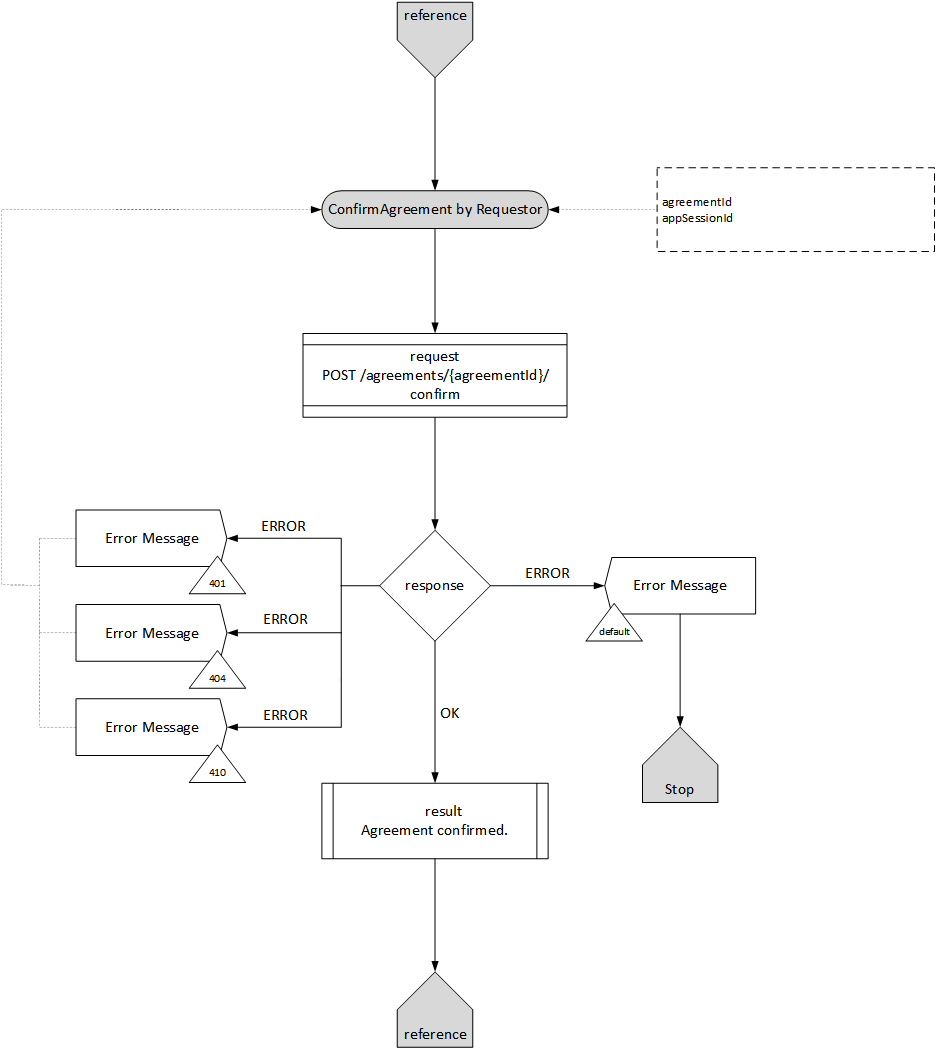
\includegraphics[width=11cm,height=11cm,angle=0]{./diag/Workflow/Market/ConfirmAgreement-R-Workflow.png}
    \caption{Requestor Workflow Confirm Agreement  }
	\label{fig:RCA}
\end{figure}

\end{enumerate}

\newpage

% CancelAgreement

\subsubsubsubsection{CancelAgreement Function}

\begin{enumerate}

\item Profile

\begin{enumerate}

\item Description

The CancelAgreement function is used to cancel Agreement object by the Requestor node. 
It uses the POST /agreements/\{agreementId\}/cancel method.

\item Side

Requestor

\end{enumerate}

\item Request

\begin{enumerate}

\item Input

\begin{tcolorbox}[boxrule=0pt, frame empty]
\begin{verbatim}

agreementId
appSessionId

\end{verbatim}
\end{tcolorbox}

Object
\begin{tcolorbox}[boxrule=0pt, frame empty]
\begin{verbatim}
{
  "message": "string",
  "additionalProp1": {}
}
\end{verbatim}
\end{tcolorbox}

\begin{center}
\begin{tabular}{|p{3cm}|l|p{3cm}|p{3cm}|p{4cm}|} 
\hline
\rowcolor{lightgray}	Name	& MO.	& Type	& Example & 	Description \\
\hline

agreementId		& M & 	string				&		& 	Agreement Identifier \\
\hline

message 		& O	& 	string				&		&	 	\\ 
\hline

additionalProp1 & O	& 	json				&		&	 	\\ 
\hline

\end{tabular}
\end{center}

\item REST Method

\begin{tcolorbox}[boxrule=0pt, frame empty]
\begin{verbatim} 

POST /agreements/{agreementId}/cancel

\end{verbatim}
\end{tcolorbox}

\end{enumerate}

\item Response

\begin{center}
\begin{tabular}{|c|l|} 
\hline
\rowcolor{lightgray}	Code 		& 	Description \\
\hline
204	 		&	Agreement cancelled. \\
\hline
404			&	(404) The specified resource was not found. \\
\hline
401			&	(401) Authorization information is missing or invalid. \\
\hline
410			&	(410) Gone \\
\hline
default		&	Unexpected error. \\
\hline
\end{tabular}
\end{center}

\item Result

\begin{tcolorbox}[boxrule=0pt, frame empty]
\begin{verbatim}

None

\end{verbatim}
\end{tcolorbox}

%\begin{center}
%\begin{tabular}{|p{3cm}|l|p{3cm}|p{3cm}|p{4cm}|} 
%\hline
%\rowcolor{lightgray}	Name	& MO.	& Type	& Example & 	Description \\
%\hline
%agreementId		& 	& 	string				&						&	Agreement Identyfier \\ 
%\hline
%eventDate		& 	& 	string(\$date-time)	&	YYYY-MM-DDThh:mm:ss.sssZ	&	 \\ 
%\hline
%eventType		& 	& 	string(enum)		&	 &	Event Type \\ 
%\hline
%\end{tabular}
%\end{center}

\item Workflow

(Please see Figure ~\ref{fig:RCCA} on page ~\pageref{fig:RCCA}):

\begin{figure}[htbp]
    \centering
    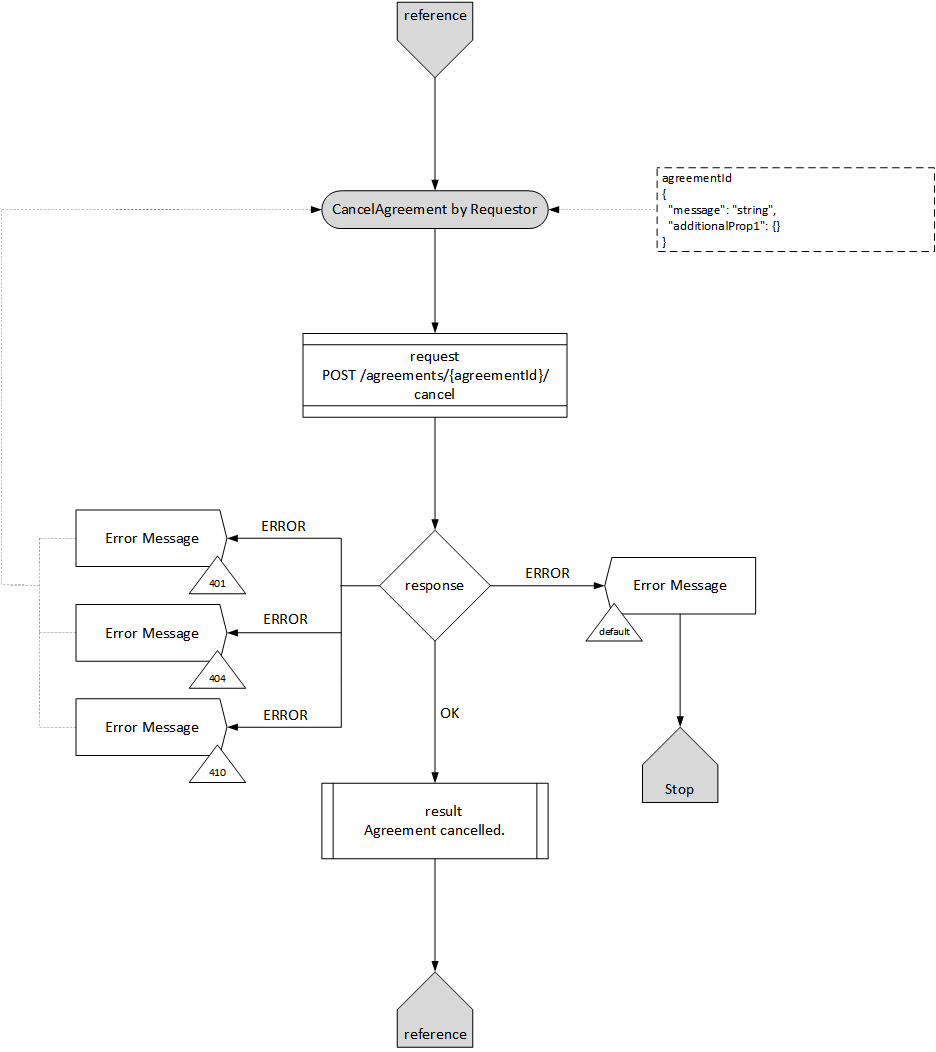
\includegraphics[width=11cm,height=11cm,angle=0]{./diag/Workflow/Market/CancelAgreement-R-Workflow.png}
    \caption{Requestor Workflow Cancel Agreement  }
	\label{fig:RCCA}
\end{figure}

\end{enumerate}

\newpage

% WaitAgreement WaitForApproval

\subsubsubsubsection{WaitForApproval Function}

\begin{enumerate}

\item Profile

\begin{enumerate}

\item Description

The WaitForApproval function is used to wait for Agreement approval by the Provider. This method is used by the Requestor node. 
It uses the POST /agreements/\{agreementId\}/wait method.

\item Side

Requestor

\end{enumerate}

\item Request

\begin{enumerate}

\item Input

\begin{tcolorbox}[boxrule=0pt, frame empty]
\begin{verbatim}

agreementId
timeout

\end{verbatim}
\end{tcolorbox}

%Object
%\begin{tcolorbox}[boxrule=0pt, frame empty]
%\begin{verbatim}
%{
%  "message": "string",
%  "additionalProp1": {}
%}
%\end{verbatim}
%\end{tcolorbox}

\begin{center}
\begin{tabular}{|p{3cm}|l|p{3cm}|p{3cm}|p{4cm}|} 
\hline
\rowcolor{lightgray}	Name	& MO.	& Type	& Example & 	Description \\
\hline

agreementId		& M & 	string				&		& 	Agreement Identifier \\
\hline

timeout 		& O	& 	number(\$float)				&	5	&	Timeout used in blocking calls waiting for eg. acknowledgement. 
																How many seconds server should wait for response/acknowledgement of an action 
																(0.0 means it should wait for other party's response indefinitely)	\\ 
\hline

\end{tabular}
\end{center}

\item REST Method

\begin{tcolorbox}[boxrule=0pt, frame empty]
\begin{verbatim} 

POST /agreements/{agreementId}/wait

\end{verbatim}
\end{tcolorbox}

\end{enumerate}

\item Response

\begin{center}
\begin{tabular}{|c|l|} 
\hline
\rowcolor{lightgray}	Code 		& 	Description \\
\hline
204	 		&	Agreement approved by the Provider. \\
\hline
404			&	(404) The specified resource was not found. \\
\hline
401			&	(401) Authorization information is missing or invalid. \\
\hline
408			&	(408) Timeout. \\
\hline
409			&	(409) Conflict. \\
\hline
410			&	(410) Gone \\
\hline
default		&	Unexpected error. \\
\hline
\end{tabular}
\end{center}

\item Result

\begin{tcolorbox}[boxrule=0pt, frame empty]
\begin{verbatim}

None

\end{verbatim}
\end{tcolorbox}

%\begin{center}
%\begin{tabular}{|p{3cm}|l|p{3cm}|p{3cm}|p{4cm}|} 
%\hline
%\rowcolor{lightgray}	Name	& MO.	& Type	& Example & 	Description \\
%\hline
%agreementId		& 	& 	string				&						&	Agreement Identyfier \\ 
%\hline
%eventDate		& 	& 	string(\$date-time)	&	YYYY-MM-DDThh:mm:ss.sssZ	&	 \\ 
%\hline
%eventType		& 	& 	string(enum)		&	 &	Event Type \\ 
%\hline
%\end{tabular}
%\end{center}

\item Workflow

(Please see Figure ~\ref{fig:RWW} on page ~\pageref{fig:RWW}):

\begin{figure}[htbp]
    \centering
    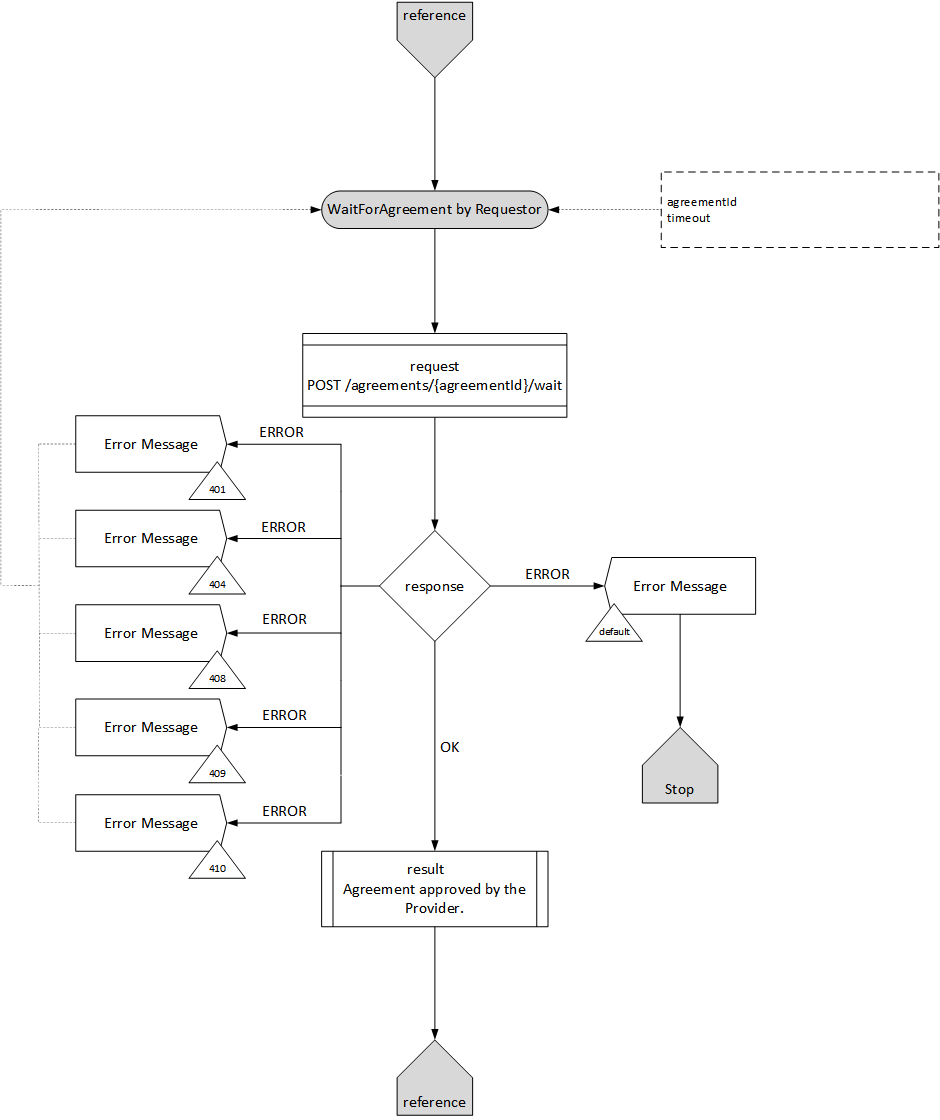
\includegraphics[width=11cm,height=11cm,angle=0]{./diag/Workflow/Market/WaitForAgreement-R-Workflow.png}
    \caption{Requestor Workflow WaitForApproval }
	\label{fig:RWW}
\end{figure}

\end{enumerate}

\newpage

% ApproveAgreement

\subsubsubsubsection{ApproveAgreement Function}

\begin{enumerate}

\item Profile

\begin{enumerate}

\item Description

The ApproveAgreement function is used to approve Agreement proposed by Requestor. This method is used by the Provider node. 
It uses the POST /agreements/\{agreementId\}/approve method.

\item Side

Provider

\end{enumerate}

\item Request

\begin{enumerate}

\item Input

\begin{tcolorbox}[boxrule=0pt, frame empty]
\begin{verbatim}

agreementId
appSessionId
timeout

\end{verbatim}
\end{tcolorbox}

%Object
%\begin{tcolorbox}[boxrule=0pt, frame empty]
%\begin{verbatim}
%{
%  "message": "string",
%  "additionalProp1": {}
%}
%\end{verbatim}
%\end{tcolorbox}

\begin{center}
\begin{tabular}{|p{3cm}|l|p{3cm}|p{3cm}|p{4cm}|} 
\hline
\rowcolor{lightgray}	Name	& MO.	& Type	& Example & 	Description \\
\hline

agreementId		& M & 	string				&		& 	Agreement Identifier \\
\hline

appSessionId	& O	& 	string				&		&	A correlation/session identifier used for querying events related to an action where this appSessionId has been specified 	\\ 
\hline

timeout			& O & 	number(\$float)		&	5 	&  Timeout used in blocking calls waiting for eg. acknowledgement. 
														How many seconds server should wait for response/acknowledgement of an action 
														(0.0 means it should wait for other party's response indefinitely) \\
\hline
\end{tabular}
\end{center}

\item REST Method

\begin{tcolorbox}[boxrule=0pt, frame empty]
\begin{verbatim} 

POST /agreements/{agreementId}/approve

\end{verbatim}
\end{tcolorbox}

\end{enumerate}

\item Response

\begin{center}
\begin{tabular}{|c|l|} 
\hline
\rowcolor{lightgray}	Code 		& 	Description \\
\hline
204	 		&	Agreement approved. \\
\hline
404			&	(404) The specified resource was not found. \\
\hline
401			&	(401) Authorization information is missing or invalid. \\
\hline
408			&	(408) Timeout. \\
\hline
410			&	(410) Gone \\
\hline
default		&	Unexpected error. \\
\hline
\end{tabular}
\end{center}

\item Result

\begin{tcolorbox}[boxrule=0pt, frame empty]
\begin{verbatim}

None

\end{verbatim}
\end{tcolorbox}

%\begin{center}
%\begin{tabular}{|p{3cm}|l|p{3cm}|p{3cm}|p{4cm}|} 
%\hline
%\rowcolor{lightgray}	Name	& MO.	& Type	& Example & 	Description \\
%\hline
%agreementId		& 	& 	string				&						&	Agreement Identyfier \\ 
%\hline
%eventDate		& 	& 	string(\$date-time)	&	YYYY-MM-DDThh:mm:ss.sssZ	&	 \\ 
%\hline
%eventType		& 	& 	string(enum)		&	 &	Event Type \\ 
%\hline
%\end{tabular}
%\end{center}

\item Workflow

(Please see Figure ~\ref{fig:PAA} on page ~\pageref{fig:PAA}):

\begin{figure}[htbp]
    \centering
    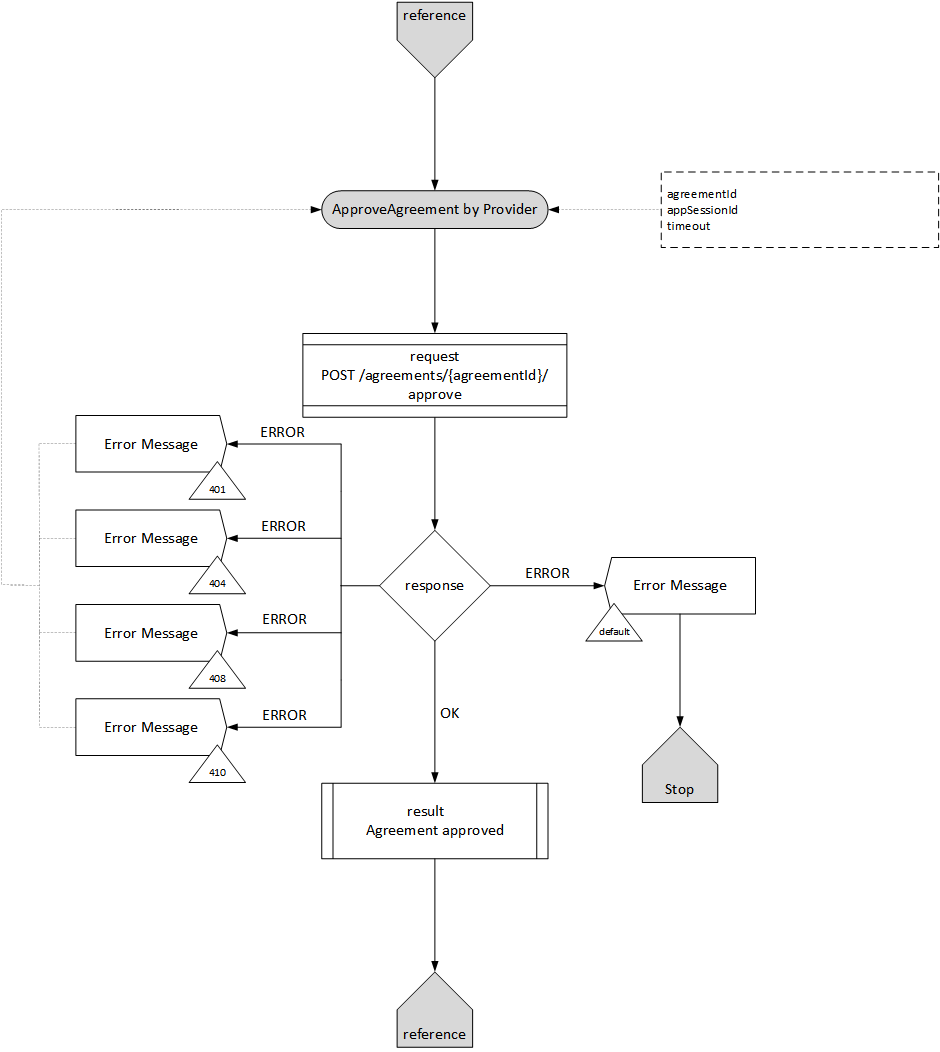
\includegraphics[width=11cm,height=11cm,angle=0]{./diag/Workflow/Market/ApproveAgreement-P-Workflow.png}
    \caption{Provider Workflow Approve Agreement  }
	\label{fig:PAA}
\end{figure}

\end{enumerate}

\newpage

% RejectAgreement

\subsubsubsubsection{RejectAgreement Function}

\begin{enumerate}

\item Profile

\begin{enumerate}

\item Description

The RejectAgreement function is used to reject Agreement object proposed by Requestor. This method is used by the Provider node. 
It uses the POST /agreements/\{agreementId\}/reject method.

\item Side

Provider

\end{enumerate}

\item Request

\begin{enumerate}

\item Input

\begin{tcolorbox}[boxrule=0pt, frame empty]
\begin{verbatim}

agreementId

\end{verbatim}
\end{tcolorbox}

Object
\begin{tcolorbox}[boxrule=0pt, frame empty]
\begin{verbatim}
{
  "message": "string",
  "additionalProp1": {}
}
\end{verbatim}
\end{tcolorbox}

\begin{center}
\begin{tabular}{|p{3cm}|l|p{3cm}|p{3cm}|p{4cm}|} 
\hline
\rowcolor{lightgray}	Name	& MO.	& Type	& Example & 	Description \\
\hline

agreementId		& M & 	string				&		& 	Agreement Identifier \\
\hline

message 		& O	& 	string				&		&	 	\\ 
\hline

additionalProp1 & O	& 	json				&		&	 	\\ 
\hline

\end{tabular}
\end{center}

\item REST Method

\begin{tcolorbox}[boxrule=0pt, frame empty]
\begin{verbatim} 

POST /agreements/{agreementId}/reject

\end{verbatim}
\end{tcolorbox}

\end{enumerate}

\item Response

\begin{center}
\begin{tabular}{|c|l|} 
\hline
\rowcolor{lightgray}	Code 		& 	Description \\
\hline
204	 		&	Agreement rejected. \\
\hline
404			&	(404) The specified resource was not found. \\
\hline
401			&	(401) Authorization information is missing or invalid. \\
\hline
410			&	(410) Gone \\
\hline
default		&	Unexpected error. \\
\hline
\end{tabular}
\end{center}

\item Result

\begin{tcolorbox}[boxrule=0pt, frame empty]
\begin{verbatim}

None

\end{verbatim}
\end{tcolorbox}

%\begin{center}
%\begin{tabular}{|p{3cm}|l|p{3cm}|p{3cm}|p{4cm}|} 
%\hline
%\rowcolor{lightgray}	Name	& MO.	& Type	& Example & 	Description \\
%\hline
%agreementId		& 	& 	string				&						&	Agreement Identyfier \\ 
%\hline
%eventDate		& 	& 	string(\$date-time)	&	YYYY-MM-DDThh:mm:ss.sssZ	&	 \\ 
%\hline
%eventType		& 	& 	string(enum)		&	 &	Event Type \\ 
%\hline
%\end{tabular}
%\end{center}

\item Workflow

(Please see Figure ~\ref{fig:PRA} on page ~\pageref{fig:PRA}):

\begin{figure}[htbp]
    \centering
    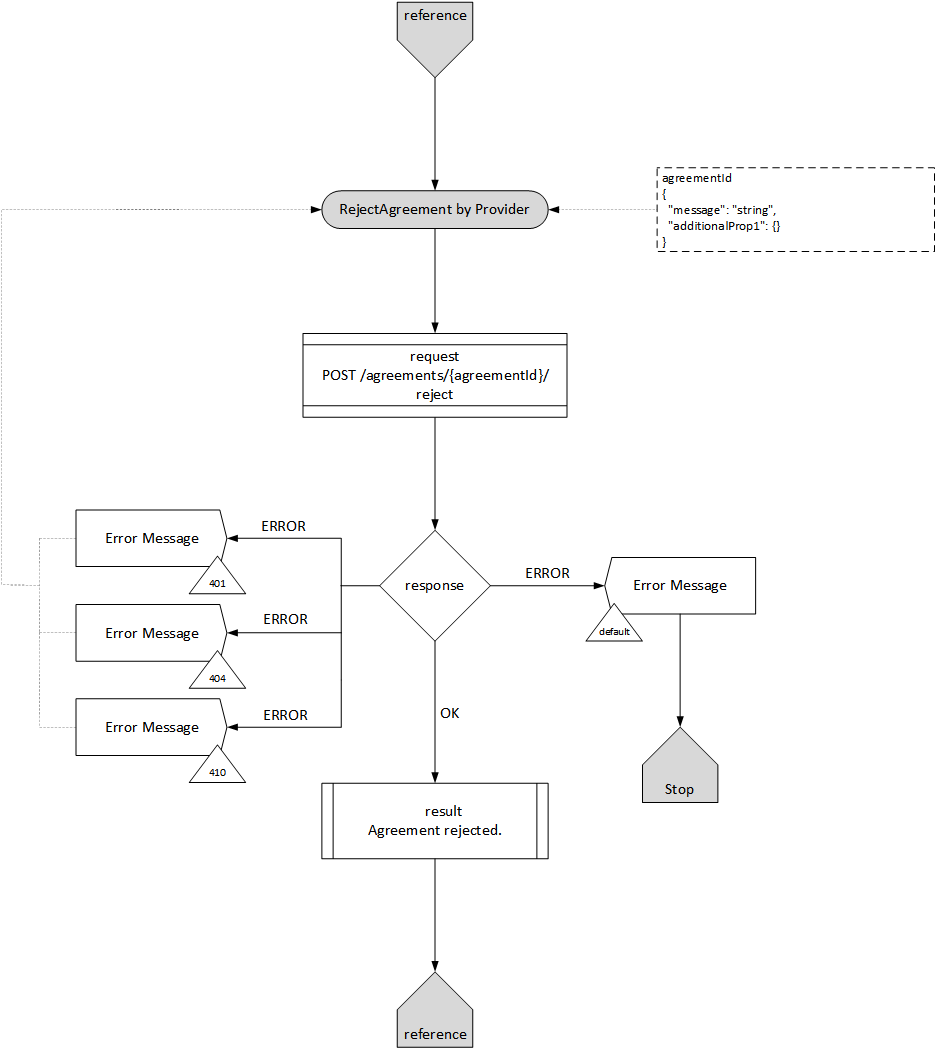
\includegraphics[width=11cm,height=11cm,angle=0]{./diag/Workflow/Market/RejectAgreement-P-Workflow.png}
    \caption{Provider Workflow Reject Agreement  }
	\label{fig:PRA}
\end{figure}

\end{enumerate}

\newpage



\subsubsubsection{Golem Activity Service API}

\subsubsubsection{Golem Payment Service API}

\newpage

\subsubsubsection{IssueDebitNote Function}

\begin{enumerate}

\item Profile

\begin{enumerate}

\item Description

The IssueDebitNote function is used to create the DebitNote Object by the Provider Node. It uses the POST /debitNotes method.
The DebitNote object is used for short-term billing of computing resource usage between a Provider node and a Requestor node.
 
\item Side

Provider

\end{enumerate}

\item Request

\begin{enumerate}

\item Input

\begin{tcolorbox}[boxrule=0pt, frame empty]
\begin{verbatim}

No parameters

\end{verbatim}
\end{tcolorbox}

Object

\begin{tcolorbox}[boxrule=0pt, frame empty]
\begin{verbatim}

{
  "activityId": "string",
  "totalAmountDue": "string",
  "usageCounterVector": {},
  "paymentDueDate": "YYYY-MM-DDThh:mm:ss.sssZ"
}

\end{verbatim}
\end{tcolorbox}

\begin{table}[H]
\footnotesize

\begin{center}
\begin{tabular}{|p{3cm}|l|p{3cm}|p{3cm}|p{4cm}|} 
\hline
\rowcolor{lightgray}	Name	& MO.	& Type	& Example & 	Description \\
\hline

activityId				& M	& 	string				&								&	Activity Identifier \\ 
\hline

totalAmountDue			& M	& 	string				&								&	Total Amount Due \\ 
\hline

usageCounterVector		& M & 	json				&								&	Usage Counter Vector \\
\hline

paymentDueDate			& M &	string(\$date-time)	&	YYYY-MM-DDThh:mm:ss.sssZ	&	Payment Due Date \\
\hline

\end{tabular}
\end{center}
\end{table}


\item REST Method

\begin{tcolorbox}[boxrule=0pt, frame empty]
\begin{verbatim} 

POST /debitNotes

\end{verbatim}
\end{tcolorbox}

\end{enumerate}

\item Response

\begin{table}[H]
\footnotesize

\begin{center}
\begin{tabular}{|c|l|} 
\hline
\rowcolor{lightgray}	Code 		& 	Description \\
\hline
201	 		&	OK \\
\hline
400			&	(400) Bad request \\
\hline
401			&	(401) Authorization information is missing or invalid. \\
\hline
500			&	(500) Server error. \\
\hline
\end{tabular}
\end{center}
\end{table}

\item Result

\begin{tcolorbox}[boxrule=0pt, frame empty]
\begin{verbatim}

{
  "debitNoteId": "string",
  "issuerId": "string",
  "recipientId": "string",
  "payeeAddr": "string",
  "payerAddr": "string",
  "paymentPlatform": "string",
  "previousDebitNoteId": "string",
  "timestamp": "YYYY-MM-DDThh:mm:ss.sss",
  "agreementId": "string",
  "activityId": "string",
  "totalAmountDue": "string",
  "usageCounterVector": {},
  "paymentDueDate": "YYYY-MM-DDThh:mm:ss.sssZ",
  "status": "ISSUED"
}

\end{verbatim}
\end{tcolorbox}

\begin{table}[H]
\footnotesize

\begin{center}
\begin{tabular}{|p{3cm}|l|p{3cm}|p{3cm}|p{4cm}|} 
\hline
\rowcolor{lightgray}	Name	& MO.	& Type	& Example & 	Description \\
\hline

debitNoteId				&	&	string				&																		&	Debit Note Identifier \\
\hline   

issuerId				&	&	string				&																		&	Issuer Identifier \\
\hline   
  
recipientId				&	&	string				&																		&	Recipient Identifier \\
\hline   

payeeAddr				&	&	string				&																		&	Payee Address \\
\hline   
  
payerAddr				&	&	string				&																		&	Payer Address \\
\hline
   
paymentPlatform			&	&	object(string)		&																		&	Payment Platform Object \\
\hline

previousDebitNoteId		&	&	string				&																		& 	Last Debit Note Id \\
\hline

timestamp				&   &	string(\$date-time)	&	YYYY-MM-DDThh:mm:ss.sssZ											&	Time of ? \\
\hline

agreementId				& 	& 	string				&																		&	Agreement Identifier \\ 
\hline

activityId				& 	& 	string				&																		&	Activity Identifier \\ 
\hline

totalAmountDue			& 	& 	string				&																		&	Total Amount Due \\ 
\hline

usageCounterVector		&   & 	json				&																		&	Usage Counter Vector \\
\hline

paymentDueDate			&   &	string(\$date-time)	&	YYYY-MM-DDThh:mm:ss.sssZ											&	Payment Due Date \\
\hline

status					&	&	string(enum)		&	[ISSUED, RECEIVED, ACCEPTED, REJECTED, FAILED, SETTLED, CANCELLED]	& 	Debit Note state \\	
\hline

\end{tabular}
\end{center}
\end{table}

\item Workflow

(Please see Figure ~\ref{fig:PCDN} on page ~\pageref{fig:PCDN}):

\begin{figure}[htbp]
    \centering
    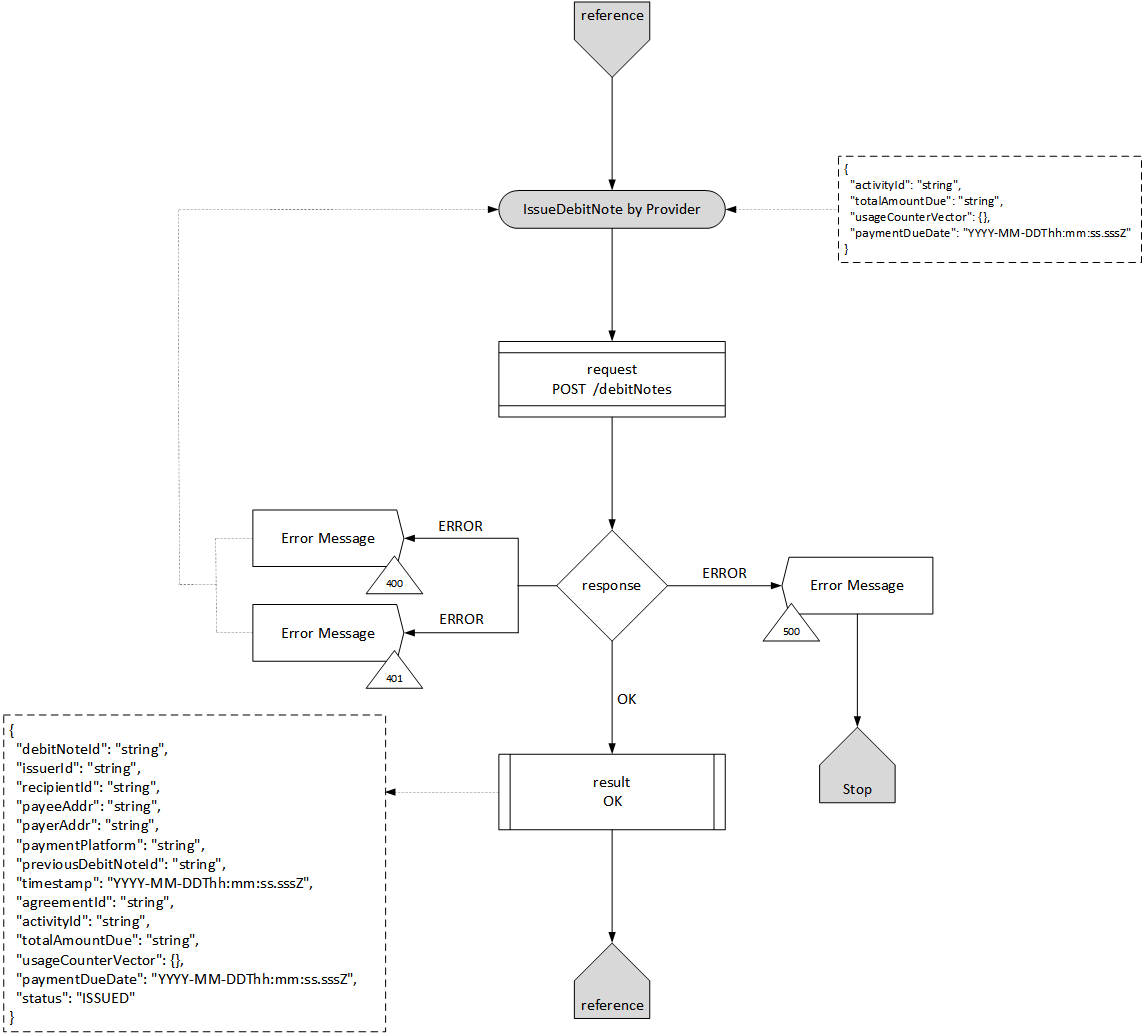
\includegraphics[width=12cm,height=12cm,angle=0]{./diag/Workflow/Payment/IssueDebitNote-P-Workflow.png}
    \caption{Provider Workflow Create Debit Note }
	\label{fig:PCDN}
\end{figure}


\end{enumerate}

\newpage

%% List Debit Notes

\subsubsubsection{ListDebitNotes Function}

\begin{enumerate}

\item Profile

\begin{enumerate}

\item Description

The ListDebitNotes function is used to get the DebitNote Objects by the Provider Node and Requestor Node. 
It uses the GET /debitNotes method.
 
\item Side

Both

\end{enumerate}

\item Request

\begin{enumerate}

\item Input

\begin{tcolorbox}[boxrule=0pt, frame empty]
\begin{verbatim}

afterTimestamp
maxItems

\end{verbatim}
\end{tcolorbox}

%Object
%\begin{tcolorbox}[boxrule=0pt, frame empty]
%\begin{verbatim}
%{
%  "activityId": "string",
%  "totalAmountDue": "string",
%  "usageCounterVector": {},
%  "paymentDueDate": "YYYY-MM-DDThh:mm:ss.sssZ"
%}
%\end{verbatim}
%\end{tcolorbox}

\begin{table}[H]
\footnotesize

\begin{center}
\begin{tabular}{|p{3cm}|l|p{3cm}|p{3cm}|p{4cm}|} 
\hline
\rowcolor{lightgray}	Name	& MO.	& Type	& Example & 	Description \\
\hline

maxItems				& O	& 	integer(\$int32)	&	10							&	Maximum number of items that server should return at once. \\ 
\hline

afterTimestamp			& O &	string(\$date-time)	&	YYYY-MM-DDThh:mm:ss.sssZ	&	Apply only to records created later than the specified timestamp \\
\hline

\end{tabular}
\end{center}
\end{table}


\item REST Method

\begin{tcolorbox}[boxrule=0pt, frame empty]
\begin{verbatim} 

GET /debitNotes

\end{verbatim}
\end{tcolorbox}

\end{enumerate}

\item Response

\begin{table}[H]
\footnotesize
\begin{center}
\begin{tabular}{|c|l|} 
\hline
\rowcolor{lightgray}	Code 		& 	Description \\
\hline
201	 		&	OK \\
\hline
401			&	(401) Authorization information is missing or invalid. \\
\hline
500			&	(500) Server error. \\
\hline
\end{tabular}
\end{center}
\end{table}

\item Result

\begin{tcolorbox}[boxrule=0pt, frame empty]
\begin{verbatim}

[
	{
		"debitNoteId": "string",
		"issuerId": "string",
		"recipientId": "string",
		"payeeAddr": "string",
		"payerAddr": "string",
		"paymentPlatform": "string",
		"previousDebitNoteId": "string",
		"timestamp": "YYYY-MM-DDThh:mm:ss.sss",
		"agreementId": "string",
		"activityId": "string",
		"totalAmountDue": "string",
		"usageCounterVector": {},
		"paymentDueDate": "YYYY-MM-DDThh:mm:ss.sssZ",
		"status": "ISSUED"
	}
]

\end{verbatim}
\end{tcolorbox}

\begin{table}[H]
\footnotesize

\begin{center}
\begin{tabular}{|p{3cm}|l|p{3cm}|p{3cm}|p{4cm}|} 
\hline
\rowcolor{lightgray}	Name	& MO.	& Type	& Example & 	Description \\
\hline

debitNoteId				&	&	string				&																		&	Debit Note Identifier \\
\hline   

issuerId				&	&	string				&																		&	Issuer Identifier \\
\hline   
  
recipientId				&	&	string				&																		&	Recipient Identifier \\
\hline   

payeeAddr				&	&	string				&																		&	Payee Address \\
\hline   
  
payerAddr				&	&	string				&																		&	Payer Address \\
\hline
   
paymentPlatform			&	&	object(string)		&																		&	Payment Platform Object \\
\hline

previousDebitNoteId		&	&	string				&																		& 	Last Debit Note Id \\
\hline

timestamp				&   &	string(\$date-time)	&	YYYY-MM-DDThh:mm:ss.sssZ											&	Time of ? \\
\hline

agreementId				& 	& 	string				&																		&	Agreement Identifier \\ 
\hline

activityId				& 	& 	string				&																		&	Activity Identifier \\ 
\hline

totalAmountDue			& 	& 	string				&																		&	Total Amount Due \\ 
\hline

usageCounterVector		&   & 	json				&																		&	Usage Counter Vector \\
\hline

paymentDueDate			&   &	string(\$date-time)	&	YYYY-MM-DDThh:mm:ss.sssZ											&	Payment Due Date \\
\hline

status					&	&	string(enum)		&	[ISSUED, RECEIVED, ACCEPTED, REJECTED, FAILED, SETTLED, CANCELLED]	& 	Debit Note state \\	
\hline

\end{tabular}
\end{center}
\end{table}

\item Workflow

(Please see Figure ~\ref{fig:BLDN} on page ~\pageref{fig:BLDN}):

\begin{figure}[htbp]
    \centering
    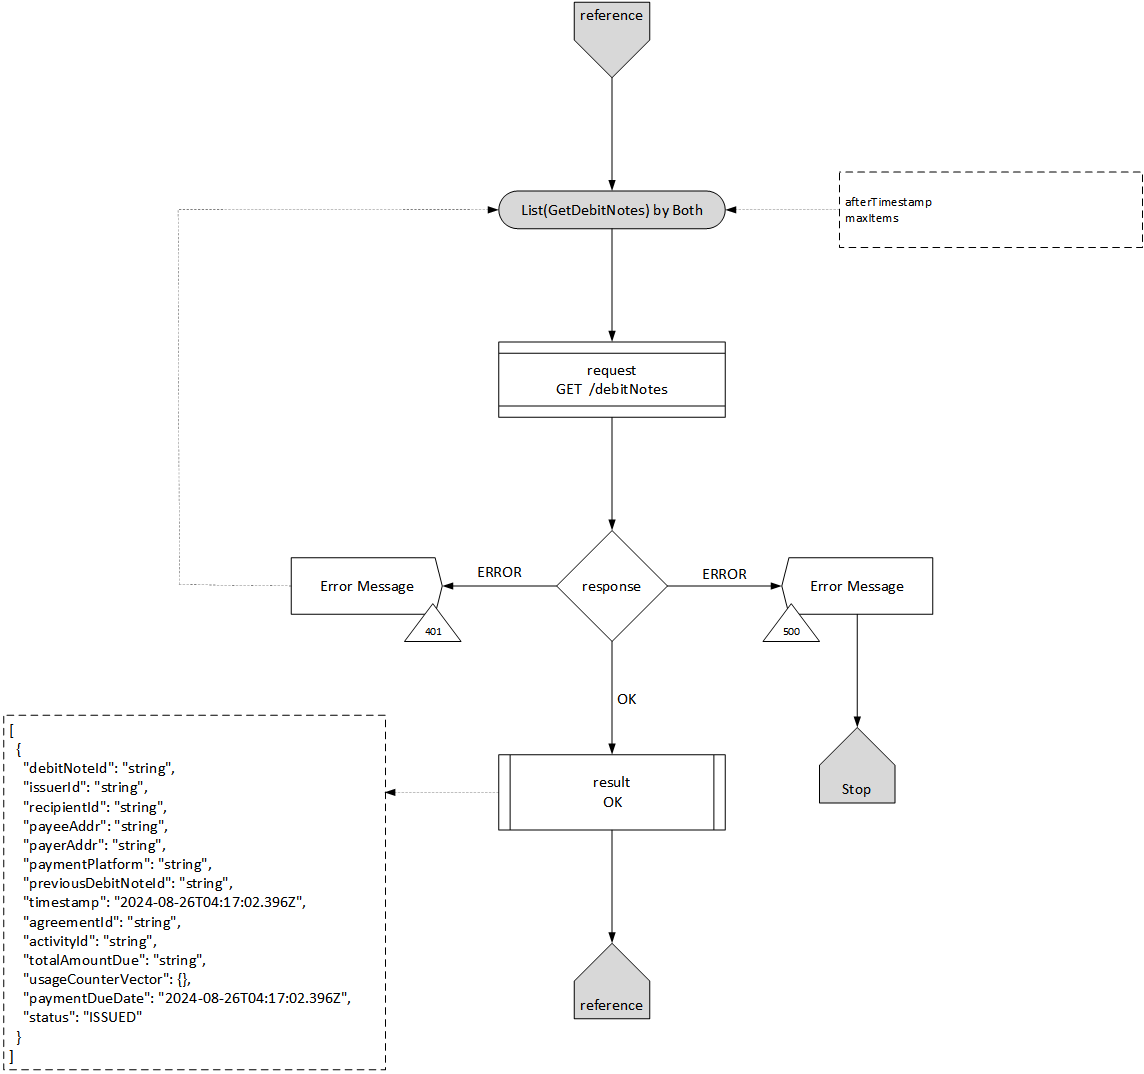
\includegraphics[width=12cm,height=12cm,angle=0]{./diag/Workflow/Payment/List(GetDebitNotes)-B-Workflow.png}
    \caption{Both Workflow List Debit Notes }
	\label{fig:BLDN}
\end{figure}


\end{enumerate}

\newpage

%% Get Debit Notes

\subsubsubsection{GetDebitNote Function}

\begin{enumerate}

\item Profile

\begin{enumerate}

\item Description

The GetDebitNote function is used to get the DebitNote Object by the Provider Node and Requestor Node. 
It uses the GET /debitNotes/\{debitNoteId\} method.
 
\item Side

Both

\end{enumerate}

\item Request

\begin{enumerate}

\item Input

\begin{tcolorbox}[boxrule=0pt, frame empty]
\begin{verbatim}

debitNoteId

\end{verbatim}
\end{tcolorbox}

%Object
%\begin{tcolorbox}[boxrule=0pt, frame empty]
%\begin{verbatim}
%{
%  "activityId": "string",
%  "totalAmountDue": "string",
%  "usageCounterVector": {},
%  "paymentDueDate": "YYYY-MM-DDThh:mm:ss.sssZ"
%}
%\end{verbatim}
%\end{tcolorbox}

\begin{table}[H]
\footnotesize

\begin{center}
\begin{tabular}{|p{3cm}|l|p{3cm}|p{3cm}|p{4cm}|} 
\hline
\rowcolor{lightgray}	Name	& MO.	& Type	& Example & 	Description \\
\hline

debitNoteId				& M	& 	string				&								&	Debit Note Identifier \\ 
\hline

%afterTimestamp			& O &	string(\$date-time)	&	YYYY-MM-DDThh:mm:ss.sssZ	&	Apply only to records created later than the specified timestamp \\
%\hline

\end{tabular}
\end{center}
\end{table}


\item REST Method

\begin{tcolorbox}[boxrule=0pt, frame empty]
\begin{verbatim} 

GET /debitNotes/{debitNoteId}

\end{verbatim}
\end{tcolorbox}

\end{enumerate}

\item Response

\begin{table}[H]
\footnotesize

\begin{center}
\begin{tabular}{|c|l|} 
\hline
\rowcolor{lightgray}	Code 		& 	Description \\
\hline
201	 		&	OK \\
\hline
401			&	(401) Authorization information is missing or invalid. \\
\hline
404			&	(404) The specified resource was not found \\
\hline
500			&	(500) Server error. \\
\hline
\end{tabular}
\end{center}

\end{table}

\item Result

\begin{tcolorbox}[boxrule=0pt, frame empty]
\begin{verbatim}


{
	"debitNoteId": "string",
	"issuerId": "string",
	"recipientId": "string",
	"payeeAddr": "string",
	"payerAddr": "string",
	"paymentPlatform": "string",
	"previousDebitNoteId": "string",
	"timestamp": "YYYY-MM-DDThh:mm:ss.sss",
	"agreementId": "string",
	"activityId": "string",
	"totalAmountDue": "string",
	"usageCounterVector": {},
	"paymentDueDate": "YYYY-MM-DDThh:mm:ss.sssZ",
	"status": "ISSUED"
}


\end{verbatim}
\end{tcolorbox}

\begin{table}
\footnotesize

\begin{center}
\begin{tabular}{|p{3cm}|l|p{3cm}|p{3cm}|p{4cm}|} 
\hline
\rowcolor{lightgray}	Name	& MO.	& Type	& Example & 	Description \\
\hline

debitNoteId				&	&	string				&																		&	Debit Note Identifier \\
\hline   

issuerId				&	&	string				&																		&	Issuer Identifier \\
\hline   
  
recipientId				&	&	string				&																		&	Recipient Identifier \\
\hline   

payeeAddr				&	&	string				&																		&	Payee Address \\
\hline   
  
payerAddr				&	&	string				&																		&	Payer Address \\
\hline
   
paymentPlatform			&	&	object(string)		&																		&	Payment Platform Object \\
\hline

previousDebitNoteId		&	&	string				&																		& 	Last Debit Note Id \\
\hline

timestamp				&   &	string(\$date-time)	&	YYYY-MM-DDThh:mm:ss.sssZ											&	Time of ? \\
\hline

agreementId				& 	& 	string				&																		&	Agreement Identifier \\ 
\hline

activityId				& 	& 	string				&																		&	Activity Identifier \\ 
\hline

totalAmountDue			& 	& 	string				&																		&	Total Amount Due \\ 
\hline

usageCounterVector		&   & 	json				&																		&	Usage Counter Vector \\
\hline

paymentDueDate			&   &	string(\$date-time)	&	YYYY-MM-DDThh:mm:ss.sssZ											&	Payment Due Date \\
\hline

status					&	&	string(enum)		&	[ISSUED, RECEIVED, ACCEPTED, REJECTED, FAILED, SETTLED, CANCELLED]	& 	Debit Note state \\	
\hline

\end{tabular}
\end{center}
\end{table}

\item Workflow

(Please see Figure ~\ref{fig:BGDN} on page ~\pageref{fig:BGDN}):

\begin{figure}[htbp]
    \centering
    \includegraphics[width=12cm,height=12cm,angle=0]{./diag/Workflow/Payment/GetDebitNote-B-Workflow.png}
    \caption{Both Workflow Get Debit Note }
	\label{fig:BGDN}
\end{figure}


\end{enumerate}

\newpage

%% DebitNoteEvents

\subsubsubsection{CollectDebitNoteInvoiceEvent Function}

\begin{enumerate}

\item Profile

\begin{enumerate}

\item Description

The CollectDebitNoteInvoiceEvent function is used to get the DebitNote events by the Provider Node and Requestor Node. 
It uses the GET /debitNoteEvents method.
 
\item Side

Both

\end{enumerate}

\item Request

\begin{enumerate}

\item Input

\begin{tcolorbox}[boxrule=0pt, frame empty]
\begin{verbatim}

timeout
afterTimestamp
maxEvents
appSessionId

\end{verbatim}
\end{tcolorbox}

%Object
%\begin{tcolorbox}[boxrule=0pt, frame empty]
%\begin{verbatim}
%{
%  "activityId": "string",
%  "totalAmountDue": "string",
%  "usageCounterVector": {},
%  "paymentDueDate": "YYYY-MM-DDThh:mm:ss.sssZ"
%}
%\end{verbatim}
%\end{tcolorbox}

\begin{table}[H]
\footnotesize

\begin{center}
\begin{tabular}{|p{3cm}|l|p{3cm}|p{3cm}|p{4cm}|} 
\hline
\rowcolor{lightgray}	Name	& MO.	& Type	& Example & 	Description \\
\hline

timeout					& O	& 	number(\$float)		&	5							&	Timeout used in long-polling calls (in seconds). 
																						How many seconds server should wait for response containing new events 
																						(0.0 means it should return immediately if there are no events) \\ 
\hline

afterTimestamp			& O &	string(\$date-time)	&	YYYY-MM-DDThh:mm:ss.sssZ	&	Apply only to records created later than the specified timestamp \\
\hline

maxEvents				& O & 	integer(\$int32)	&	10							&	Maximum number of events that server should return at once. \\
\hline

appSessionId			& O &	string				&								&	A correlation/session identifier used for querying events related to 
																						an action where this appSessionId has been specified \\
\hline

\end{tabular}
\end{center}
\end{table}


\item REST Method

\begin{tcolorbox}[boxrule=0pt, frame empty]
\begin{verbatim} 

GET /debitNoteEvents

\end{verbatim}
\end{tcolorbox}

\end{enumerate}

\item Response

\begin{table}[H]
\footnotesize

\begin{center}
\begin{tabular}{|c|l|} 
\hline
\rowcolor{lightgray}	Code 		& 	Description \\
\hline
201	 		&	OK \\
\hline
401			&	(401) Authorization information is missing or invalid. \\
\hline
%404			&	(404) The specified resource was not found \\
%\hline
500			&	(500) Server error. \\
\hline
\end{tabular}
\end{center}

\end{table}

\item Result

\begin{tcolorbox}[boxrule=0pt, frame empty]
\begin{verbatim}

[
  {
    "eventType": "string",
    "eventDate": "YYYY-MM-DDThh:mm:ss.sssZ",
    "debitNoteId": "string"
  }
]


\end{verbatim}
\end{tcolorbox}

\begin{table}[H]
\footnotesize

\begin{center}
\begin{tabular}{|p{3cm}|l|p{3cm}|p{3cm}|p{4cm}|} 
\hline
\rowcolor{lightgray}	Name	& MO.	& Type	& Example & 	Description \\
\hline

debitNoteId				&	&	string				&																		&	Debit Note Identifier \\
\hline   

eventDate				&   &	string(\$date-time)	&	YYYY-MM-DDThh:mm:ss.sssZ											&	Event Date \\
\hline

eventType				&	&	string				&																		& 	Event Type \\	
\hline

\end{tabular}
\end{center}
\end{table}

\item Workflow

(Please see Figure ~\ref{fig:BGDNE} on page ~\pageref{fig:BGDNE}):

\begin{figure}[htbp]
    \centering
    \includegraphics[width=12cm,height=12cm,angle=0]{./diag/Workflow/Payment/DebitNoteEvents-B-Workflow.png}
    \caption{Both Workflow Get Debit Note Events }
	\label{fig:BGDNE}
\end{figure}


\end{enumerate}

\newpage

% SendDebitNote 

\subsubsubsection{SendDebitNote Function}

\begin{enumerate}

\item Profile

\begin{enumerate}

\item Description

The SendDebitNote function is used to send the DebitNote Object from the Provider Node to the Requestor Node. 
It uses the POST /debitNotes/\{debitNoteId\}/send method.

\item Side

Provider

\end{enumerate}

\item Request

\begin{enumerate}

\item Input

\begin{tcolorbox}[boxrule=0pt, frame empty]
\begin{verbatim}

debitNoteId
timeout

\end{verbatim}
\end{tcolorbox}

%Object

%\begin{tcolorbox}[boxrule=0pt, frame empty]
%\begin{verbatim}

%{
%  "activityId": "string",
%  "totalAmountDue": "string",
%  "usageCounterVector": {},
%  "paymentDueDate": "YYYY-MM-DDThh:mm:ss.sssZ"
%}

%\end{verbatim}
%\end{tcolorbox}

\begin{table}[H]
\footnotesize

\begin{center}
\begin{tabular}{|p{3cm}|l|p{3cm}|p{3cm}|p{4cm}|} 
\hline
\rowcolor{lightgray}	Name	& MO.	& Type	& Example & 	Description \\
\hline

debitNoteId				& M	&	string				&								&	Debit Note Identifier \\
\hline   

timeout					& O &	number(\$float)		&	5							&	Timeout used in blocking calls waiting for eg. acknowledgement. 
																						How many seconds server should wait for response/acknowledgement 
																						of an action 
																						(0.0 means it should wait for other party's response indefinitely) \\
\hline

\end{tabular}
\end{center}
\end{table}


\item REST Method

\begin{tcolorbox}[boxrule=0pt, frame empty]
\begin{verbatim} 

POST /debitNotes/{debitNoteId}/send

\end{verbatim}
\end{tcolorbox}

\end{enumerate}

\item Response

\begin{table}[H]
\footnotesize

\begin{center}
\begin{tabular}{|c|l|} 
\hline
\rowcolor{lightgray}	Code 		& 	Description \\
\hline
200	 		&	OK \\
\hline
404			&	(404) The specified resource was not found. \\
\hline
401			&	(401) Authorization information is missing or invalid. \\
\hline
500			&	(500) Server error. \\
\hline
504			&	(504) Ack timeout. \\
\hline

\end{tabular}
\end{center}

\end{table}

\item Result

\begin{tcolorbox}[boxrule=0pt, frame empty]
\begin{verbatim}

As above

\end{verbatim}
\end{tcolorbox}

%\begin{table}[H]
%\footnotesize
%\begin{center}
%\begin{tabular}{|p{3cm}|l|p{3cm}|p{3cm}|p{4cm}|} 
%\hline
%\rowcolor{lightgray}	Name	& MO.	& Type	& Example & 	Description \\
%\hline	
%\end{tabular}
%\end{center}
%\end{table}

\item Workflow

(Please see Figure ~\ref{fig:PSDN} on page ~\pageref{fig:PSDN}):

\begin{figure}[htbp]
    \centering
    \includegraphics[width=12cm,height=12cm,angle=0]{./diag/Workflow/Payment/SendDebitNote-P-Workflow.png}
    \caption{Provider Workflow Send Debit Note }
	\label{fig:PSDN}
\end{figure}


\end{enumerate}

\newpage


% AcceptDebitNote 

\subsubsubsection{AcceptDebitNote Function}

\begin{enumerate}

\item Profile

\begin{enumerate}

\item Description

The AcceptDebitNote function is used to accept received the DebitNote Object by the Requestor Node. 
It uses the POST /debitNotes/\{debitNoteId\}/accept method.

\item Side

Requestor

\end{enumerate}

\item Request

\begin{enumerate}

\item Input

\begin{tcolorbox}[boxrule=0pt, frame empty]
\begin{verbatim}

debitNoteId
timeout

\end{verbatim}
\end{tcolorbox}

Object

\begin{tcolorbox}[boxrule=0pt, frame empty]
\begin{verbatim}

{
  "totalAmountAccepted": "string",
  "allocationId": "string",
  "autoAcceptTo": "string"
}

\end{verbatim}
\end{tcolorbox}

\begin{table}[H]
\footnotesize

\begin{center}
\begin{tabular}{|p{3cm}|l|p{3cm}|p{3cm}|p{4cm}|} 
\hline
\rowcolor{lightgray}	Name	& MO.	& Type	& Example & 	Description \\
\hline

debitNoteId				& M	&	string				&								&	Debit Note Identifier \\
\hline   

timeout					& O &	number(\$float)		&	5							&	Timeout used in blocking calls waiting for eg. acknowledgement. 
																						How many seconds server should wait for response/acknowledgement 
																						of an action 
																						(0.0 means it should wait for other party's response indefinitely) \\
\hline

totalAmountAccepted		& M &	string				&								&			\\
\hline

allocationId			& M &  	string				&								&			\\
\hline

autoAcceptTo 			& M & 	string				&								&			\\
\hline

\end{tabular}
\end{center}
\end{table}


\item REST Method

\begin{tcolorbox}[boxrule=0pt, frame empty]
\begin{verbatim} 

POST /debitNotes/{debitNoteId}/accept

\end{verbatim}
\end{tcolorbox}

\end{enumerate}

\item Response

\begin{table}[H]
\footnotesize

\begin{center}
\begin{tabular}{|c|l|} 
\hline
\rowcolor{lightgray}	Code 		& 	Description \\
\hline
200	 		&	OK \\
\hline
400			&	(400) Bad request \\
\hline
404			&	(404) The specified resource was not found. \\
\hline
401			&	(401) Authorization information is missing or invalid. \\
\hline
500			&	(500) Server error. \\
\hline
504			&	(504) Ack timeout. \\
\hline

\end{tabular}
\end{center}

\end{table}

\item Result

\begin{tcolorbox}[boxrule=0pt, frame empty]
\begin{verbatim}

As above

\end{verbatim}
\end{tcolorbox}

%\begin{table}
%\footnotesize
%\begin{center}
%\begin{tabular}{|p{3cm}|l|p{3cm}|p{3cm}|p{4cm}|} 
%\hline
%\rowcolor{lightgray}	Name	& MO.	& Type	& Example & 	Description \\
%\hline	
%\end{tabular}
%\end{center}
%\end{table}

\item Workflow

(Please see Figure ~\ref{fig:RADN} on page ~\pageref{fig:RADN}):

\begin{figure}[htbp]
    \centering
    \includegraphics[width=12cm,height=12cm,angle=0]{./diag/Workflow/Payment/AcceptDebitNote-R-Workflow.png}
    \caption{Requestor Workflow Accept Debit Note }
	\label{fig:RADN}
\end{figure}


\end{enumerate}

\newpage

% RejectDebitNote  %%%

\subsubsubsection{RejectDebitNote Function}

\begin{enumerate}

\item Profile

\begin{enumerate}

\item Description

The RejectDebitNote function is used to reject received the DebitNote Object by the Requestor Node. 
It uses the POST /debitNotes/\{debitNoteId\}/reject method.

\item Side

Requestor

\end{enumerate}

\item Request

\begin{enumerate}

\item Input

\begin{tcolorbox}[boxrule=0pt, frame empty]
\begin{verbatim}

debitNoteId
timeout

\end{verbatim}
\end{tcolorbox}

Object

\begin{tcolorbox}[boxrule=0pt, frame empty]
\begin{verbatim}

{
  "rejectionReason": "UNSOLICITED_SERVICE",
  "totalAmountAccepted": "string",
  "message": "string"
}

\end{verbatim}
\end{tcolorbox}

\begin{table}[H]
\footnotesize

\begin{center}
\begin{tabular}{|p{3cm}|l|p{3cm}|p{3cm}|p{4cm}|} 
\hline
\rowcolor{lightgray}	Name	& MO.	& Type	& Example & 	Description \\
\hline

debitNoteId				& M	&	string				&								&	Debit Note Identifier \\
\hline   

timeout					& O &	number(\$float)		&	5							&	Timeout used in blocking calls waiting for eg. acknowledgement. 
																						How many seconds server should wait for response/acknowledgement 
																						of an action 
																						(0.0 means it should wait for other party's response indefinitely) \\
\hline

totalAmountAccepted		& M &	string				&								&			\\
\hline

message					& M &  	string				&								&			\\
\hline

rejectionReason 		& M & 	string(enum)		&	[UNSOLICITED\_SERVICE, BAD\_SERVICE, INCORRECT\_AMOUNT]	&	Possible reasons to reject a Debit Note		\\
\hline

\end{tabular}
\end{center}
\end{table}


\item REST Method

\begin{tcolorbox}[boxrule=0pt, frame empty]
\begin{verbatim} 

POST /debitNotes/{debitNoteId}/reject

\end{verbatim}
\end{tcolorbox}

\end{enumerate}

\item Response

\begin{table}[H]
\footnotesize

\begin{center}
\begin{tabular}{|c|l|} 
\hline
\rowcolor{lightgray}	Code 		& 	Description \\
\hline
200	 		&	OK \\
\hline
400			&	(400) Bad request \\
\hline
404			&	(404) The specified resource was not found. \\
\hline
401			&	(401) Authorization information is missing or invalid. \\
\hline
500			&	(500) Server error. \\
\hline
504			&	(504) Ack timeout. \\
\hline

\end{tabular}
\end{center}

\end{table}

\item Result

\begin{tcolorbox}[boxrule=0pt, frame empty]
\begin{verbatim}

As above

\end{verbatim}
\end{tcolorbox}

%\begin{table}
%\footnotesize
%\begin{center}
%\begin{tabular}{|p{3cm}|l|p{3cm}|p{3cm}|p{4cm}|} 
%\hline
%\rowcolor{lightgray}	Name	& MO.	& Type	& Example & 	Description \\
%\hline	
%\end{tabular}
%\end{center}
%\end{table}

\item Workflow

(Please see Figure ~\ref{fig:RRDN} on page ~\pageref{fig:RRDN}):

\begin{figure}[htbp]
    \centering
    \includegraphics[width=12cm,height=12cm,angle=0]{./diag/Workflow/Payment/RejectDebitNote-R-Workflow.png}
    \caption{Requestor Workflow Accept Debit Note }
	\label{fig:RRDN}
\end{figure}


\end{enumerate}

\newpage

\subsubsubsection{IssueInvoice Function}

\begin{enumerate}

\item Profile

\begin{enumerate}

\item Description

The IssueInvoice function is used to create the Invoice Object by the Provider Node or Requestor Node. 
It uses the POST /invoices method.
The Invoice object indicates the total Amount owed by the Requestor in this Agreement. 
No further Debit Notes shall be issued after the Invoice is issued. 
The issue of Invoice signals the Termination of the Agreement (if it hasn't been terminated already). 
No Activity execution is allowed after the Invoice is issued.

\item Side

Both

\end{enumerate}

\item Request

\begin{enumerate}

\item Input

\begin{tcolorbox}[boxrule=0pt, frame empty]
\begin{verbatim}

No parameters

\end{verbatim}
\end{tcolorbox}

Object

\begin{tcolorbox}[boxrule=0pt, frame empty]
\begin{verbatim}

{
  "agreementId": "string",
  "activityIds": [
    "string"
  ],
  "amount": "string",
  "paymentDueDate": "YYYY-MM-DDThh:mm:ss.sssZ"
}

\end{verbatim}
\end{tcolorbox}

\begin{table}[H]
\footnotesize

\begin{center}
\begin{tabular}{|p{3cm}|l|p{3cm}|p{3cm}|p{4cm}|} 
\hline
\rowcolor{lightgray}	Name	& MO.	& Type	& Example & 	Description \\
\hline

activityIds				& M	& 	list(string)		&								&	List Activity Ids \\ 
\hline

amount					& M	& 	string				&								&	Amount  \\ 
\hline

agreementId				& M & 	string				&								&	Agreement Identifier \\
\hline

paymentDueDate			& M &	string(\$date-time)	&	YYYY-MM-DDThh:mm:ss.sssZ	&	Payment Due Date \\
\hline

\end{tabular}
\end{center}
\end{table}


\item REST Method

\begin{tcolorbox}[boxrule=0pt, frame empty]
\begin{verbatim} 

POST /invoices

\end{verbatim}
\end{tcolorbox}

\end{enumerate}

\item Response

\begin{table}[H]
\footnotesize

\begin{center}
\begin{tabular}{|c|l|} 
\hline
\rowcolor{lightgray}	Code 		& 	Description \\
\hline
201	 		&	OK \\
\hline
400			&	(400) Bad request \\
\hline
401			&	(401) Authorization information is missing or invalid. \\
\hline
500			&	(500) Server error. \\
\hline
\end{tabular}
\end{center}

\end{table}

\item Result

\begin{tcolorbox}[boxrule=0pt, frame empty]
\begin{verbatim}

{
  "invoiceId": "string",
  "issuerId": "string",
  "recipientId": "string",
  "payeeAddr": "string",
  "payerAddr": "string",
  "paymentPlatform": "string",
  "timestamp": "YYYY-MM-DDThh:mm:ss.sssZ",
  "agreementId": "string",
  "activityIds": [
    "string"
  ],
  "amount": "string",
  "paymentDueDate": "YYYY-MM-DDThh:mm:ss.sssZ",
  "status": "ISSUED"
}



\end{verbatim}
\end{tcolorbox}

\begin{table}[H]
\footnotesize

\begin{center}
\begin{tabular}{|p{3cm}|l|p{3cm}|p{3cm}|p{4cm}|} 
\hline
\rowcolor{lightgray}	Name	& MO.	& Type	& Example & 	Description \\
\hline

invoiceId				&	&	string				&																		&	Invoice Identifier \\
\hline   

issuerId				&	&	string				&																		&	Issuer Identifier \\
\hline   
  
recipientId				&	&	string				&																		&	Recipient Identifier \\
\hline   

payeeAddr				&	&	string				&																		&	Payee Address \\
\hline   
  
payerAddr				&	&	string				&																		&	Payer Address \\
\hline
   
paymentPlatform			&	&	object(string)		&																		&	Payment Platform Object \\
\hline

timestamp				&   &	string(\$date-time)	&	YYYY-MM-DDThh:mm:ss.sssZ											&	Time of ? \\
\hline

agreementId				& 	& 	string				&																		&	Agreement Identifier \\ 
\hline

activityIds				& 	& 	list(string)		&																		&	List Activity Ids \\ 
\hline

amount					& 	& 	string				&																		&	Amount  \\ 
\hline

paymentDueDate			&   &	string(\$date-time)	&	YYYY-MM-DDThh:mm:ss.sssZ											&	Payment Due Date \\
\hline

status					&	&	string(enum)		&	[ISSUED, RECEIVED, ACCEPTED, REJECTED, FAILED, SETTLED, CANCELLED]	& 	Debit Note state \\	
\hline

\end{tabular}
\end{center}
\end{table}

\item Workflow

(Please see Figure ~\ref{fig:PCI} on page ~\pageref{fig:PCI}):

\begin{figure}[htbp]
    \centering
    \includegraphics[width=12cm,height=12cm,angle=0]{./diag/Workflow/Payment/IssueInvoice-B-Workflow.png}
    \caption{Provider Workflow Create Invoice }
	\label{fig:PCI}
\end{figure}


\end{enumerate}

\newpage

%% List Invoices

\subsubsubsection{ListInvoices Function}

\begin{enumerate}

\item Profile

\begin{enumerate}

\item Description

The ListInvoices function is used to get the Invoice Objects by the Provider Node and Requestor Node. 
It uses the GET /invoices method.
 
\item Side

Both

\end{enumerate}

\item Request

\begin{enumerate}

\item Input

\begin{tcolorbox}[boxrule=0pt, frame empty]
\begin{verbatim}

afterTimestamp
maxItems

\end{verbatim}
\end{tcolorbox}

%Object
%\begin{tcolorbox}[boxrule=0pt, frame empty]
%\begin{verbatim}
%{
%  "activityId": "string",
%  "totalAmountDue": "string",
%  "usageCounterVector": {},
%  "paymentDueDate": "YYYY-MM-DDThh:mm:ss.sssZ"
%}
%\end{verbatim}
%\end{tcolorbox}

\begin{table}[H]
\footnotesize

\begin{center}
\begin{tabular}{|p{3cm}|l|p{3cm}|p{3cm}|p{4cm}|} 
\hline
\rowcolor{lightgray}	Name	& MO.	& Type	& Example & 	Description \\
\hline

maxItems				& O	& 	integer(\$int32)	&	10							&	Maximum number of items that server should return at once. \\ 
\hline

afterTimestamp			& O &	string(\$date-time)	&	YYYY-MM-DDThh:mm:ss.sssZ	&	Apply only to records created later than the specified timestamp \\
\hline

\end{tabular}
\end{center}
\end{table}


\item REST Method

\begin{tcolorbox}[boxrule=0pt, frame empty]
\begin{verbatim} 

GET /invoices

\end{verbatim}
\end{tcolorbox}

\end{enumerate}

\item Response

\begin{table}[H]
\footnotesize

\begin{center}
\begin{tabular}{|c|l|} 
\hline
\rowcolor{lightgray}	Code 		& 	Description \\
\hline
200	 		&	OK \\
\hline
401			&	(401) Authorization information is missing or invalid. \\
\hline
500			&	(500) Server error. \\
\hline
\end{tabular}
\end{center}

\end{table}

\item Result

\begin{tcolorbox}[boxrule=0pt, frame empty]
\begin{verbatim}

[
	{
		"invoiceId": "string",
		"issuerId": "string",
		"recipientId": "string",
		"payeeAddr": "string",
		"payerAddr": "string",
		"paymentPlatform": "string",
		"timestamp": "YYYY-MM-DDThh:mm:ss.sssZ",
		"agreementId": "string",
		"activityIds": [
			"string"
		],
		"amount": "string",
		"paymentDueDate": "YYYY-MM-DDThh:mm:ss.sssZ",
		"status": "ISSUED"
	}
]


\end{verbatim}
\end{tcolorbox}

\begin{table}[H]
\footnotesize

\begin{center}
\begin{tabular}{|p{3cm}|l|p{3cm}|p{3cm}|p{4cm}|} 
\hline
\rowcolor{lightgray}	Name	& MO.	& Type	& Example & 	Description \\
\hline

invoiceId				&	&	string				&																		&	Invoice Identifier \\
\hline   

issuerId				&	&	string				&																		&	Issuer Identifier \\
\hline   
  
recipientId				&	&	string				&																		&	Recipient Identifier \\
\hline   

payeeAddr				&	&	string				&																		&	Payee Address \\
\hline   
  
payerAddr				&	&	string				&																		&	Payer Address \\
\hline
   
paymentPlatform			&	&	object(string)		&																		&	Payment Platform Object \\
\hline

timestamp				&   &	string(\$date-time)	&	YYYY-MM-DDThh:mm:ss.sssZ											&	Time of ? \\
\hline

agreementId				& 	& 	string				&																		&	Agreement Identifier \\ 
\hline

activityIds				& 	& 	list(string)		&																		&	List Activity Ids \\ 
\hline

amount					& 	& 	string				&																		&	Amount  \\ 
\hline

paymentDueDate			&   &	string(\$date-time)	&	YYYY-MM-DDThh:mm:ss.sssZ											&	Payment Due Date \\
\hline

status					&	&	string(enum)		&	[ISSUED, RECEIVED, ACCEPTED, REJECTED, FAILED, SETTLED, CANCELLED]	& 	Debit Note state \\	
\hline

\end{tabular}
\end{center}
\end{table}

\item Workflow

(Please see Figure ~\ref{fig:BLI} on page ~\pageref{fig:BLI}):

\begin{figure}[htbp]
    \centering
    \includegraphics[width=12cm,height=12cm,angle=0]{./diag/Workflow/Payment/List(GetInvoices)-B-Workflow.png}
    \caption{Both Workflow List Invoices }
	\label{fig:BLI}
\end{figure}


\end{enumerate}

\newpage

%% Get Invoice

\subsubsubsection{GetInvoice Function}

\begin{enumerate}

\item Profile

\begin{enumerate}

\item Description

The GetInvoice function is used to get the Invoice Object by the Provider Node and Requestor Node. 
It uses the GET /invoices/\{invoiceId\} method.
 
\item Side

Both

\end{enumerate}

\item Request

\begin{enumerate}

\item Input

\begin{tcolorbox}[boxrule=0pt, frame empty]
\begin{verbatim}

invoiceId

\end{verbatim}
\end{tcolorbox}

%Object
%\begin{tcolorbox}[boxrule=0pt, frame empty]
%\begin{verbatim}
%{
%  "activityId": "string",
%  "totalAmountDue": "string",
%  "usageCounterVector": {},
%  "paymentDueDate": "YYYY-MM-DDThh:mm:ss.sssZ"
%}
%\end{verbatim}
%\end{tcolorbox}

\begin{table}[H]
\footnotesize

\begin{center}
\begin{tabular}{|p{3cm}|l|p{3cm}|p{3cm}|p{4cm}|} 
\hline
\rowcolor{lightgray}	Name	& MO.	& Type	& Example & 	Description \\
\hline

invoiceId				& M	& 	string				&								&	Invoice Identifier \\ 
\hline

%afterTimestamp			& O &	string(\$date-time)	&	YYYY-MM-DDThh:mm:ss.sssZ	&	Apply only to records created later than the specified timestamp \\
%\hline

\end{tabular}
\end{center}
\end{table}


\item REST Method

\begin{tcolorbox}[boxrule=0pt, frame empty]
\begin{verbatim} 

GET /invoices/{invoiceId}

\end{verbatim}
\end{tcolorbox}

\end{enumerate}

\item Response

\begin{table}[H]
\footnotesize

\begin{center}
\begin{tabular}{|c|l|} 
\hline
\rowcolor{lightgray}	Code 		& 	Description \\
\hline
200	 		&	OK \\
\hline
401			&	(401) Authorization information is missing or invalid. \\
\hline
404			&	(404) The specified resource was not found \\
\hline
500			&	(500) Server error. \\
\hline
\end{tabular}
\end{center}

\end{table}

\item Result

\begin{tcolorbox}[boxrule=0pt, frame empty]
\begin{verbatim}
	{
		"invoiceId": "string",
		"issuerId": "string",
		"recipientId": "string",
		"payeeAddr": "string",
		"payerAddr": "string",
		"paymentPlatform": "string",
		"timestamp": "YYYY-MM-DDThh:mm:ss.sssZ",
		"agreementId": "string",
		"activityIds": [
			"string"
		],
		"amount": "string",
		"paymentDueDate": "YYYY-MM-DDThh:mm:ss.sssZ",
		"status": "ISSUED"
	}
\end{verbatim}
\end{tcolorbox}

\begin{table}[H]
\footnotesize

\begin{center}
\begin{tabular}{|p{3cm}|l|p{3cm}|p{3cm}|p{4cm}|} 
\hline
\rowcolor{lightgray}	Name	& MO.	& Type	& Example & 	Description \\
\hline

invoiceId				&	&	string				&																		&	Invoice Identifier \\
\hline   

issuerId				&	&	string				&																		&	Issuer Identifier \\
\hline   
  
recipientId				&	&	string				&																		&	Recipient Identifier \\
\hline   

payeeAddr				&	&	string				&																		&	Payee Address \\
\hline   
  
payerAddr				&	&	string				&																		&	Payer Address \\
\hline
   
paymentPlatform			&	&	object(string)		&																		&	Payment Platform Object \\
\hline

timestamp				&   &	string(\$date-time)	&	YYYY-MM-DDThh:mm:ss.sssZ											&	Time of ? \\
\hline

agreementId				& 	& 	string				&																		&	Agreement Identifier \\ 
\hline

activityIds				& 	& 	list(string)		&																		&	List Activity Ids \\ 
\hline

amount					& 	& 	string				&																		&	Amount  \\ 
\hline

paymentDueDate			&   &	string(\$date-time)	&	YYYY-MM-DDThh:mm:ss.sssZ											&	Payment Due Date \\
\hline

status					&	&	string(enum)		&	[ISSUED, RECEIVED, ACCEPTED, REJECTED, FAILED, SETTLED, CANCELLED]	& 	Debit Note state \\	
\hline

\end{tabular}
\end{center}
\end{table}

\item Workflow

(Please see Figure ~\ref{fig:BGI} on page ~\pageref{fig:BGI}):

\begin{figure}[htbp]
    \centering
    \includegraphics[width=12cm,height=12cm,angle=0]{./diag/Workflow/Payment/GetInvoice-B-Workflow.png}
    \caption{Both Workflow Get Invoice }
	\label{fig:BGI}
\end{figure}


\end{enumerate}

\newpage

%% InvoiceEvents

\subsubsubsection{CollectDebitNoteInvoiceEvent Function}

\begin{enumerate}

\item Profile

\begin{enumerate}

\item Description

The CollectDebitNoteInvoiceEvent function is used to get the Invoice events by the Provider Node and Requestor Node. 
It uses the GET /invoiceEvents method.
 
\item Side

Both

\end{enumerate}

\item Request

\begin{enumerate}

\item Input

\begin{tcolorbox}[boxrule=0pt, frame empty]
\begin{verbatim}

timeout
afterTimestamp
maxEvents
appSessionId

\end{verbatim}
\end{tcolorbox}

%Object
%\begin{tcolorbox}[boxrule=0pt, frame empty]
%\begin{verbatim}
%{
%  "activityId": "string",
%  "totalAmountDue": "string",
%  "usageCounterVector": {},
%  "paymentDueDate": "YYYY-MM-DDThh:mm:ss.sssZ"
%}
%\end{verbatim}
%\end{tcolorbox}

\begin{table}[H]
\footnotesize

\begin{center}
\begin{tabular}{|p{3cm}|l|p{3cm}|p{3cm}|p{4cm}|} 
\hline
\rowcolor{lightgray}	Name	& MO.	& Type	& Example & 	Description \\
\hline

timeout					& O	& 	number(\$float)		&	5							&	Timeout used in long-polling calls (in seconds). 
																						How many seconds server should wait for response containing new events 
																						(0.0 means it should return immediately if there are no events) \\ 
\hline

afterTimestamp			& O &	string(\$date-time)	&	YYYY-MM-DDThh:mm:ss.sssZ	&	Apply only to records created later than the specified timestamp \\
\hline

maxEvents				& O & 	integer(\$int32)	&	10							&	Maximum number of events that server should return at once. \\
\hline

appSessionId			& O &	string				&								&	A correlation/session identifier used for querying events related to 
																						an action where this appSessionId has been specified \\
\hline

\end{tabular}
\end{center}
\end{table}


\item REST Method

\begin{tcolorbox}[boxrule=0pt, frame empty]
\begin{verbatim} 

GET /invoiceEvents

\end{verbatim}
\end{tcolorbox}

\end{enumerate}

\item Response

\begin{table}[H]
\footnotesize

\begin{center}
\begin{tabular}{|c|l|} 
\hline
\rowcolor{lightgray}	Code 		& 	Description \\
\hline
200	 		&	OK \\
\hline
401			&	(401) Authorization information is missing or invalid. \\
\hline
%404		&	(404) The specified resource was not found \\
%\hline
500			&	(500) Server error. \\
\hline
\end{tabular}
\end{center}

\end{table}

\item Result

\begin{tcolorbox}[boxrule=0pt, frame empty]
\begin{verbatim}

[
  {
    "eventType": "string",
    "eventDate": "YYYY-MM-DDThh:mm:ss.sssZ",
    "invoiceId": "string"
  }
]


\end{verbatim}
\end{tcolorbox}

\begin{table}[H]
\footnotesize

\begin{center}
\begin{tabular}{|p{3cm}|l|p{3cm}|p{3cm}|p{4cm}|} 
\hline
\rowcolor{lightgray}	Name	& MO.	& Type	& Example & 	Description \\
\hline

invoiceId				&	&	string				&																		&	Invoice Identifier \\
\hline   

eventDate				&   &	string(\$date-time)	&	YYYY-MM-DDThh:mm:ss.sssZ											&	Event Date \\
\hline

eventType				&	&	string				&																		& 	Event Type \\	
\hline

\end{tabular}
\end{center}
\end{table}

\item Workflow

(Please see Figure ~\ref{fig:BGIE} on page ~\pageref{fig:BGIE}):

\begin{figure}[htbp]
    \centering
    \includegraphics[width=12cm,height=12cm,angle=0]{./diag/Workflow/Payment/InvoiceEvents-B-Workflow.png}
    \caption{Both Workflow Get Invoice Events }
	\label{fig:BGIE}
\end{figure}


\end{enumerate}

\newpage

% SendInvoice 

\subsubsubsection{SendInvoice Function}

\begin{enumerate}

\item Profile

\begin{enumerate}

\item Description

The SendInvoice function is used to send the Invoice Object from the Provider Node to the Requestor Node. 
It uses the POST /invoices/\{invoiceId\}/send method.

\item Side

Provider

\end{enumerate}

\item Request

\begin{enumerate}

\item Input

\begin{tcolorbox}[boxrule=0pt, frame empty]
\begin{verbatim}

invoiceId
timeout

\end{verbatim}
\end{tcolorbox}

%Object

%\begin{tcolorbox}[boxrule=0pt, frame empty]
%\begin{verbatim}

%{
%  "activityId": "string",
%  "totalAmountDue": "string",
%  "usageCounterVector": {},
%  "paymentDueDate": "YYYY-MM-DDThh:mm:ss.sssZ"
%}

%\end{verbatim}
%\end{tcolorbox}

\begin{table}[H]
\footnotesize

\begin{center}
\begin{tabular}{|p{3cm}|l|p{3cm}|p{3cm}|p{4cm}|} 
\hline
\rowcolor{lightgray}	Name	& MO.	& Type	& Example & 	Description \\
\hline

invoiceId				& M	&	string				&								&	Invoice Identifier \\
\hline   

timeout					& O &	number(\$float)		&	5							&	Timeout used in blocking calls waiting for eg. acknowledgement. 
																						How many seconds server should wait for response/acknowledgement 
																						of an action 
																						(0.0 means it should wait for other party's response indefinitely) \\
\hline

\end{tabular}
\end{center}
\end{table}


\item REST Method

\begin{tcolorbox}[boxrule=0pt, frame empty]
\begin{verbatim} 

POST /invoices/{invoiceId}/send

\end{verbatim}
\end{tcolorbox}

\end{enumerate}

\item Response

\begin{table}[H]
\footnotesize

\begin{center}
\begin{tabular}{|c|l|} 
\hline
\rowcolor{lightgray}	Code 		& 	Description \\
\hline
200	 		&	OK \\
\hline
404			&	(404) The specified resource was not found. \\
\hline
401			&	(401) Authorization information is missing or invalid. \\
\hline
500			&	(500) Server error. \\
\hline
504			&	(504) Ack timeout. \\
\hline

\end{tabular}
\end{center}

\end{table}

\item Result

\begin{tcolorbox}[boxrule=0pt, frame empty]
\begin{verbatim}

As above

\end{verbatim}
\end{tcolorbox}

%\begin{table}
%\footnotesize
%\begin{center}
%\begin{tabular}{|p{3cm}|l|p{3cm}|p{3cm}|p{4cm}|} 
%\hline
%\rowcolor{lightgray}	Name	& MO.	& Type	& Example & 	Description \\
%\hline	
%\end{tabular}
%\end{center}
%\end{table}

\item Workflow

(Please see Figure ~\ref{fig:PSI} on page ~\pageref{fig:PSI}):

\begin{figure}[htbp]
    \centering
    \includegraphics[width=12cm,height=12cm,angle=0]{./diag/Workflow/Payment/SendInvoice-P-Workflow.png}
    \caption{Provider Workflow Send Invoice }
	\label{fig:PSI}
\end{figure}


\end{enumerate}

\newpage


% AcceptInvoice 

\subsubsubsection{AcceptInvoice Function}

\begin{enumerate}

\item Profile

\begin{enumerate}

\item Description

The AcceptInvoice function is used to accept received the Invoice Object by the Requestor Node. 
It uses the POST /invoices/\{invoiceId\}/accept method.

\item Side

Requestor

\end{enumerate}

\item Request

\begin{enumerate}

\item Input

\begin{tcolorbox}[boxrule=0pt, frame empty]
\begin{verbatim}

invoiceId
timeout

\end{verbatim}
\end{tcolorbox}

Object

\begin{tcolorbox}[boxrule=0pt, frame empty]
\begin{verbatim}

{
  "totalAmountAccepted": "string",
  "allocationId": "string",
}

\end{verbatim}
\end{tcolorbox}

\begin{table}[H]
\footnotesize

\begin{center}
\begin{tabular}{|p{3cm}|l|p{3cm}|p{3cm}|p{4cm}|} 
\hline
\rowcolor{lightgray}	Name	& MO.	& Type	& Example & 	Description \\
\hline

invoiceId				& M	&	string				&								&	Invoice Identifier \\
\hline   

timeout					& O &	number(\$float)		&	5							&	Timeout used in blocking calls waiting for eg. acknowledgement. 
																						How many seconds server should wait for response/acknowledgement 
																						of an action 
																						(0.0 means it should wait for other party's response indefinitely) \\
\hline

totalAmountAccepted		& M &	string				&								&			\\
\hline

allocationId			& M &  	string				&								&			\\
\hline

\end{tabular}
\end{center}
\end{table}


\item REST Method

\begin{tcolorbox}[boxrule=0pt, frame empty]
\begin{verbatim} 

POST /invoices/{invoiceId}/accept

\end{verbatim}
\end{tcolorbox}

\end{enumerate}

\item Response

\begin{table}[H]
\footnotesize

\begin{center}
\begin{tabular}{|c|l|} 
\hline
\rowcolor{lightgray}	Code 		& 	Description \\
\hline
200	 		&	OK \\
\hline
400			&	(400) Bad request \\
\hline
404			&	(404) The specified resource was not found. \\
\hline
401			&	(401) Authorization information is missing or invalid. \\
\hline
500			&	(500) Server error. \\
\hline
504			&	(504) Ack timeout. \\
\hline

\end{tabular}
\end{center}

\end{table}

\item Result

\begin{tcolorbox}[boxrule=0pt, frame empty]
\begin{verbatim}

As above

\end{verbatim}
\end{tcolorbox}

%\begin{table}
%\footnotesize
%\begin{center}
%\begin{tabular}{|p{3cm}|l|p{3cm}|p{3cm}|p{4cm}|} 
%\hline
%\rowcolor{lightgray}	Name	& MO.	& Type	& Example & 	Description \\
%\hline	
%\end{tabular}
%\end{center}
%\end{table}

\item Workflow

(Please see Figure ~\ref{fig:RAI} on page ~\pageref{fig:RAI}):

\begin{figure}[htbp]
    \centering
    \includegraphics[width=12cm,height=12cm,angle=0]{./diag/Workflow/Payment/AcceptInvoice-R-Workflow.png}
    \caption{Requestor Workflow Accept Invoice }
	\label{fig:RAI}
\end{figure}


\end{enumerate}

\newpage

% RejectInvoice  %%%

\subsubsubsection{RejectInvoice Function}

\begin{enumerate}

\item Profile

\begin{enumerate}

\item Description

The RejectInvoice function is used to reject received the Invoice Object by the Requestor Node. 
It uses the POST /invoices/\{invoiceId\}/reject method.

\item Side

Requestor

\end{enumerate}

\item Request

\begin{enumerate}

\item Input

\begin{tcolorbox}[boxrule=0pt, frame empty]
\begin{verbatim}

invoiceId
timeout

\end{verbatim}
\end{tcolorbox}

Object

\begin{tcolorbox}[boxrule=0pt, frame empty]
\begin{verbatim}

{
  "rejectionReason": "UNSOLICITED_SERVICE",
  "totalAmountAccepted": "string",
  "message": "string"
}

\end{verbatim}
\end{tcolorbox}

\begin{table}[H]
\footnotesize

\begin{center}
\begin{tabular}{|p{3cm}|l|p{3cm}|p{3cm}|p{4cm}|} 
\hline
\rowcolor{lightgray}	Name	& MO.	& Type	& Example & 	Description \\
\hline

invoiceId				& M	&	string				&								&	Invoice Identifier \\
\hline   

timeout					& O &	number(\$float)		&	5							&	Timeout used in blocking calls waiting for eg. acknowledgement. 
																						How many seconds server should wait for response/acknowledgement 
																						of an action 
																						(0.0 means it should wait for other party's response indefinitely) \\
\hline

totalAmountAccepted		& M &	string				&								&			\\
\hline

message					& M &  	string				&								&			\\
\hline

rejectionReason 		& M & 	string(enum)		&	[UNSOLICITED\_SERVICE, BAD\_SERVICE, INCORRECT\_AMOUNT]	&	Possible reasons to reject a Debit Note		\\
\hline

\end{tabular}
\end{center}
\end{table}


\item REST Method

\begin{tcolorbox}[boxrule=0pt, frame empty]
\begin{verbatim} 

POST /invoices/{invoiceId}/reject

\end{verbatim}
\end{tcolorbox}

\end{enumerate}

\item Response

\begin{table}[H]
\footnotesize

\begin{center}
\begin{tabular}{|c|l|} 
\hline
\rowcolor{lightgray}	Code 		& 	Description \\
\hline
200	 		&	OK \\
\hline
400			&	(400) Bad request \\
\hline
404			&	(404) The specified resource was not found. \\
\hline
401			&	(401) Authorization information is missing or invalid. \\
\hline
500			&	(500) Server error. \\
\hline
504			&	(504) Ack timeout. \\
\hline

\end{tabular}
\end{center}

\end{table}

\item Result

\begin{tcolorbox}[boxrule=0pt, frame empty]
\begin{verbatim}

As above

\end{verbatim}
\end{tcolorbox}

%\begin{table}
%\footnotesize
%\begin{center}
%\begin{tabular}{|p{3cm}|l|p{3cm}|p{3cm}|p{4cm}|} 
%\hline
%\rowcolor{lightgray}	Name	& MO.	& Type	& Example & 	Description \\
%\hline	
%\end{tabular}
%\end{center}
%\end{table}

\item Workflow

(Please see Figure ~\ref{fig:RRI} on page ~\pageref{fig:RRI}):

\begin{figure}[htbp]
    \centering
    \includegraphics[width=12cm,height=12cm,angle=0]{./diag/Workflow/Payment/RejectInvoice-R-Workflow.png}
    \caption{Requestor Workflow Accept Invoice }
	\label{fig:RRI}
\end{figure}


\end{enumerate}

\newpage

%% Get Allocation

\subsubsubsection{GetAllocation Function}

\begin{enumerate}

\item Profile

\begin{enumerate}

\item Description

The GetAllocation function is used to get the Allocation Object by Requestor Node. 
It uses the GET /allocations/\{allocationId\} method.

An Allocation is a designated sum of money reserved for the purpose of making some particular payments. 
Allocations are currently purely virtual objects. They only exist in the Requestor node database.
An Allocation is connected to a payment account (wallet) specified by address and paymentPlatform field. 
If these fields are not present the default payment platform is used and the address is assumed 
to be identical to the Requestor's Node ID.

 
\item Side

Requestor

\end{enumerate}

\item Request

\begin{enumerate}

\item Input

\begin{tcolorbox}[boxrule=0pt, frame empty]
\begin{verbatim}

allocationId

\end{verbatim}
\end{tcolorbox}

%Object
%\begin{tcolorbox}[boxrule=0pt, frame empty]
%\begin{verbatim}
%{
%  "activityId": "string",
%  "totalAmountDue": "string",
%  "usageCounterVector": {},
%  "paymentDueDate": "YYYY-MM-DDThh:mm:ss.sssZ"
%}
%\end{verbatim}
%\end{tcolorbox}

\begin{table}[H]
\footnotesize

\begin{center}
\begin{tabular}{|p{3cm}|l|p{3cm}|p{3cm}|p{4cm}|} 
\hline
\rowcolor{lightgray}	Name	& MO.	& Type	& Example & 	Description \\
\hline

allocationId				& M	& 	string				&								&	Allocation Identifier \\ 
\hline

%afterTimestamp				& O &	string(\$date-time)	&	YYYY-MM-DDThh:mm:ss.sssZ	&	Apply only to records created later than the specified timestamp \\
%\hline

\end{tabular}
\end{center}
\end{table}


\item REST Method

\begin{tcolorbox}[boxrule=0pt, frame empty]
\begin{verbatim} 

GET /allocations/{allocationId}

\end{verbatim}
\end{tcolorbox}

\end{enumerate}

\item Response

\begin{table}[H]
\footnotesize

\begin{center}
\begin{tabular}{|c|l|} 
\hline
\rowcolor{lightgray}	Code 		& 	Description \\
\hline
200	 		&	OK \\
\hline
401			&	(401) Authorization information is missing or invalid. \\
\hline
404			&	(404) The specified resource was not found \\
\hline
500			&	(500) Server error. \\
\hline
\end{tabular}
\end{center}

\end{table}

\item Result

\begin{tcolorbox}[boxrule=0pt, frame empty]
\begin{verbatim}

{
  "allocationId": "string",
  "address": "string",
  "paymentPlatform": {
    "driver": "string",
    "network": "string",
    "token": "string"
  },
  "totalAmount": "string",
  "spentAmount": "string",
  "remainingAmount": "string",
  "timestamp": "YYYY-MM-DDThh:mm:ss.sssZ",
  "timeout": "YYYY-MM-DDThh:mm:ss.sssZ",
  "makeDeposit": true,
  "extendTimeout": 0,
  "deposit": {
    "id": "string",
    "contract": "string",
    "validate": {}
  }
}



\end{verbatim}
\end{tcolorbox}

\begin{table}[H]
\footnotesize

\begin{center}
\begin{tabular}{|p{3cm}|l|p{3cm}|p{3cm}|p{4cm}|} 
\hline
\rowcolor{lightgray}	Name	& MO.	& Type	& Example & 	Description \\
\hline

allocationId				&	&	string				&								&	Allocation Identifier \\
\hline   

address						&	&	string				&								&	Address	 \\
\hline   
  
paymentPlatform. driver		&	&	string				&								&	Payment Platform Driver \\
\hline   

paymentPlatform. network	&	&	string				&								&	Payment Platform Network \\
\hline   
  
paymentPlatform. token		&	&	string				&								&	Payment Platform Token \\
\hline
     
totalAmount					&	&	string				&								&	Total Amount \\
\hline

spentAmount					&	&	string				&								&	Spent Amount \\
\hline

remainingAmount				&	&	string				&								&	Remaining Amount \\
\hline

timestamp					&   &	string(\$date-time)	&	YYYY-MM-DDThh:mm:ss.sssZ	&	Time of ? \\
\hline

timeout						& 	& 	string(\$date-time)	&	YYYY-MM-DDThh:mm:ss.sssZ	&	Timeout \\ 
\hline

makeDeposit					& 	& 	boolean				&	[true, false]				&	Make Deposit \\ 
\hline

extendTimeout				& 	& 	integer(\$int64)	&	0							&	Extend Timeout \\ 
\hline

deposit.id					&   & 	string				&								&	Deposit Identifier \\
\hline

deposit.contract			&   &	string				&								&	Deposit Contract \\
\hline

deposit.validate			&   &	json				&								&	Deposit Validate \\
\hline

\end{tabular}
\end{center}
\end{table}

\item Workflow

(Please see Figure ~\ref{fig:RGA} on page ~\pageref{fig:RGA}):

\begin{figure}[htbp]
    \centering
    \includegraphics[width=12cm,height=12cm,angle=0]{./diag/Workflow/Payment/GetAllocation-R-Workflow.png}
    \caption{Requestor Workflow Get Allocation }
	\label{fig:RGA}
\end{figure}


\end{enumerate}

\newpage

%% List Allocations

\subsubsubsection{ListAllocations Function}

\begin{enumerate}

\item Profile

\begin{enumerate}

\item Description

The ListAllocations function is used to get the Allocation Objects by Requestor Node. 
It uses the GET /allocations method.

An Allocation is a designated sum of money reserved for the purpose of making some particular payments. 
Allocations are currently purely virtual objects. They only exist in the Requestor node database.
An Allocation is connected to a payment account (wallet) specified by address and paymentPlatform field. 
If these fields are not present the default payment platform is used and the address is assumed 
to be identical to the Requestor's Node ID.

 
\item Side

Requestor

\end{enumerate}

\item Request

\begin{enumerate}

\item Input

\begin{tcolorbox}[boxrule=0pt, frame empty]
\begin{verbatim}

No parameters

\end{verbatim}
\end{tcolorbox}

%Object
%\begin{tcolorbox}[boxrule=0pt, frame empty]
%\begin{verbatim}
%{
%  "activityId": "string",
%  "totalAmountDue": "string",
%  "usageCounterVector": {},
%  "paymentDueDate": "YYYY-MM-DDThh:mm:ss.sssZ"
%}
%\end{verbatim}
%\end{tcolorbox}

%\begin{table}[H]
%\footnotesize

%\begin{center}
%\begin{tabular}{|p{3cm}|l|p{3cm}|p{3cm}|p{4cm}|} 
%\hline
%\rowcolor{lightgray}	Name	& MO.	& Type	& Example & 	Description \\
%\hline
%allocationId		& M	& 	string				&								&	Allocation Identifier \\ 
%\hline
%afterTimestamp		& O &	string(\$date-time)	&	YYYY-MM-DDThh:mm:ss.sssZ	&	Apply only to records created later than the specified timestamp \\
%\hline
%\end{tabular}
%\end{center}
%\end{table}

\item REST Method

\begin{tcolorbox}[boxrule=0pt, frame empty]
\begin{verbatim} 

GET /allocations

\end{verbatim}
\end{tcolorbox}

\end{enumerate}

\item Response

\begin{table}[H]
\footnotesize

\begin{center}
\begin{tabular}{|c|l|} 
\hline
\rowcolor{lightgray}	Code 		& 	Description \\
\hline
200	 		&	OK \\
\hline
401			&	(401) Authorization information is missing or invalid. \\
\hline
500			&	(500) Server error. \\
\hline
\end{tabular}
\end{center}

\end{table}

\item Result

\begin{tcolorbox}[boxrule=0pt, frame empty]
\begin{verbatim}

[
 {
  "allocationId": "string",
  "address": "string",
  "paymentPlatform": {
    "driver": "string",
    "network": "string",
    "token": "string"
  },
  "totalAmount": "string",
  "spentAmount": "string",
  "remainingAmount": "string",
  "timestamp": "YYYY-MM-DDThh:mm:ss.sssZ",
  "timeout": "YYYY-MM-DDThh:mm:ss.sssZ",
  "makeDeposit": true,
  "extendTimeout": 0,
  "deposit": {
    "id": "string",
    "contract": "string",
    "validate": {}
  }
 }
]

\end{verbatim}
\end{tcolorbox}

\begin{table}[H]
\footnotesize

\begin{center}
\begin{tabular}{|p{3cm}|l|p{3cm}|p{3cm}|p{4cm}|} 
\hline
\rowcolor{lightgray}	Name	& MO.	& Type	& Example & 	Description \\
\hline

allocationId				&	&	string				&								&	Allocation Identifier \\
\hline   

address						&	&	string				&								&	Address	 \\
\hline   
  
paymentPlatform. driver		&	&	string				&								&	Payment Platform Driver \\
\hline   

paymentPlatform. network	&	&	string				&								&	Payment Platform Network \\
\hline   
  
paymentPlatform. token		&	&	string				&								&	Payment Platform Token \\
\hline
     
totalAmount					&	&	string				&								&	Total Amount \\
\hline

spentAmount					&	&	string				&								&	Spent Amount \\
\hline

remainingAmount				&	&	string				&								&	Remaining Amount \\
\hline

timestamp					&   &	string(\$date-time)	&	YYYY-MM-DDThh:mm:ss.sssZ	&	Time of ? \\
\hline

timeout						& 	& 	string(\$date-time)	&	YYYY-MM-DDThh:mm:ss.sssZ	&	Timeout \\ 
\hline

makeDeposit					& 	& 	boolean				&	[true, false]				&	Make Deposit \\ 
\hline

extendTimeout				& 	& 	integer(\$int64)	&	0							&	Extend Timeout \\ 
\hline

deposit.id					&   & 	string				&								&	Deposit Identifier \\
\hline

deposit.contract			&   &	string				&								&	Deposit Contract \\
\hline

deposit.validate			&   &	json				&								&	Deposit Validate \\
\hline

\end{tabular}
\end{center}
\end{table}

\item Workflow

(Please see Figure ~\ref{fig:RLA} on page ~\pageref{fig:RLA}):

\begin{figure}[htbp]
    \centering
    \includegraphics[width=12cm,height=12cm,angle=0]{./diag/Workflow/Payment/List(GetAllocations)-R-Workflow.png}
    \caption{Requestor Workflow List Allocations }
	\label{fig:RLA}
\end{figure}


\end{enumerate}

\newpage

%% AllocateAmount

\subsubsubsection{AllocateAmount Function}

\begin{enumerate}

\item Profile

\begin{enumerate}

\item Description

The AllocateAmount function is used to create the Allocation Objects by Requestor Node. 
It uses the POST /allocations method.

An Allocation is a designated sum of money reserved for the purpose of making some particular payments. 
Allocations are currently purely virtual objects. They only exist in the Requestor node database.
An Allocation is connected to a payment account (wallet) specified by address and paymentPlatform field. 
If these fields are not present the default payment platform is used and the address is assumed 
to be identical to the Requestor's Node ID.

 
\item Side

Requestor

\end{enumerate}

\item Request

\begin{enumerate}

\item Input

\begin{tcolorbox}[boxrule=0pt, frame empty]
\begin{verbatim}

afterTimestamp
maxItems

\end{verbatim}
\end{tcolorbox}

Object
\begin{tcolorbox}[boxrule=0pt, frame empty]
\begin{verbatim}

{
  "address": "string",
  "paymentPlatform": {
    "driver": "string",
    "network": "string",
    "token": "string"
  },
  "totalAmount": "string",
  "timeout": "YYYY-MM-DDThh:mm:ss.sssZ",
  "makeDeposit": true,
  "extendTimeout": 0,
  "deposit": {
    "id": "string",
    "contract": "string",
    "validate": {}
  }
}

\end{verbatim}
\end{tcolorbox}

\begin{table}[H]
\footnotesize

\begin{center}
\begin{tabular}{|p{3cm}|l|p{3cm}|p{3cm}|p{4cm}|} 
\hline
\rowcolor{lightgray}	Name	& MO.	& Type	& Example & 	Description \\
\hline

maxItems			& O	& 	integer(\$int32)	&	10							&	Maximum number of items that server should return at once \\ 
\hline

afterTimestamp		& O &	string(\$date-time)	&	YYYY-MM-DDThh:mm:ss.sssZ	&	Apply only to records created later than the specified timestamp \\
\hline

address						& M	&	string				&								&	Address	 \\
\hline   
  
paymentPlatform. driver		& M	&	string				&								&	Payment Platform Driver \\
\hline   

paymentPlatform. network	& M	&	string				&								&	Payment Platform Network \\
\hline   
  
paymentPlatform. token		& M	&	string				&								&	Payment Platform Token \\
\hline
     
totalAmount					& M	&	string				&								&	Total Amount \\
\hline

timeout						& 	& 	string(\$date-time)	&	YYYY-MM-DDThh:mm:ss.sssZ	&	Timeout \\ 
\hline

makeDeposit					& 	& 	boolean				&	[true, false]				&	Make Deposit \\ 
\hline

extendTimeout				& 	& 	integer(\$int64)	&	0							&	Extend Timeout \\ 
\hline

deposit.id					&   & 	string				&								&	Deposit Identifier \\
\hline

deposit.contract			&   &	string				&								&	Deposit Contract \\
\hline

deposit.validate			&   &	json				&								&	Deposit Validate \\
\hline

\end{tabular}
\end{center}
\end{table}

\item REST Method

\begin{tcolorbox}[boxrule=0pt, frame empty]
\begin{verbatim} 

POST /allocations

\end{verbatim}
\end{tcolorbox}

\end{enumerate}

\item Response

\begin{table}[H]
\footnotesize

\begin{center}
\begin{tabular}{|c|l|} 
\hline
\rowcolor{lightgray}	Code 		& 	Description \\
\hline
201	 		&	OK \\
\hline
400			&	(400) Bad request \\
\hline
401			&	(401) Authorization information is missing or invalid. \\
\hline
500			&	(500) Server error. \\
\hline
\end{tabular}
\end{center}

\end{table}

\item Result

\begin{tcolorbox}[boxrule=0pt, frame empty]
\begin{verbatim}

[
 {
  "allocationId": "string",
  "address": "string",
  "paymentPlatform": {
    "driver": "string",
    "network": "string",
    "token": "string"
  },
  "totalAmount": "string",
  "spentAmount": "string",
  "remainingAmount": "string",
  "timestamp": "YYYY-MM-DDThh:mm:ss.sssZ",
  "timeout": "YYYY-MM-DDThh:mm:ss.sssZ",
  "makeDeposit": true,
  "extendTimeout": 0,
  "deposit": {
    "id": "string",
    "contract": "string",
    "validate": {}
  }
 }
]

\end{verbatim}
\end{tcolorbox}

\begin{table}[H]
\footnotesize

\begin{center}
\begin{tabular}{|p{3cm}|l|p{3cm}|p{3cm}|p{4cm}|} 
\hline
\rowcolor{lightgray}	Name	& MO.	& Type	& Example & 	Description \\
\hline

allocationId				&	&	string				&								&	Allocation Identifier \\
\hline   

address						&	&	string				&								&	Address	 \\
\hline   
  
paymentPlatform. driver		&	&	string				&								&	Payment Platform Driver \\
\hline   

paymentPlatform. network	&	&	string				&								&	Payment Platform Network \\
\hline   
  
paymentPlatform. token		&	&	string				&								&	Payment Platform Token \\
\hline
     
totalAmount					&	&	string				&								&	Total Amount \\
\hline

spentAmount					&	&	string				&								&	Spent Amount \\
\hline

remainingAmount				&	&	string				&								&	Remaining Amount \\
\hline

timestamp					&   &	string(\$date-time)	&	YYYY-MM-DDThh:mm:ss.sssZ	&	Time of ? \\
\hline

timeout						& 	& 	string(\$date-time)	&	YYYY-MM-DDThh:mm:ss.sssZ	&	Timeout \\ 
\hline

makeDeposit					& 	& 	boolean				&	[true, false]				&	Make Deposit \\ 
\hline

extendTimeout				& 	& 	integer(\$int64)	&	0							&	Extend Timeout \\ 
\hline

deposit.id					&   & 	string				&								&	Deposit Identifier \\
\hline

deposit.contract			&   &	string				&								&	Deposit Contract \\
\hline

deposit.validate			&   &	json				&								&	Deposit Validate \\
\hline

\end{tabular}
\end{center}
\end{table}

\item Workflow

(Please see Figure ~\ref{fig:RCAA} on page ~\pageref{fig:RCAA}):

\begin{figure}[htbp]
    \centering
    \includegraphics[width=12cm,height=12cm,angle=0]{./diag/Workflow/Payment/CreateAllocation-R-Workflow.png}
    \caption{Requestor Workflow Create Allocation Amount }
	\label{fig:RCAA}
\end{figure}


\end{enumerate}

\newpage

%% AmendAllocation

\subsubsubsection{AmendAllocation Function}

\begin{enumerate}

\item Profile

\begin{enumerate}

\item Description

The AmendAllocation function is used to change the Allocation Objects by Requestor Node. 
It uses the PUT /allocations/\{allocationId\} method.

An Allocation is a designated sum of money reserved for the purpose of making some particular payments. 
Allocations are currently purely virtual objects. They only exist in the Requestor node database.
An Allocation is connected to a payment account (wallet) specified by address and paymentPlatform field. 
If these fields are not present the default payment platform is used and the address is assumed 
to be identical to the Requestor's Node ID.

 
\item Side

Requestor

\end{enumerate}

\item Request

\begin{enumerate}

\item Input

\begin{tcolorbox}[boxrule=0pt, frame empty]
\begin{verbatim}

allocationId

\end{verbatim}
\end{tcolorbox}

Object
\begin{tcolorbox}[boxrule=0pt, frame empty]
\begin{verbatim}

{
  "address": "string",
  "paymentPlatform": {
    "driver": "string",
    "network": "string",
    "token": "string"
  },
  "totalAmount": "string",
  "timeout": "YYYY-MM-DDThh:mm:ss.sssZ",
  "makeDeposit": true,
  "extendTimeout": 0,
  "deposit": {
    "id": "string",
    "contract": "string",
    "validate": {}
  }
}

\end{verbatim}
\end{tcolorbox}

\begin{table}[H]
\footnotesize

\begin{center}
\begin{tabular}{|p{3cm}|l|p{3cm}|p{3cm}|p{4cm}|} 
\hline
\rowcolor{lightgray}	Name	& MO.	& Type	& Example & 	Description \\
\hline

maxItems			& O	& 	integer(\$int32)	&	10							&	Maximum number of items that server should return at once \\ 
\hline

afterTimestamp		& O &	string(\$date-time)	&	YYYY-MM-DDThh:mm:ss.sssZ	&	Apply only to records created later than the specified timestamp \\
\hline

address						& M	&	string				&								&	Address	 \\
\hline   
  
paymentPlatform. driver		& M	&	string				&								&	Payment Platform Driver \\
\hline   

paymentPlatform. network	& M	&	string				&								&	Payment Platform Network \\
\hline   
  
paymentPlatform. token		& M	&	string				&								&	Payment Platform Token \\
\hline
     
totalAmount					& M	&	string				&								&	Total Amount \\
\hline

timeout						& 	& 	string(\$date-time)	&	YYYY-MM-DDThh:mm:ss.sssZ	&	Timeout \\ 
\hline

makeDeposit					& 	& 	boolean				&	[true, false]				&	Make Deposit \\ 
\hline

extendTimeout				& 	& 	integer(\$int64)	&	0							&	Extend Timeout \\ 
\hline

deposit.id					&   & 	string				&								&	Deposit Identifier \\
\hline

deposit.contract			&   &	string				&								&	Deposit Contract \\
\hline

deposit.validate			&   &	json				&								&	Deposit Validate \\
\hline

\end{tabular}
\end{center}
\end{table}

\item REST Method

\begin{tcolorbox}[boxrule=0pt, frame empty]
\begin{verbatim} 

PUT /allocations/{allocationId}

\end{verbatim}
\end{tcolorbox}

\end{enumerate}

\item Response

\begin{table}[H]
\footnotesize

\begin{center}
\begin{tabular}{|c|l|} 
\hline
\rowcolor{lightgray}	Code 		& 	Description \\
\hline
200	 		&	OK \\
\hline
404			&	(404) The specified resource was not found. \\
\hline
401			&	(401) Authorization information is missing or invalid. \\
\hline
500			&	(500) Server error. \\
\hline
\end{tabular}
\end{center}

\end{table}

\item Result

\begin{tcolorbox}[boxrule=0pt, frame empty]
\begin{verbatim}

[
 {
  "allocationId": "string",
  "address": "string",
  "paymentPlatform": {
    "driver": "string",
    "network": "string",
    "token": "string"
  },
  "totalAmount": "string",
  "spentAmount": "string",
  "remainingAmount": "string",
  "timestamp": "YYYY-MM-DDThh:mm:ss.sssZ",
  "timeout": "YYYY-MM-DDThh:mm:ss.sssZ",
  "makeDeposit": true,
  "extendTimeout": 0,
  "deposit": {
    "id": "string",
    "contract": "string",
    "validate": {}
  }
 }
]

\end{verbatim}
\end{tcolorbox}

\begin{table}[H]
\footnotesize

\begin{center}
\begin{tabular}{|p{3cm}|l|p{3cm}|p{3cm}|p{4cm}|} 
\hline
\rowcolor{lightgray}	Name	& MO.	& Type	& Example & 	Description \\
\hline

allocationId				&	&	string				&								&	Allocation Identifier \\
\hline   

address						&	&	string				&								&	Address	 \\
\hline   
  
paymentPlatform. driver		&	&	string				&								&	Payment Platform Driver \\
\hline   

paymentPlatform. network	&	&	string				&								&	Payment Platform Network \\
\hline   
  
paymentPlatform. token		&	&	string				&								&	Payment Platform Token \\
\hline
     
totalAmount					&	&	string				&								&	Total Amount \\
\hline

spentAmount					&	&	string				&								&	Spent Amount \\
\hline

remainingAmount				&	&	string				&								&	Remaining Amount \\
\hline

timestamp					&   &	string(\$date-time)	&	YYYY-MM-DDThh:mm:ss.sssZ	&	Time of ? \\
\hline

timeout						& 	& 	string(\$date-time)	&	YYYY-MM-DDThh:mm:ss.sssZ	&	Timeout \\ 
\hline

makeDeposit					& 	& 	boolean				&	[true, false]				&	Make Deposit \\ 
\hline

extendTimeout				& 	& 	integer(\$int64)	&	0							&	Extend Timeout \\ 
\hline

deposit.id					&   & 	string				&								&	Deposit Identifier \\
\hline

deposit.contract			&   &	string				&								&	Deposit Contract \\
\hline

deposit.validate			&   &	json				&								&	Deposit Validate \\
\hline

\end{tabular}
\end{center}
\end{table}

\item Workflow

(Please see Figure ~\ref{fig:RChA} on page ~\pageref{fig:RChA}):

\begin{figure}[htbp]
    \centering
    \includegraphics[width=12cm,height=12cm,angle=0]{./diag/Workflow/Payment/Put(AmendAllocation)-R-Workflow.png}
    \caption{Requestor Workflow Change (Amend) Allocation }
	\label{fig:RChA}
\end{figure}


\end{enumerate}

\newpage

%% ReleaseAmount

\subsubsubsection{ReleaseAllocate Function}

\begin{enumerate}

\item Profile

\begin{enumerate}

\item Description

The ReleaseAllocate function is used to release the Allocation Objects by Requestor Node. 
It uses the DELETE /allocations/\{allocationId\} method.

An Allocation is a designated sum of money reserved for the purpose of making some particular payments. 
Allocations are currently purely virtual objects. They only exist in the Requestor node database.
An Allocation is connected to a payment account (wallet) specified by address and paymentPlatform field. 
If these fields are not present the default payment platform is used and the address is assumed 
to be identical to the Requestor's Node ID.

 
\item Side

Requestor

\end{enumerate}

\item Request

\begin{enumerate}

\item Input

\begin{tcolorbox}[boxrule=0pt, frame empty]
\begin{verbatim}

allocationId

\end{verbatim}
\end{tcolorbox}

%Object
%\begin{tcolorbox}[boxrule=0pt, frame empty]
%\begin{verbatim}

%\end{verbatim}
%\end{tcolorbox}

\begin{table}[H]
\footnotesize

\begin{center}
\begin{tabular}{|p{3cm}|l|p{3cm}|p{3cm}|p{4cm}|} 
\hline
\rowcolor{lightgray}	Name	& MO.	& Type	& Example & 	Description \\
\hline

allocationId			& M	& 	string	&								&	Allocation Identifier \\ 
\hline

\end{tabular}
\end{center}
\end{table}

\item REST Method

\begin{tcolorbox}[boxrule=0pt, frame empty]
\begin{verbatim} 

DELETE /allocations/{allocationId}

\end{verbatim}
\end{tcolorbox}

\end{enumerate}

\item Response

\begin{table}[H]
\footnotesize

\begin{center}
\begin{tabular}{|c|l|} 
\hline
\rowcolor{lightgray}	Code 		& 	Description \\
\hline
200	 		&	OK \\
\hline
404			&	(404) The specified resource was not found. \\
\hline
401			&	(401) Authorization information is missing or invalid. \\
\hline
410			&	(410) Gone. \\
\hline
500			&	(500) Server error. \\
\hline
\end{tabular}
\end{center}

\end{table}

\item Result

\begin{tcolorbox}[boxrule=0pt, frame empty]
\begin{verbatim}

as above

\end{verbatim}
\end{tcolorbox}

%\begin{table}
%\footnotesize

%\begin{center}
%\begin{tabular}{|p{3cm}|l|p{3cm}|p{3cm}|p{4cm}|} 
%\hline
%\rowcolor{lightgray}	Name	& MO.	& Type	& Example & 	Description \\
%\hline

%\end{tabular}
%\end{center}
%\end{table}

\item Workflow

(Please see Figure ~\ref{fig:RRA} on page ~\pageref{fig:RRA}):

\begin{figure}[htbp]
    \centering
    \includegraphics[width=12cm,height=12cm,angle=0]{./diag/Workflow/Payment/ReleaseAllocation-R-Workflow.png}
    \caption{Requestor Workflow Release Allocation  }
	\label{fig:RRA}
\end{figure}


\end{enumerate}

\newpage

\subsubsubsection{Golem Net Service API}

\subsubsubsection{Golem Service Bus API}

\subsection{Buisness Layer}

\end{document}